% Modelo de trabalho acadêmico (Teses, Dissertações, TCC)
% Documento principal
%
% Universidade Federal do Maranhão - UFMA
% Autor: Sidney Cerqueira <cerqueirasidney@gmail.com>
% Modelo modificado do Cefet-MG 
%
%
%Adaptado para Universidade Federal do Amapá por Thiago Pinheiro do Nascimento.
%Pequenas alterações: Patrícia Araújo de Oliveira.
%
% Informações:
%   Codificação utilizada: UTF-8
%   Tamanho da tabulação: 4 (espaços)
\documentclass[oneside]{abntex2-cefetmg}            % Imprimir apenas frente
%\documentclass[doubleside]{abntex2-cefetmg}        % Imprimir frente e verso

\usepackage{datetime}
\newdateformat{monthyeardate}{\monthname[\THEMONTH], \THEYEAR}

% Importações de pacotes
\usepackage[alf, abnt-emphasize=bf, bibjustif, recuo=0cm, abnt-etal-cite=2, abnt-etal-list=0]{abntex2cite}  % Citações padrão ABNT
%\usepackage[style=abnt]{biblatex}
%\bibliographystyle{ieeetr}
%\usepackage{lmodern}

% MARGIN NOTES
\marginparwidth .75 true in
\marginparsep   .05 true in

\newcounter{marginalnote}
\setcounter{marginalnote}{1}
\renewcommand{\themarginalnote}{\roman{marginalnote}}

\newcommand{\mnote}[1]{\marginnote{#1}}
\newcommand{\marginnote}[1]
           {\raisebox{1ex}{\scriptsize (\themarginalnote)}%
            \marginpar{\footnotesize\raggedright\indent
                       \raisebox{1ex}{\scriptsize (\themarginalnote)} #1}%
            \addtocounter{marginalnote}{1}}
\newcommand{\say}[2]
           {\raisebox{1ex}{\scriptsize (\themarginalnote)}%
            \marginpar{\footnotesize\raggedright\indent
                       \raisebox{1ex}{\scriptsize (\themarginalnote)} \textcolor{blue}{\textbf{#1}: \textit{#2}}}%
            \addtocounter{marginalnote}{1}}
% MARGIN NOTES

\usepackage{verbatim}

\usepackage[utf8]{inputenc}                         % Acentuação direta
\usepackage[T1]{fontenc}                            % Codificação da fonte em 8 bits
\usepackage{graphicx}                               % Inserir figuras
\usepackage{amsfonts, amssymb, amsmath}             % Fonte e símbolos matemáticos
\usepackage{booktabs}                               % Comandos para tabelas
\usepackage{verbatim}                               % Texto é interpretado como escrito no documento
\usepackage{multirow, array}                        % Múltiplas linhas e colunas em tabelas
\usepackage{indentfirst}                            % Indenta o primeiro parágrafo de cada seção.
\usepackage{microtype}                              % Para melhorias de justificação?
\usepackage{palatino}                               % Usa a fonte Palatino
\usepackage[algoruled, portuguese]{algorithm2e}     % Escrever algoritmos
\usepackage{float}                                  % Utilizado para criação de floats
%\usepackage[bottom]{footmisc}                      % Mantém as notas de rodapé sempre na mesma posição
%\usepackage{times}                                 % Usa a fonte Times
%\usepackage{lmodern}                               % Usa a fonte Latin Modern
\usepackage{subfig}                                % Posicionamento de figuras
%\usepackage{scalefnt}                              % Permite redimensionar tamanho da fonte
%usepackage{color, colortbl}                       % Comandos de cores
\usepackage{lscape}      
\usepackage{rotating}
% Permite páginas em modo "paisagem"
%\usepackage{ae, aecompl}                           % Fontes de alta qualidade
%\usepackage{picinpar}                              % Dispor imagens em parágrafos
\usepackage{latexsym}                              % Símbolos matemáticos
%\usepackage{upgreek}                               % Fonte letras gregas
\usepackage[table,xcdraw]{xcolor}
%\usepackage{subfigure}                              % Pacote para colocar figuras lado a lado
% Definição de comando para colocar dados alinhados a esquerda em tabelas largas com tamanhos variados
\newcolumntype{C}[1]{>{\let\newline\\\arraybackslash\hspace{0pt}}m{#1}}
% Definição de comando para centralizar dados em tabelas largas
\newcolumntype{K}[1]{>{\centering\let\newline\\\arraybackslash\hspace{0pt}}m{#1}}
\newcommand{\tabitem}{~~\llap{\textbullet}~~}    % comando para colocar bullet em item dentro de uma tabela

\newcolumntype{L}{>{\centering\arraybackslash}m{3cm}} % Definindo o tamanho de coluna em tabela

% Inclui o preâmbulo do documento
%
% Documento: Preâmbulo
%

\titulo{ESTUDO DE MOBILIDADE INTELIGENTE: PROPOSTA DE CARONA SOLIDÁRIA PARA UNIFAP}
%\title{Title in English}
%\subtitulo{Subtítulo do trabalho}
\autor{LUCAS MATHEUS LIBERATO FIGUEIREDO}
\local{Macapá}
%\monthyeardate\today
\data{JULHO 2021}
\instituicao{Universidade Federal do Amapá}
\programa{Departamento de Ciências Exatas e Tecnológicas}
\areaconcentracao{Bacharelado em Ciência da Computação}
\tipotrabalho{Trabalho de Conclusão de Curso}
\preambulo{Trabalho de Conclusão de Curso apresentado à Universidade Federal do Amapá como requisito parcial para obtenção do título de Bacharel em Ciência da Computação.}
%\orientador{Nome do Orientador}
\orientador[Orientadora:]{Patricia Araújo de Oliveira}
\usepackage{graphicx}
%\coorientador{Nome coorientador(a)}
%\coorientador[Coorientadora:]{Nome da coorientadora}
%\linhapesquisa{Sistemas Inteligentes}


% Define as cores dos links e informações do PDF
\makeatletter
\hypersetup{
    portuguese,
    colorlinks,
    linkcolor=black,
    citecolor=black,
    filecolor=blue,
    urlcolor=black,
    breaklinks=true,
    pdftitle={\@title},
    pdfauthor={\@author},
    pdfsubject={\imprimirpreambulo},
    pdfkeywords={abnt, latex, abntex, abntex2}
}
\makeatother

% Redefinição de labels
\renewcommand{\algorithmautorefname}{Algoritmo}
\def\equationautorefname~#1\null{Equa\c c\~ao~(#1)\null}

% Cria o índice remissivo
\makeindex

% Início do documento
\begin{document}

    % Retira espaço extra obsoleto entre as frases.
    \frenchspacing

    % Elementos pré textuais
    \pretextual
    %
% Documento: Capa
%

\makeatletter
\begin{capa}

\begin{figure}
    \centering
    \hspace{-2.2cm}\begin{minipage}{.1\textwidth}
        
\includegraphics[width=2cm]{./04-figuras/unifap.jpg}
        \end{minipage}\
    \hspace{0.65cm}
	\begin{minipage}{.86\textwidth}
	   % \centering \large 
	  \begin{center}
	  \large
	     \normalfont\scshape{\imprimirinstituicao}\\
        \normalfont\scshape{\imprimirprograma}\\
%        \abntex@ifnotempty{\imprimirareaconcentracao}\\
 %       {%
            \normalfont\scshape{\imprimirareaconcentracao}\\
%        }
        \end{center}
        \end{minipage}
    \hspace{0.1cm}
    \begin{minipage}{0.09\textwidth}
        
\includegraphics[width=3cm]{./04-figuras/bccunifap.png}
        \end{minipage}
\end{figure}

   % \hspace{-2.0cm}
    %\begin{minipage}{0.19\textwidth}
   % \begin{center}
      %  
\includegraphics[width=0.8\textwidth]{./04-figura%s/unifap.jpg}
    %    \end{center}
    %\end{minipage}
   % \quad
  % \hspace{-1.5cm}
  %  \begin{minipage}{.9\textwidth}
     %   \begin{center}
     %   \normalfont\scshape{\imprimirinstituicao}\\
      %  \normalfont\scshape{\imprimirprograma}\\
      %  \abntex@ifnotempty{\imprimirareaconcentracao}\\
      %  {%
      %      \normalfont\scshape{\imprimirareaconcentracao}\\
     %   }

    %    \end{center}
  %  \end{minipage}
  
    \vspace*{150pt}

    \begin{center}
        \ABNTEXchapterfont\Large\scshape\imprimirtitulo
        \abntex@ifnotempty{\imprimirsubtitulo}{%
            {\ABNTEXchapterfont\Large\scshape: }{\ABNTEXchapterfont\large\scshape\imprimirsubtitulo}
        }
    \end{center}

    \vspace*{80pt}

    \begin{center}
        \large\normalfont\scshape\textbf\imprimirautor
    \end{center}

    \vspace*{8pt}

    \begin{center}
        \imprimirorientadorRotulo{} \imprimirorientador \\
        \abntex@ifnotempty{\imprimircoorientador}
        {%
            \begin{SingleSpacing}\par\end{SingleSpacing}
        }
    \end{center}

    \vspace*{\fill}

    \begin{center}
        \normalfont\scshape{\imprimirlocal}\\
        \normalfont\scshape{\imprimirdata}
    \end{center}

\end{capa}
\makeatother
              % Capa
    %
% Documento: Folha de rosto
%

\makeatletter
\begin{folhaderosto}

    \begin{center}
        {\large\normalfont\scshape\textbf\imprimirautor}
    \end{center}

    \vspace*{150pt}

    \begin{center}
        \ABNTEXchapterfont\Large\scshape\imprimirtitulo
        \abntex@ifnotempty{\imprimirsubtitulo}{%
            {\ABNTEXchapterfont\Large\scshape: }{\ABNTEXchapterfont\large\scshape\imprimirsubtitulo}
        }
    \end{center}

    \vspace*{90pt}

    \abntex@ifnotempty{\imprimirpreambulo}{%
        \SingleSpacing
        \begin{tabular}{p{.24\textwidth}p{.15\textwidth}p{.44\textwidth}}
            & \multicolumn{2}{p{.65\textwidth}}{\small\hyphenpenalty=10000{\imprimirpreambulo}} \\ & & \\
            \abntex@ifnotempty{\imprimirareaconcentracao}
            {%
                & \multicolumn{2}{p{.6\textwidth}}{\small\hyphenpenalty=10000{\imprimirareaconcentracaoRotulo\imprimirareaconcentracao}} \\ & & \\
            }
            \abntex@ifnotempty{\imprimirlinhapesquisa}
            {%
                & \multicolumn{2}{p{.6\textwidth}}{\small\hyphenpenalty=10000{\imprimirlinhapesquisaRotulo\imprimirlinhapesquisa}} \\ & & \\
            }
            & \small\imprimirorientadorRotulo & \imprimirorientador
             \\
        \end{tabular}
    }

    \vspace*{\fill}

%    \begin{center}
 %       \normalfont\scshape{\imprimirinstituicao}\\
  %      \normalfont\scshape{\imprimirprograma}\\
   %     \normalfont\scshape{\imprimirlocal}\\
    %    \normalfont\scshape{\imprimirdata}
    %\end{center}
 \begin{center}
        \normalfont\scshape{\imprimirlocal}\\
        \normalfont\scshape{\imprimirdata}
    \end{center}

\end{folhaderosto}
\makeatother
        % Folha de rosto
    %%
% Documento: Folha de aprovação
%

\makeatletter
\begin{folhadeaprovacao}

    \begin{center}
        {\large\normalfont\scshape\textbf\imprimirautor}
    \end{center}

    \vspace*{20pt}

    \begin{center}
        \ABNTEXchapterfont\Large\scshape\imprimirtitulo
        \abntex@ifnotempty{\imprimirsubtitulo}{%
            {\ABNTEXchapterfont\Large\scshape: }{\ABNTEXchapterfont\large\scshape\imprimirsubtitulo}
        }
    \end{center}

    \vspace*{15pt}

    \abntex@ifnotempty{\imprimirpreambulo}{%
        \SingleSpacing
        \begin{tabular}{p{.24\textwidth}p{.15\textwidth}p{.44\textwidth}}
            & \multicolumn{2}{p{.65\textwidth}}{\small\hyphenpenalty=10000{\imprimirpreambulo}} \\ & & \\
        \end{tabular}
    }

    \vspace*{50pt}

    \begin{center}
        Pré-projeto aprovado.\\
          \vspace*{20pt}
        \imprimirlocal, $\qquad$ de $\qquad \qquad$ de 2021.
    \end{center}
	
	\vspace*{20pt}
    \begin{center}
        \assinatura{\textbf{\imprimirorientador} \\ Orientadora}
        \assinatura{\textbf{Nome do(a) membro(a) 1 da banca} \\ Instituição do(a) membro(a) 1 da banca}
        \assinatura{\textbf{Nome do(a) membro(a) 2 da banca} \\ Instituição do(a) membro(a) 2 da banca}
        %\assinatura{\textbf{Professor} \\ Convidado 3}
        %\assinatura{\textbf{Professor} \\ Convidado 4}
    \end{center}

    \vspace*{\fill}

%    \begin{center}
 %       \normalfont\scshape{\imprimirinstituicao}\\
  %      \normalfont\scshape{\imprimirprograma}\\
   %     \normalfont\scshape{\imprimirlocal}\\
   %     \normalfont\scshape{\imprimirdata}
   % \end{center}
 \begin{center}
        \normalfont\scshape{\imprimirlocal}\\
        \normalfont\scshape{\imprimirdata}
    \end{center}

\end{folhadeaprovacao}
\makeatother
    % Folha de aprovação
	%%
% Documento: Dedicatória
%

\begin{dedicatoria}

Aos meus pais, Zequinha e Irací.

\end{dedicatoria}
       % Dedicatória
	%%
% Documento: Agradecimentos
%

\begin{agradecimentos}

Inicialmente, agradeço à Deus, pela vida e saúde...

\end{agradecimentos}
    % Agradecimentos
    %%
% Documento: Epígrafe
%

\begin{epigrafe}

\textit{``Penso, logo existo.'' -- René Descartes}

\end{epigrafe}
          % Epígrafe
    %%
% Documento: Resumo (Português)
%

\begin{resumo}

Aqui, o meu resumo.

\textbf{Palavras-chave}: No máximo, 5 palavras-chaves separadas por ponto (.).

\end{resumo}
          % Resumo na língua vernácula
    %%
% Documento: Resumo (Inglês)
%

\begin{resumo}[Abstract]

There, my abstract.

\textbf{Keywords}: At most five keywords separated by dot.

\end{resumo}
          % Resumo em língua estrangeira
    %
% Documento: Lista de figuras
%

\pdfbookmark[0]{\listfigurename}{lof}
\listoffigures*
\cleardoublepage
      % Lista de figuras
    %
% Documento: Lista de tabelas
%

\pdfbookmark[0]{\listtablename}{lot}
\listoftables*
\cleardoublepage
      % Lista de tabelas
    %
% Documento: Lista de quadros
%

\pdfbookmark[0]{\listofquadrosname}{loq}
\listofquadros*
\cleardoublepage
      % Lista de quadros
   %%
% Documento: Lista de algoritmos
%

\newcommand{\algoritmoname}{Algoritmo}
\renewcommand{\listalgorithmcfname}{Lista de Algoritmos}

\floatname{algocf}{\algoritmoname}
\newlistof{listofalgoritmos}{loa}{\listalgoritmoname}
\newlistentry{algocf}{loa}{0}

\counterwithout{algocf}{chapter}
\renewcommand{\cftalgocfname}{\algoritmoname\space}
\renewcommand*{\cftalgocfaftersnum}{\hfill--\hfill}

\pdfbookmark[0]{\listalgorithmcfname}{loa}
\listofalgorithms
\cleardoublepage
   % Lista de algoritmos
    %
% Documento: Lista de abreviaturas e siglas
%

\begin{siglas}
    \item[PNMU] Politica Nacional de Mobilidade Urbana
    \item[IPEA] Instituto de Pesquisa e Estatística Aplicada
    \item[TIC] Tecnologia da Informação e Comunicação 
    \item[GPS] Combined Heat and Power
    \item[CTMAC] Concessionária de Transporte de Macapá
    \item[PaaS] Platform as a Service
    \item[IaaS] Infrastructure as a Service
    \item[SaaS] Software as a Service
    \item[UFRJ] Universidade Federal do Rio de Janeiro
    \item[MaaS] Mobility as a Service
    \item[UNIFAP] Universidade Federal do Amapá
    \item[PGV] Ponto Gerador de Viagens
    \item[CI] Cidade Inteligente
\end{siglas}
       % thiago - Lista de abreviaturas e siglas
    %%
% Documento: Lista de símbolos
%

\begin{simbolos}
    \item[$ \Gamma $] Letra grega Gama
    \item[$ \lambda $] Comprimento de ondada
    \item[$ \in $] Pertence
\end{simbolos}
     % Lista de símbolos
    %
% Documento: Sumário
%

\pdfbookmark[0]{\contentsname}{toc}
\tableofcontents*
\cleardoublepage           % Sumário

    % Elementos textuais
    \textual
   	%
% Documento: Introdução
%

\chapter{Introdução}\label{chap:introducao}  

%Define-se mobilidade como aquilo que tem “facilidade de se movimentar, andar, dançar.” \cite{mobilidade}, característica do que é móvel ou obedece às leis do movimento. 
A mobilidade é definida como "a facilidade de se mover, andar, dançar"  \cite{mobilidade}, característica daquilo que é móvel ou obedece às leis do movimento.

%Mobilidade Urbana já é um termo que não encontramos no dicionário, porém de fácil compreensão,
%pois logo relacionamos a algo que de fato é ou se assemelha, basicamente a condição
%de se deslocar dentro de uma cidade, “campus”, bairro. %com objetivo de criarmos relações sociais, — como ir ao supermercado —, ou relações econômicas — como ir ao trabalho —, utilizando meios de transporte como carros, ônibus, metrô, etc. 
Mobilidade urbana já é um termo que não encontramos no dicionário, mas é fácil de entender porque rapidamente nos referimos a algo que realmente é ou se assemelha, a condição de se deslocar dentro de uma cidade, um “campus”, um bairro.

%No Brasil, com a Política Nacional de Mobilidade Urbana -- PNMU aprovada em 2012, obriga estados e municípios com mais de 20 mil habitantes a terem um planejamento de expansão pensando em como as pessoas vão se locomover, considerando o crescimento urbano e populacional  \cite{lei12587}.
No Brasil, a Política Nacional de Mobilidade Urbana (PNMU), aprovada em 2012, obriga estados e municípios com mais de 20.000 habitantes a criar um plano de expansão que leve em conta a circulação de pessoas, levando em consideração o crescimento urbano e populacional \cite{lei12587}.

%Segundo informe do Instituto de Pesquisa Econômica Aplicada -- IPEA, o aumento da produção automotiva no Brasil estimulou a crescente utilização de carros e motos em todo o território nacional. O fácil acesso a esses automóveis provocaram a redução da importância do transporte público na matriz modal, aumentou o tráfego e a emissão de poluentes \cite{ipea}.
Segundo relatório do Instituto de Pesquisa Econômica Aplicada - IPEA - o aumento da produção automobilística no Brasil tem incentivado o uso crescente de automóveis e motocicletas em todo o território nacional. O fácil acesso a esses veículos reduziu a importância do transporte público na matriz de transporte, aumentou o tráfego e aumentou as emissões de poluentes \cite{ipea}.
 
%As Cidades Inteligentes -- CI hoje são vistas como uma das soluções para alguns problemas urbanos. Pois buscam sempre melhorar o estilo de vida dos cidadãos, ao administrar recursos, analisar a qualidade do ar, gerenciar resíduos, controlar o trânsito, entre outros \cite{chourabi}.
As cidades inteligentes são hoje consideradas como uma das soluções para alguns problemas urbanos. Isso porque eles sempre tentam melhorar o estilo de vida dos cidadãos gerenciando recursos, analisando a qualidade do ar, gerenciando o tráfego e muito mais. 

%De acordo com \citeonline{namepardo}, o conceito de CI não chega a ser uma novidade no mundo acadêmico, o tema é amplamente discutido e ganhou uma nova dimensão quando passou a implementar Tecnologias da Informação e Comunicação -- TIC para construir infraestruturas e serviços de uma cidade.
Segundo \citeonline{namepardo}, o conceito de cidades inteligentes não é novidade no meio acadêmico. O tema é amplamente discutido e ganhou uma nova dimensão quando as tecnologias de informação e comunicação (TICs) passaram a ser utilizadas para construir as infraestruturas e serviços de uma cidade.

Tecnologias como GPS e \textit{Smartphones} são tendências nas cidades inteligentes, estes dispositivos propiciam a criação de novas soluções inteligentes. Com o recurso do GPS a capacidade de localizar ou buscar endereços nos mapas digitais facilitam bastante a Mobilidade Urbana, meio este que é utilizado por serviços como Google Maps\footnote{Disponível em: https://www.google.com.br/maps. Acesso em: 20 Jun. 2020.}.
%Tecnologias como tecnologias inteligentes e smartphones são tendências em cidades inteligentes, esses dispositivos possibilitam a criação de novas soluções inteligentes. Com a função GPS fica mais fácil encontrar ou buscar utilidades em mapas digitais, o meio utilizado como o Google Maps.

%Mobilidade Inteligente envolve acessibilidade, praticidade, soluções modernas e sustentáveis com forte suporte tecnológico para facilitar os deslocamentos, especialmente para usuários de transporte coletivo e privado.
Mobilidade inteligente significa acessibilidade, praticidade, soluções modernas e sustentáveis com forte suporte tecnológico para facilitar as viagens, principalmente para usuários de transporte público e privado.

%Na cidade de Macapá o número de ônibus que são oferecidos para a população é baixo, existe poucas rotas de ônibus e todas não atendem o todo espaço urbano da cidade \cite{sau2018}
Na cidade de Macapá, o número de ônibus oferecidos à população é baixo, existem poucas linhas de ônibus e todas não atendem toda a área urbana da cidade \cite{sau2018}

%Com tantos problemas causados pelo inchaço populacionl que vive os centros urbanos, cerca de 80\% da população vive na cidade de Macapá e sofre com uma estrutura de transpote %infraestrutura 
%sem preparo para comportar um número grande de pessoas \cite{tostes}.
Diante dos muitos problemas causados pelo crescimento populacional nos centros urbanos, cerca de 80\% da população vive na cidade de Macapá e sofre com uma estrutura de transporte que não está preparada para acomodar um grande número de pessoas.

\section {Problema}
\begin{comment}
	Na cidade de Macapá e Santana, as duas maiores cidade do Amapá, o número de transporte coletivo é baixo,
	existe apenas duas rodovias que interligam as cidades, 
	se locomover se torna difícil \cite{sau2018}. % 
	
	Com tantos problemas aparentes causadas pelo grande inchaço populacional que  vive nas áreas urbanas, cerca de 80\% da população das duas cidades reside em áreas urbanas e sofre com a insuficiência do sistema de transporte público oferecido \cite{tostes}.
\end{comment}

%Os acadêmicos da Universidade Federal do Amapá - Unifap têm como transporte público os ônibus e táxis, e no caso da cidade de Santana, os alunos têm apenas uma linha de ônibus que faz a rota intermunicipal \cite{sau2018}.
Os acadêmicos da Universidade Federal do Amapá - Unifap possuem ônibus e táxis como transporte público. Na cidade de Santana, há apenas uma linha de ônibus que faz o trajeto intermunicipal para os alunos \cite{sau2018}.

%No período de 2010 a 2017, a cidade de Macapá teve um aumento total de 13 ônibus ativos, e nesse mesmo período houve um aumento de 57 967 pessoas que utilizam o transporte coletivo diariamente \cite{sau2018}. %dados da Companhia de Trânsito do Amapá -- CTMAC \footnote{text}. 
No período de 2010 a 2017, a cidade de Macapá teve um aumento total de 13 ônibus ativos e no mesmo período houve um aumento de 57.967 pessoas utilizando o transporte público diariamente \cite{sau2018}.

%Cabe ressaltar que muitas rotas não assistem todas as áreas da cidade sendo necessário trocar de ônibus ou meio de transporte, o que aumenta o tempo de uso do coletivo para chegar ou sair da universidade. \cite{galiano}.
Vale ressaltar que muitas rotas não atendem todas as áreas da cidade e é necessário trocar de ônibus ou meio de transporte, o que aumenta o tempo de uso do coletivo para ir ou voltar da faculdade.

%\citeonline{sau2018} afirma que Macapá não possui outras opções de transporte coletivo além de ônibus, táxis e mototáxis, apenas lotações (corridas ilegais) e aplicativos de transporte de passageiros.
\citeonline{sau2018} conta que em Macapá, além de ônibus, táxis e mototáxis, não há outros meios de transporte público, apenas lotações (transporte ilegal) e aplicativos de transporte de passageiros.

%Questões relacionadas a Mobilidade Urbana foi levantado no trabalho, como ``Quais os principais problemas enfrentados com o transporte que utiliza?'' ou ``Você se sente satisfeito com o transporte que utiliza?'', estás perguntas serão respondidas ao decorrer da pesquisa.
O trabalho levantou questões sobre mobilidade urbana, como "Quais são os maiores problemas com o meio de transporte que você usa?" ou "Você está satisfeito com o meio de transporte que utiliza?", essas questões serão respondidas ao longo da pesquisa.






\section{Justificativa}



%Considerando o que já foi apresentado como problema sobre a Mobilidade da cidade de Macapá, o trabalho buscou uma solução existente simples, prática e que pudesse ser testada, analisada e validada pela comunidade acadêmica. 
Considerando o que já foi apresentado como um problema de mobilidade na cidade de Macapá, o trabalho buscou uma solução simples, prática e existente que pudesse ser testada, analisada e validada pela comunidade acadêmica.


%Esta solução de Mobilidade Inteligente não só busca ser uma alternativa entre ônibus, táxis, mototáxis, ser mais prático e consumir menos tempo no trajeto, mas também tem como iniciativa nossa incluir o espirito colaborativo entre os integrantes da comunidade por intermédio da oferta de carona.
Essa solução de mobilidade inteligente não pretende apenas ser uma alternativa aos ônibus, táxis e mototáxis para ser mais prática e consumir menos tempo na estrada, mas também nossa iniciativa de incorporar o espírito colaborativo entre os membros da comunidade oferecendo caronas.

%\mnote{Argumentar mais na justificativa, falar mais sobre a solução que escolhemos, além de aspectos financeiros, podemos dizer que escolhemos essa soluçãi entre as outras vistas porque nela é possível alterar o código, alterar informações no app conforme nossa demanada e necessidade e nela podemos restringir os usuários que acessam. 
%Acrescentar a importancia da mobilidade inteligente nas soluções de problemas urbanos,



\begin{comment}
que os problemas de mobilidade existentes
atualmente em Macapá atingem diretamente a comunidade acadêmica da Universidade Federal do Amapá, este trabalho buscará entender o perfil e as principais dificuldades da comunidade acadêmica, e, a partir de um estudo de soluções existentes no contexto de CI para propor uma solução que seja viável e admissível para a comunidade acadêmica da Unifap

%E para somar
%Além disso, os altos índices de criminalidade 
%afligem a população que precisa do transporte coletivo, principalmente à noite em paradas escuras
%, realidade da parada que se localiza em frente à Universidade. Muitos alunos sofrem da falta de ônibus ou de apenas uma empresa cobrir a área onde o estudante mora, e ainda existe na cidade muitas áreas sem uma empresa de ônibus cobrindo a área.  [foto ou materia que fale dessa situação]
%	\mnote{Patrícia: infelizmente não temos como afirmar isso sem uma referência e dados concretos. Melhor retirar esse parágrafo.}
%
\end{comment}

\section {Objetivo Geral}

%O projeto teve como principal foco a implementação de uma solução de mobilidade inteligente para a universidade, além de elaborar questionários que foram respondidos por integrantes da comunidade acadêmica com fins para o próprio entendimento do trabalho. 
Este trabalho teve como objetivo implementar uma solução de mobilidade inteligente existente que sirva como alternativa de entrada e saída dos acadêmicos da Unifap -- Campus Macapá.

\section{Objetivos Específicos}

Para alcançar o objetivo geral, definimos os seguintes objetivos específicos:

\begin{enumerate}

\item Realizar um levantamento de soluções de Mobilidade Inteligente;

\item Identificar o perfil da comunidade acadêmica da Unifap por meio do questionário; %\mnote{Como assim perfil? Argumente mais sobre..}

\item Definir os requisitos da solução mais viável para a comunidade acadêmica da Unifap;

\item Validar a solução com a comunidade acadêmica.

\item Avaliar a solução de mobilidade por intermédio de um questionário aplicado à comunidade;

\end{enumerate}

\section{Metodologia}
%A metodologia foi composta de quatro fases, onde a primeira fase foi realizada uma pesquisa na qual o objetivo foi encontrar soluções de Mobilidade Inteligente. Após, buscamos pela solução que apresentasse condições para que pudéssemos realizar testes e que tivesse características de serviços de caronas, transporte e compartilhamento de viagens.%\mnote{Aqui podes dizer também que nessa busca era importante encontrarmos algo que pudessemos testar no cenário da unifap, ou que tivessemos alguma liberdade para mudanças. Levando em condideração que transportes privados gerariam custos ao passaageiro e o objetivo aqui é justamente a colaboração por meio de caronas. } 
A metodologia consistiu em quatro fases, sendo a primeira fase uma pesquisa focada na busca de soluções para a mobilidade inteligente. Em seguida, procuramos uma solução que tivesse condições de realizar testes e tivesse as características de serviços de carona, transporte e compartilhamento de viagens.

%A segunda fase é constituída da aplicação de um questionário para analisar o interesse em relação a proposta e o perfil da comunidade acadêmica, buscando entender quais as necessidades existentes relacionadas a Mobilidade Urbana do Campus Macapá.
A segunda fase consiste na aplicação de um questionário para analisar o interesse pela proposta e o perfil da comunidade acadêmica para entender as necessidades existentes relacionadas à mobilidade urbana do Campus Macapá.

%A terceira fase realizou-se mediante revisão teórica sobre o que fundamenta soluções de mobilidade, qual é a sua área de estudo e o que trazem de benefícios no ambiente de Mobilidade Urbana.
A terceira fase foi realizada por meio de uma revisão teórica sobre o que fundamenta as soluções de mobilidade, qual a sua área de pesquisa e quais os benefícios que elas trazem no ambiente da mobilidade urbana.

\begin{comment}

%segunda fase
A metodologia foi composta de quatro fases, onde a primeira é constituída da aplicação de um questionário para analisar o interesse em relação a proposta e o perfil da comunidade acadêmica, buscando entender quais as necessidades existentes relacionadas a Mobilidade Urbana do Campus Macapá.

%terceira fase
A segunda fase realizou-se mediante revisão teórica sobre o que fundamenta soluções de mobilidade, qual é a sua área de estudo e o que trazem de benefícios no ambiente de Mobilidade Urbana.

%primeira fase 
Na terceira fase foi realizada uma pesquisa na qual o objetivo foi encontrar soluções de Mobilidade Inteligente. Após, buscamos pela solução que apresentasse condições para que pudéssemos realizar testes e que tivesse características de serviços de caronas, transporte e compartilhamento de viagens. 
\end{comment}

%A quarta fase foi iniciada a implementação de um serviço de computação em nuvem com uso do Heroku \footnote{Heroku - https://www.heroku.com/platform} que se enquadra na categoria de plataforma como serviço - PaaS para hospedar a API. Ajustes necessários foram feitos no código, como alterar o layout, ajustar os botões e corrigir funcionalidades como a do Chat e das informações do veículo do caronista. 
A quarta fase começou com a implementação de um serviço de computação em nuvem usando Heroku \footnote{Heroku - https://www.heroku.com/platform}, que se enquadra na categoria Platform as a Service - PaaS, para hospedar a API. Foram feitos ajustes necessários no código, como alterar o layout, customizar os botões e corrigir funcionalidades como chat e informações do veículo do motorista.

%Contextualizar os endereços da cidade de Macapá e o Campus Macapá dentro da solução inteligente, realizar mudanças em recursos já obsoletos também foram algumas das mudanças realizadas no código. \mnote{Optou-se por uma solução que podessemos realizar ajustes, realizar sua implementação e realizarmos ajustes necessários.} 
Contextualizar as mudanças na cidade de Macapá e no campus Macapá dentro da solução inteligente, bem como modificar recursos já obsoletos, foram algumas das ações realizadas no código.

%E por fim, foi dirigido um questionário para  validação do uso da solução por alguns participantes da pesquisa, que responderam perguntas em escalas likert e subjetivas, visando a validação do mesmo, assim como, possíveis contribuições. 
E por fim, uma solicitação de validação do uso da solução foi feita por alguns participantes da pesquisa que responderam questões de escala likert e subjetiva, o que garante a validação da mesma, assim como possíveis contribuições.

Foi realizada a escrita do documento de TCC de forma concomitante as fases mencionadas acima.
   	%
% Documento: Metodologia
%

\chapter{Metodologia}\label{chap:Metodologia} 
A metodologia foi composta de quatro fases, onde a primeira é constituída da aplicação de um questionário para analisar o interesse em relação a proposta e o perfil da comunidade acadêmica, buscando entender quais as necessidades existentes relacionadas a Mobilidade Urbana do Campus Macapá.% Está fase irá deixar claro qual é o problema existente e, qual à importância da solução.

A segunda fase realizou-se mediante revisão teórica sobre o que fundamenta soluções de mobilidade, qual é a sua área de estudo e o que trazem de benefícios no ambiente de Mobilidade Urbana.

Na terceira fase foi realizada uma pesquisa na qual o objetivo foi encontrar soluções de Mobilidade Inteligente. Após, buscamos pela solução que apresentasse condições para que pudéssemos realizar testes e que tivesse características de serviços de caronas, transporte e compartilhamento de viagens. \mnote{Aqui podes dizer também que nessa busca era importante encontrarmos algo que pudessemos testar no cenário da unifap, ou que tivessemos alguma liberdade para mudanças. Levando em condideração que transportes privados gerariam custos ao passaageiro e o objetivo aqui é justamente a colaboração por meio de caronas. }

A quarta fase foi iniciada a implementação de um serviço de computação em nuvem com uso do Heroku \footnote{Heroku - https://www.heroku.com/platform} que se enquadra na categoria de plataforma como serviço - PaaS para hospedar a API. Ajustes necessários foram feitos no código, como alterar o layout, ajustar os botões e corrigir funcionalidades como a do Chat e das informações do veículo do caronista. 

Contextualizar os endereços da cidade de Macapá e o Campus Macapá dentro da solução inteligente, realizar mudanças em recursos já obsoletos também foram algumas das mudanças realizadas no código. \mnote{Optou-se por uma solução que podessemos realizar ajustes, realizar sua implementação e realizarmos ajustes necessários.} 

E para finalizar, foi dirigido um questionário para  validação do uso da solução por alguns participantes da pesquisa, que responderam perguntas em escalas likert e subjetivas, visando a validação do mesmo, assim como, possíveis contribuições. 

Será realizada a escrita do documento de TCC de forma concomitante as fases mencionadas acima.


\begin{comment}
	Para a realização do estudo sobre CI focado em Mobilidade Inteligente, realizou-se uma revisão de literatura considerando os trabalhos publicados nos últimos vinte anos. A partir destes trabalhos, selecionou-se as soluções de Mobilidade Inteligente encontradas, como também se fez uma busca de aplicativos que propõem soluções de mobilidade com o objetivo de analisar sua proposta e suas funcionalidades. 
	
	A etapa seguinte deste projeto realizou uma pequisa com a comunidade acadêmica da Unifap utilizando um questionário \textit{online}.
	%... 
	A coleta de dados foi realizada baseado em um questionário com 21 perguntas construído na ferramenta Google Forms da google e compartilhado em grupos de WhatsApp, Facebook, Instagram e em papéis de divulgação espalhados por vários blocos da UNIFAP - campus Macapá. %
	
	Assim, realizou-se um levantamento com uma abordagem quantitativa dos dados descrevendo os resultados das perguntas realizadas, considerando mobilidade e quais tecnologias auxiliaram e quando passaram a implementá-las nos serviços de mobilidade. 
	
	A partir das etapas anteriores, o projeto focou na análise comparativa de diferentes tipos soluções de mobilidade para a comunidade acadêmica da Unifap e, foi realizada a análise de requisitos das soluções mais viáveis analisadas nas etapas anteriores. 
	
	As etapas seguintes pretendem focar na análise de viabilidade e implementação e utilização das soluções existentes e as dificuldades de implementação e utilização, e se existir viabilidade, propor a sua implementação com objetivo de ajudar a comunidade acadêmica em geral, lhes dando uma alternativa de mobilidade inteligente baseada em todo um estudo local.
	
\end{comment}


\begin{comment} %orientações da professora inicio
\textbf{NOTA - TEM SEMPRE EM MENTE OS "PASSOS" QUE VAIS SEGUIR:}
\textit{
\begin{itemize}
    \item Entender o perfil da comunidade acadêmica e os problema enfrentados;
\item Estudar as solução de mobilidade existentes considerando o conceito de cidades inteligentes
\item Propor uma solução para a comunidade acadêmica da Unifap (que considere o perfil da comunidade acadêmica, os problemas enfrentados e a realidade do contexto local (Macapá e seus problemas estruturais, e a Unifap). 
\end{itemize}
}
\textbf{NOTA - NÃO ESQUECER:}
\textit{Não fazer nenhuma afirmação sem dados e provas.}

O processo inicial foi realizada por meio de uma entrevista ...
\end{comment}
%Será desenvolvido inicialmente um protótipo do aplicativo de caronas, com as principais funcionalidades e será entre a pesquisa de aceitação, onde foi 





\begin{comment} % comentário sobre o levantamento histórico
%
	\mnote{Patrícia: Aqui vais falar do segundo "passo" e tens um objetivo bem claro que ele também. Não tirar isso do foco.}
levantamento histórico da mobilidade e da tecnologia que auxilia a mobilidade desde o início e um breve comentário sobre, análise dos dados adquiridos na pesquisa, com o perfil dos possíveis usuários em relação a carona solidária, e o quantitativo de possíveis caronas e “caroneiros”.

\end{comment}    % fim

\begin{comment} %essa parte não tem que estar aqui. Coloca na parte de resultados preliminares
Dos pontos importantes a serem mencionados que foram obtidos no questionário é a respeito da segurança, a maior parte dos entrevistados do questionário disseram que “Sim” quando perguntado se faria diferença do aplicativo ser acessado apenas por pessoas que têm vínculo com a instituição.


\begin{figure}[!hbtp]
	\centering
	\caption{Percepção}
	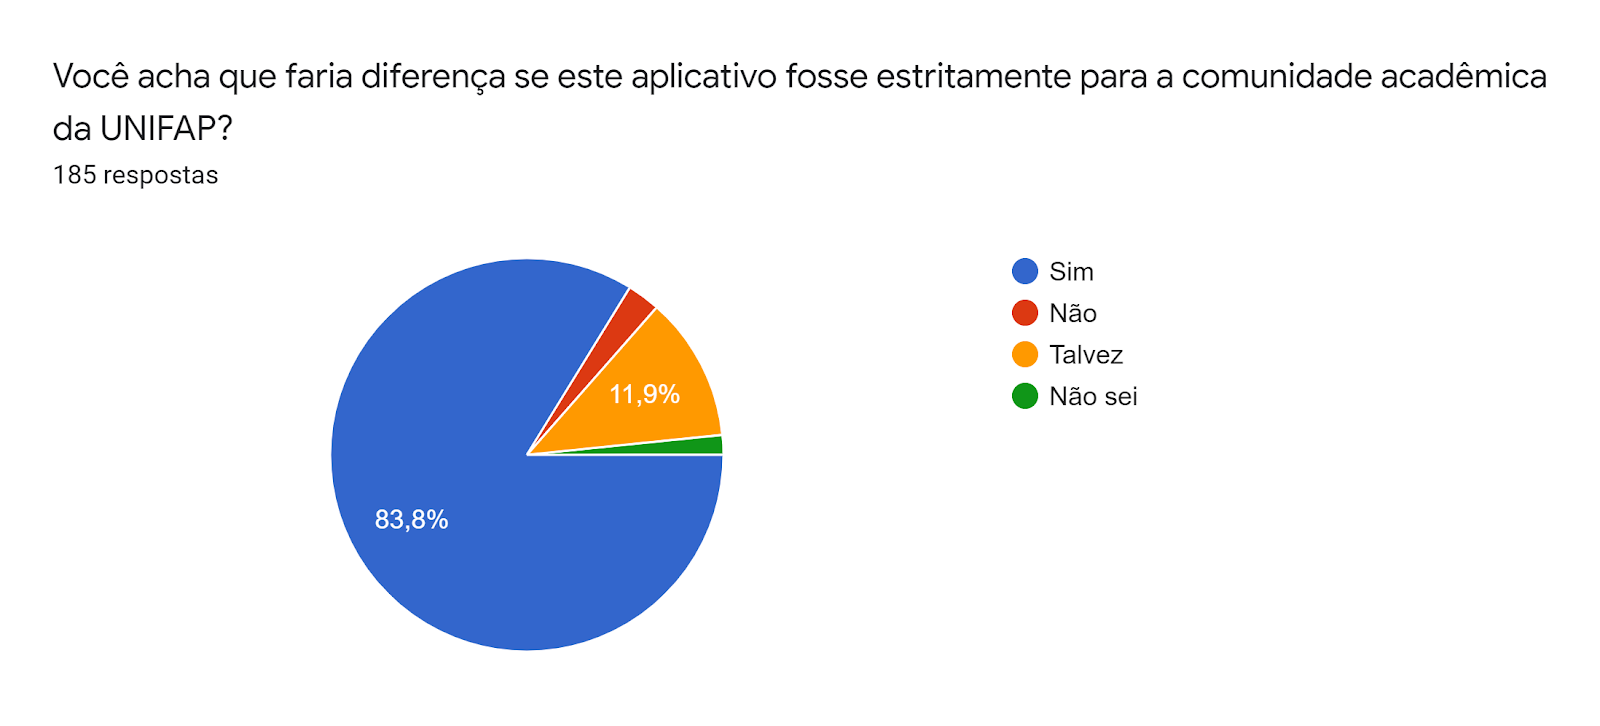
\includegraphics[width=12cm]{./04-figuras/questionario/18.png}
	\label{percepcao}
	\fonte{Elaborado pelo autor}
\end{figure}

\end{comment} %até aqui vai para a seção "resultados preliminares"


%Assim, será definido a metodologia em 3 passos:

% comentado para não aparecer no compilado
	%\mnote{Patrícia: a partir daqui vais falar do terceiro "passo". Ajusta o texto.}
    %
%No terceiro passo realizei o levantamento de requisitos para apresentar um protótipo funcional, desde requisitos funcionais, como o criação de caronas que será restrito apenas para pessoas vinculadas à instituição.

%\textbf{Aqui vai o texto para falar dos passos do caronaê, da apresentação das telas do caronaê}% 

%No terceiro passo detalharei as telas e funcionalidades do aplicativo Caronaê, apresentarei os serviços pensados e utilizados na proposta tanto do projeto Caronaê e quais deles foram reutilizados para a proposta na Unifap.



\begin{comment} % está parte era da proposta de criação do app ou do mockup

\textbf{Foi escrito quando a ideia era criar um app ou um mockup bem traabalhado}
O segundo passo será a construção do UX (User Experience) e UI (User Interface) no software Adobe XD para colocar em prática as primeiras ideias de design do aplicativo, a interface, cores, logo, funcionalidades, entre outros. E para concluir, o quarto passo é os testes, onde será avaliado se as funcionalidades iniciais, junto a isso, estarei finalizando a escrita do documento de trabalho de conclusão de curso.

\textbf{NOTA: MA COISA INTERESSANTE QUE A LORENA FEZ FOI SEPARAR A METODOLOGIA EM "ETAPAS CONCLUÍDAS" E "ETAPAS PENDENTES". VOU CRIAR AS SEÇÕES ABAIXO COMO ELA CRIOU E VC ORGANIZA DIREITINHO.}

\begin{itemize}
\item Questionário
\item Analise dos dados coletados no questionário 
%(parcialmente)
\item Levantamento histórico sobre mobilidade, mobilidade inteligente, campus e cidades inteligentes %(parcialmente, dissertar mais a frente do texto sobre)
\item Levantamento das soluções de mobilidade inteligente
\item Triagem das soluções inteligentes encontradas
\item Primeiros testes com os serviços fornecidos pelo projeto Caronae
\item Teste com o serviço backend do Caroonaê
\item Teste com o aplicativo Android do Caronaê
\item Adequação para testes no código Java do aplicativo Caronaê
\item Levantamento dos requisitos iniciais do aplicativo Caronaê
\item Inclusão das Zonas e bairros da cidade de Macapá no backend do serviço Caronaê
\item Mudança do texto dos campos que estavam UFRJ para UNIFAP
\end{itemize}

\section{Etapas pendentes}

\begin{itemize}
\item Adicionar todos os requisitos da solução esolhida
\item Escrita do trabalho de conclusão final
\end{itemize}

\end{comment}

   	%
% Documento: Referencial Teórico
%

\chapter{Mobilidade Urbana em Cidades Inteligentes}\label{chap:Mobilidade Urbana em Cidades Inteligentes} %referencial teórico  

\begin{comment}
\mnote{Patrícia: Esse capítulo ainda tá um pouco confuso. As seções e subseções tem que conversar. Ainda parece um monte de coisa costurada. A ideia é começar a falar de Cidades Inteligentes e quando falar disso pega o que falamos naquela artigo, sobre a infraestrutura necessária e aí sim vc pode falar de computação e nuvem e PaaS, IaaS e SaaS. 
Na continuação sobre cidades inteligentes vc vai falar mais detalhadamente sobre mobilidade inteligente que é uma das dimensões que aquele autor propõe. Da uma olhada naquele artigo que a ideia eh aquela.
Quando vc falar de mobilidade vc insere o conceito de MaaS e somente depois de tudo isso vc falar sobre campus inteligente. 

Acho que nao cabe aqui ainda falar sobre carona solidária pq seu projeto mudou um pouco o foco devido todos os problemas. Vc vai falar de carona solidária somente na outra seção, quando for apresentar as soluções de mobilidade que foram encontradas, fará o comparativo e chegará na carona solidária.}

\end{comment}

\section{Computação em Nuvem}
A Computação em Nuvem (\textit{Cloud Computing}) vem causando muitas transformações digitais e já tem um lugar de destaque nas CI. Embora atualmente seja algo bastante usual, esse é um assunto grande e complexo que possui vários subtemas, como os modelos de nuvem.

Dentro da Computação em nuvem é comum encontrarmos três modelos de disponibilização de serviços: 

Infraestrutura como serviço, oferece acesso baseado na web para armazenamento e poder de computação. O consumidor não precisa gerenciar ou controlar a subjacente infraestrutura em nuvem, mas tem controle sobre os sistemas operacionais, armazenamento, e aplicativos implantados.

Plataforma como serviço, onde os usuários hospedam um
ambiente para suas aplicações. Os usuários controlam os aplicativos, mas não controlam o sistema operacional, hardware ou infraestrutura de rede que são usados.

Software como serviço, é onde o consumidor usa um aplicativo, mas não controla o funcionamento do sistema, hardware ou infraestrutura de rede. Nesta situação, o usuário orienta os aplicativos pela rede. 

\citeonline{infra-cloud} diz que os serviços oferecidos pela Computação em Nuvem são semelhantes ao serviço de energia elétrica, pagamos apenas o que consumimos. Por consequência, necessidades como as de investir em equipamentos e infraestruturas de TIC são reduzidos.
% permitindo que seus usuários se conectem globalmente sem precisar implementar infraestruturas locais.

%consideravelmente, permitindo que seus usuários se conectem e façam colaborações globalmente sem configurar
%infraestruturas, como servidores, e com uma alta escalabilidade e capacidade de acomodar inúmeros usuários. 

%que seus usuários se conectem globalmente sem precisarem configurar infraestruturas de TI locais.

Vale ressaltar que a capacidade de uma CI ser dinâmica e automática faz ela precisar de infraestruturas robustas e capazes de suprir as necessidades de estar todo tempo online, algo que a computação em nuvem consegue oferecer através de serviços altamente disponíveis, elásticos, flexíveis e robustos. \cite{kon-cloud}.



%A imagem abaixo descreve bem as responsabilidades de cada camada da cloud:

\begin{comment}

\begin{figure}[!hbtp]
\centering
\caption{Camadas de Nuvem e suas responsabiidades.}
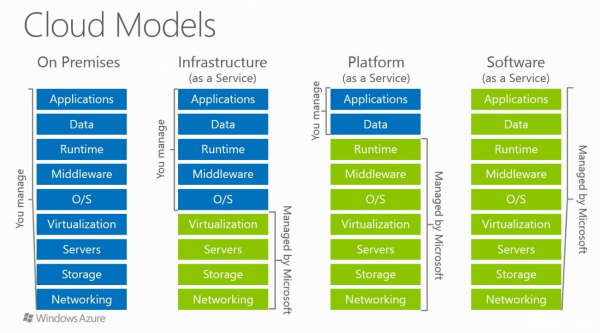
\includegraphics[width=8cm]{./04-figuras/azure-cloud.png}
\label{cloud-computing}
\fonte{https://www.lambda3.com.br/2017/08/iaas-paas-e-saas-qual-a-diferenca/}
\end{figure}
	conteúdo...
\end{comment}



\section{Cidades Inteligentes}

Cidades Digitais, CI, são cidades que utilizam um ambiente inovador caracterizado pela utilização de TIC. Segundo \citeonline{yin} os termos se referem a ação de utilizar a tecnologia em favor da melhoria da qualidade de vida, do gerenciamento de recursos e da infraestrutura das cidades.

Estas cidades sempre buscam otimizar recursos para melhor atender as necessidades dos cidadãos, interconectando informações, gerenciando operações sempre envolvendo uma infraestrutura tecnológica, sistemas inovadores e colaboração digital. \cite{washburn2010helping}.

% isso vale para mobilidade, para o setor imobiliário, saúde e entre outros serviços que de alguma forma podem ser otimizados usando TIC’s \cite{washburn2010helping}.

Já \citeonline{giffinger} acrescentam características para serem considerados antes de desenvolver uma CI. Para os autores, deve ser avaliado um todo, como consciência, flexibilidade, transformabilidade, individualidade, e comportamento estratégico da cidade e de seus cidadãos, e destaca que todos precisam ter conhecimento da posição da cidade e o que precisa ser feito para alcançar o status de CI. 

Segundo \citeonline{neirotti}, TIC não definem uma CI, são apenas uma das soluções utilizadas. O autor ainda explica que as cidades mais equipadas não implicam necessariamente nas melhores CI e o número de iniciativas não indicam performance, apenas demonstra o número de esforços para melhorar a vida dos cidadãos. 


\begin{comment}

De acordo com \citeonline{dameri}: 
\begin{citacao}
“Uma Cidade Inteligente é uma área geográfica bem definida, na qual altas tecnologias, como TIC, logística, produção de energia, etc., cooperam para criar benefícios para os cidadãos em termos de bem-estar, inclusão e participação, qualidade ambiental, desenvolvimento inteligente; é governado por um conjunto bem definido de assuntos, capaz de declarar as regras e políticas para o governo e o desenvolvimento da cidade”. (tradução nossa)."
%\footnote{Texto original: "A smart city is a well-defined geographical area, in which high technologies such as ICT, logistic, energy production, and so on, cooperate to create benefits for citizens in terms of well-being, inclusion and participation, environmental quality, intelligent development ; it is governed by a well-defined pool of subjects, able to state the rules and policy for the city government and development."}
\end{citacao}
\end{comment} 

CI em estudos de \citeonline{giffinger}, citado  por \citeonline{kon}, apresenta uma forma de como as cidades ditas inteligentes podem ser mensuradas e avaliadas, o mesmo cita 6 dimensões que possuem suas características próprias. Na Tabela \ref{tab:tabela1} veremos quais são:

% Please add the following required packages to your document preamble:
% \usepackage[table,xcdraw]{xcolor}
% If you use beamer only pass "xcolor=table" option, i.e. \documentclass[xcolor=table]{beamer}

\begin{table}[h]
\centering
\caption{Aspectos de Cidades Inteligentes}
\label{tab:tabela1}
\vspace{0.0cm}
\begin{tabular}{cp{10cm}}
\hline
 & Definição \\
\hline
\vspace{0.05cm}
Economia Inteligente & 
É a competitividade econômica, empreendedorismo, produtividade, leis que ajudem a inovar e incentivar a criação de novas soluções tecnológicas. \\
\hline
\vspace{0.05cm}
População Inteligente & 
Mede a qualidade da educação da população, seus postos de trabalho e renda, além de avaliar a interação social, os incentivos a programas de educação e incentivos a produção científica e tecnológica. \\
\hline
\vspace{0.05cm}
Governança Inteligente & Avalia o quão transparente e participativo é o governo por meio de seus portais, como são feitas as tomadas de decisões e serviços públicos e sociais.\\
\hline
\vspace{0.05cm}
Mobilidade Inteligente & Trata-se das questões de acessibilidade e mobilidade local onde se leva em consideração os congestionamentos, os transportes utilizados, o uso de combustível fóssil e as soluções tecnológicas que são utilizadas para melhorar o transporte da população.
% sempre priorizando os que menos prejudicam o meio ambiente e o fluxo urbano das cidades.
 \\
\hline
\vspace{0.05cm}
Ambiente Inteligente &
É avaliado quais soluções as cidades possuem para degradar menos o meio ambiente e quais recursos são reaproveitados, como água, energia, lixo.
% energia renovável, lixo reciclado e etc. 
\\
\hline
Vida Inteligente &
A qualidade de vida voltada para a segurança da cidade, da saúde das pessoas, o lazer, qualidade na moradia, serviços culturais.
%Este projeto tem como foco trabalhar apenas na mobilidade inteligente, que por meio de soluções tecnológicas tem melhorado bastante o fluxo nas ruas e estradas brasileiras.

\end{tabular}
\end{table}


\begin{comment}
	Contudo, CI não tem uma definição formal amplamente aceita, embora haja muitos conceitos sobre o tema, Cidade Digital é o que mais se destaca. Alguns autores abordam a diferença entre cidades inteligentes e cidades digitais.
	
	%%Sintetizar este paragrafo, muito grande
	%Segundo  \citeonline{yin}, 
	Cidades digitais se refere a digitalização de uma cidade, envolvendo informações, acesso ao dados e visualizações por parte da população, a cidade digital está mais ligada na forma em que a cidade utiliza e se moderniza com a combinação de comunicação e infraestrutura computacional para fornecer as informações públicas, já cidades inteligentes é uma definição que pode ser considerada como a junção do entendimento de cidade digital e sociedade do conhecimento, onde as pessoas envolvidas são responsáveis pelo aprimoramento do local criando zonas de colaboração digital \cite{yin}.
	%“o objetivo de uma cidade inteligente é transformar a vida e o trabalho dentro de uma região de maneira significativa e fundamental, não incremental” \cite{yin} (tradução nossa).
\end{comment}


Quando se fala a respeito do gerenciamento dos projetos de CI, \citeonline{chourabi} indicam que uma característica comum das iniciativas são que a maioria das cidades inteligentes são gerenciadas e organizadas por governos e utilizam o uso massivo de TIC. 

Uma iniciativa realizada no Brasil, até mencionada por \citeonline{namepardo}, é a da cidade de Porto Alegre, reconhecida nacionalmente e internacionalmente, a cidade tem tomado medidas usando tecnologia para o auxílio desde 2006 quando decidiu investir pesado na implementação de uma rede de fibra ótica para os serviços do governo , garantindo mais de 99.8 \% de disponibilidade \cite{weiss}.

 São Paulo se destaca também como o maior centro de pesquisa sobre o tema com muitas publicações e diversos trabalhos relacionados às áreas envolvidas, tendo a USP entre os destaques no número de publicações \cite{lazzaretti}. 


E para alcançarmos um nível de CI, algumas coisas precisam ser pensadas antes. Soluções que auxiliem questões como segurança, saúde, educação, ou mesmo lazer são fundamentais. Ações desde a construção de áreas verdes, de centros de cultura e monitoramento da cidade utilizando câmeras e mapeamento de zonas pouco seguras são essenciais. 

No entanto, a população não irá usufruir de nenhuma das soluções desenvolvidas para quaisquer das dimensões apontadas se não acontecer uma inclusão tecnológica massiva com programas de incentivo à educação científica e tecnológica. Caso contrário, parte da população será excluída e segregada da cidade \cite{patricia}.

Além disso, para construir uma CI fatores importantes como inclusão digital e infraestrutura tecnológica precisam ser discutidos. Para que estás soluções funcionem de maneira efetiva é necessário que elas sejam desenvolvidas considerando um sistema de computação que tenha uma arquitetura heterogênea e distribuída. As arquiteturas mais utilizadas atualmente são as em nuvem, devido sua capacidade de suportar grande demanda e a escalabilidade \cite{patricia}. 

\begin{comment}
	A arquitetura se dá primeiramente através de dispositivos de borda que são responsáveis por coletar dados dos dispositivos de internet da coisas espalhados pelo ambiente, a característica desses dispositivos é de serem de baixo processamento e capacidade. Após o processo de coleta, os dispositivos de borda enviam os dados para a nuvem para serem processados e armazenados. A rede tem características homogêneas com extrema importância de serem altamente disponíveis e capazes de oferecer acesso de milhares de pessoas por meio de seus dispositivos. Mais uma vantagem da computação em nuvem é se tratando de valores, segundo \cite{patricia}, a contratação de serviços em nuvem diminui os altos gastos em infraestrutura, a contratação conforme as necessidades das aplicações trazem uma grande vantagem, economia que não cria problema para os usuários, os serviços de nuvem oferecidos devolvem o resultado esperado.
\end{comment}


\section{Mobilidade Inteligente}
%\mnote{compartilhamento de carros}
%\mnote{compartilhamento de viagens}
%\mnote{transporte sob demanda}
%\mnote{Falar sobre as tecnologias que tornam possível a utilização de ferramentas de mobilidade inteligente; gps, smartphones, cloud}
%Com o passar dos anos, A mobilidade urbana está necessitando cada vez mais de atenção. 

%Com o aumento do número de pessoas e veículos surgem alguns problemas  como engarrafamentos cada vez maiores, dificuldade de locomoção de pedestres e ciclistas, poluição do ar. 

%No entanto, \citeonline{santana} diz que a Mobilidade Urbana vai além de trânsito lento e grandes congestionamentos, a mobilidade urbana carrega a importância da cidadania de um povo.

\citeonline{giffinger} afirma que mobilidade inteligente trata-se de acessibilidade nacional e internacional dando importância as tecnologias modernas advindas da TICs e sistemas de transporte sustentáveis. O uso de uma tecnologia moderna que de suporte a mobilidade faz surgir sistemas "inteligentes".

Além disso, otimizar a logística dentro de áreas urbanas, fornecer aos cidadãos um sistema dinâmico e multimodal, assegurar um transporte sustentável e ecológico e ainda levar em consideração as condições de tráfego e energia melhoram o transito urbano e mobilidade dos habitantes \cite{neirotti}. %\cite{giffinger}.

Modais como ônibus, metros, carros e bicicletas são avaliados em relação a sua facilidade de mobilidade. Analisar o tamanho da malha viária, ciclovias, uso de transporte poluentes e não poluentes, uso de transporte público também são parâmetros considerados \cite{kon}. 

Muitas iniciativas começaram a criar soluções tecnológicas com objetivos de tratar essas "dores" \cite{cocchia}. Dois projetos na cidade de Mdadrid (Espanha) que utilizam os celulares dos cidadãos, um de monitoramento em tempo real da posição do transporte publico e outro informando estimando a lotação dos coletivos são dignos de nota.

Hoje em dia é possível monitorar todo e qualquer tipo de transporte, o GPS é um dos dispositivos que nos auxiliam nisso. Na cidade de São Paulo, a Startup Scipopulis monitora em tempo real 14 mil ônibus obtendo dados da velocidade média das vias, acidentes ocorridos naquele momento, a quantidade de ônibus transitando na mesma via. Todos essas informações são passadas para a companhia da transporte da cidade para possíveis melhorias na mobilidade da cidade de São Paulo \cite{kon}.


%Diante do exposto, a Mobilidade Urbana

%Das várias iniciativas de cidades inteligentes, a mobilidade tem um lugar de destaque por apresentar várias soluções que já apresentam uma melhora no trajeto das pessoas em várias cidades utilizando TIC. 



% a exemplo disso, aplicativos como Uber, 99 circulam pelas cidades utilizando a mobilidade como um serviço.

%Aplicativos de carona como o BlaBlaCar  que a relação entre o motorista e o passageiro fica a critério do motorista em relação aos custos da viagem. Estas ferramentas já contribuem com a melhoria da mobilidade sem a necessidade de investimento público. 

%Uma mudança que estas aplicações apresentam é a de lugares ocupados dentro de um mesmo veículo. Segundo pesquisa realizada pela BlablaCar em 2018, a taxa de ocupação de pessoas usando o aplicativo por veículo no Brasil é de 3,8 incluindo o motorista, contra 1,9 pessoas por veículo sem o uso de do aplicativo, na mesma pesquisa, a empresa apresenta dados que as caronas solidárias ajudam na economia de CO² alegando que pessoas que  fazem o mesmo trajeto todo dia e possuem carros podem participar de um rodízio de caronas, por exemplo, nesta conta, teríamos todo dia 1 carro a menos nas ruas.

%Hoje em dia são algumas dessas soluções, aplicativos como BlaBlaCar, outros aplicativos de carona solidária mobilizado por universidades como o Caronaê da UFRJ\footnote{Disponível em: https://caronae.org/. Acesso em: 23 Jun. 2020.}, entre outras,  que movimentam o conceito de mobilidade urbana inteligente no país.

%1 - O que é?

%2 - A mobildade urbana e inteligente

%3 - A importancia da mobilidade inteligente

% serviços já existentes (uber, 99, falar um pouco de maas); mobilidade como serviço
% carona solidária

%Cocchia (2014) -a adoção de políticas de crescimento requer que as cidades
%passem a buscar projetos com o fornecimento de soluções para mobilidade urbana. As cidades
%inteligentes incialmente eram chamadas de cidades digitais por incorporar ao seu conceito
%apenas o uso de tecnologia da informação. Com a evolução passaram a incluir os conceitos de
%sustentabilidade aos seus projetos. A mobilidade urbana em cidades inteligentes faz surgir o
%5conceito da “mobilidade urbana inteligente”.

\section{Campus Inteligente}

Um campus inteligente é o reflexo de uma cidade em uma escala menor, nos campos temos relações sociais, relações administrativas, meio ambiente, serviços de coleta, mobilidade, alimentação, energia, entre outros.

Conforme \citeonline{zhang}, o comportamento de uma Campus Universitário Inteligente é semelhante ao de uma CI, porém, com um número de problemas menores, e de proporções menores, onde pode ocorrer roubos, acidentes de carro, circulação de pessoas em lugares proibidos ou outras situações não permitidas \cite{garay2018}.

Assim como cidades inteligentes, campus inteligente ou universidade inteligente não tem um conceito totalmente definido, \citeonline{alghamdi} explica que o campus inteligente surge da necessidade de oferecer serviços de alta qualidade reduzindo custos, e que isso não fica apenas nos aspectos acadêmicos, mas envolve aspectos sociais, meio ambiente, e financeiros da Universidade.

\begin{comment}
Na Figura \ref{alghamdi}, temos:
\begin{figure}[!hbtp]
\centering
\caption{Conceito de Campus Inteligente, seu impactos e suas aplicações.}
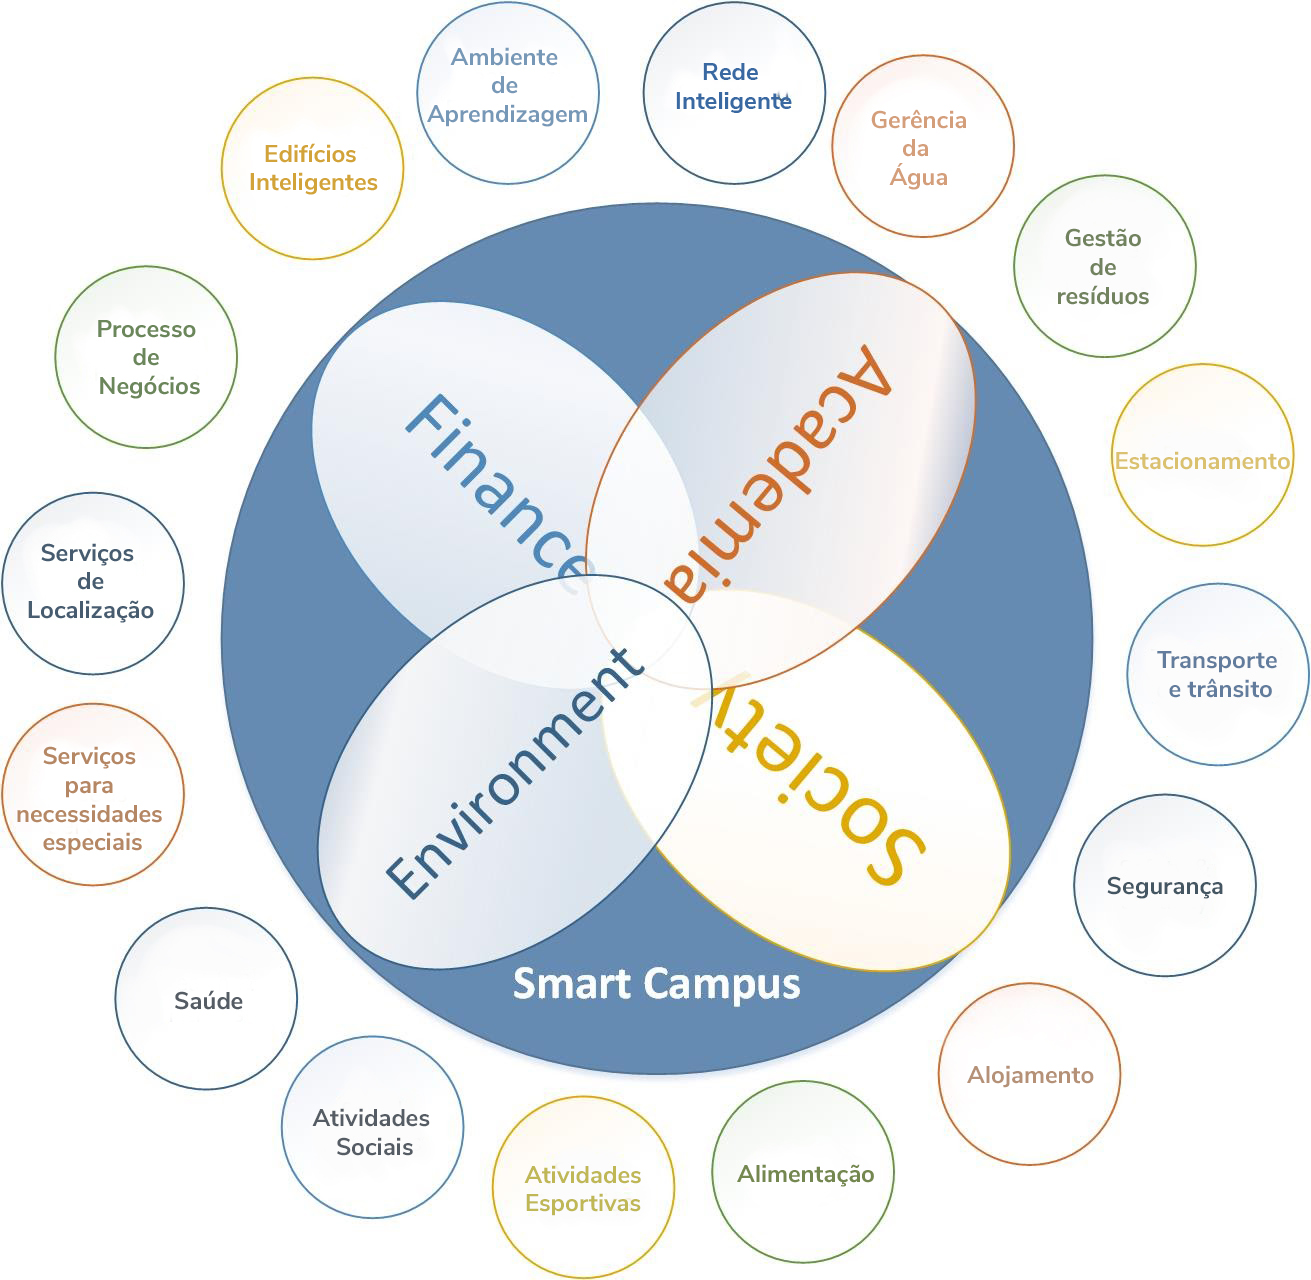
\includegraphics[width=8cm]{./04-figuras/alghamdi-edited.jpg}
\label{alghamdi}
\fonte{Adaptado de \citeonline{alghamdi}}
\end{figure}
\end{comment}




Além do conceitos e objetivos, o Campus Inteligente também tem problemas e dificuldades que o mercado impõe. \cite{alghamdi} cita 3 obstáculos: Técnico, Financeiro e Político. Semelhante as Cidades Inteligentes, deve-se considerar que ao estabelecer serviços tecnológicos a uma população, que seja de uma cidade, ou de uma universidade, conceitos de segurança, proteção e privacidade, interoperabilidade, padronização e configurações precisam estar bem encaixados para promover segurança ao uso por pessoas do Campus/Cidade, e reunir esses requisitos num ambiente tão heterogêneo, de comunicação intensiva é uma tarefa difícil \cite{alghamdi}. 

Do lado financeiro, conseguir dinheiro para levar adiante projetos que necessitam de investimentos algumas vezes elevados e experiências imaturas, ou até mesmo, sem experiência alguma com Campus Inteligente acaba dificultando iniciativas ao redor do mundo . Finalmente, os obstáculos políticos em um ambiente universitário
não são tão difíceis quanto as técnicas e financeiras devido ao
fato de que o presidente de uma universidade pode resolver a tomada de decisão processo em muitos casos; no entanto, a colaboração entre
diferentes faculdades e departamentos, reengenharia de negócios
processos e oposição de funcionários anti-tecnologia são potenciais
obstáculos que precisam ser resolvidos \cite{alghamdi}.

Por outro lado, as iniciativas tecnológicas abrem portas para recrutarmos pesquisadores, investigarmos mais sobre o tema e promover serviços e soluções inovadoras, segundo \cite{alghamdi}, a maioria dos trabalhos focados em Campus Inteligentes são sobre energia, meio ambiente e prédios inteligentes, e alguns serviços importantes, como transporte, alimentação, controle de tráfego ficam deixadas de lado.

\section{Mobilidade com Serviço - MaaS}

Mobilidade como um serviço (Mobility as a Service) é um termo utilizado para nomear uma nova tendência na mobilidade inteligente, onde empresas, organizações investem no transporte público oferecendo meios multimodais de locomoção  para a população. Algumas das características de plataformas MaaS é a facilidade de acesso, a ferramenta apresenta as opções que o usuário pode escolher para seu trajeto, facilidade no pagamento, sistema de reserva de viagens e informação em tempo real.

Sem uma definição exata, o MaaS é definido por alguns autores como a oferta de serviços de mobilidade centralizados em uma única plataforma digital, focando exclusivamente nas necessidades individuais dos usuários, sendo estes, táxis, transporte público coletivo, carros particulares, bicicletas, entre outros \cite{jittrapirom, kamargianni, mulley}.

Para não aprofundar, o objetivo da MaaS é incentivar o uso de transportes compartilhados e que seja possível o usuário planejar o seu trajeto em cima de várias opções multimodais, sejam elas, compartilhamento de carros, caronas, compartilhamentos de bicicletas, aluguel de carros, transporte público, entre outros meios de mobilidade \cite{jittrapirom}. 

\begin{comment}




\subsection{Carona Solidária}

No dicionário online define-se Carona como uma viagem sem custos para o passageiro, onde a pessoa vai pro mesmo ou para um destino próximo do destino do motorista \cite{carona}.

Carona solidária ou Carpooling consistem em compartilhar um veículo entre vários passageiros durante um trajeto para ir ao trabalho, ir a escola, a universidade, ou qualquer outro trajeto em que o ponto final seja definido. O carpooling tem ganhado mais notoriedade quando se torna um amigável e mais barato meio de transporte \cite{aissaoui}.

A carona solidária é uma prática que vem sendo utilizado por várias empresas, sejam públicas ou privadas com o objetivo de aproximar seus empregados, estreitar laços criando relações de confiança, compartilhar conhecimento e tornar os profissionais mais colaborativos \cite{oliveira2013educaccao, arasaki}. A carona solidária tende a criar relações de maneira mais amigável, assim, as pessoas tendem a conversar mais, compartilham experiências, problemas \cite{oliveira2013educaccao}.

Ainda sobre caronas solidárias, as iniciativas de carona solidária estão sendo implementadas por muitas universidades com a intenção de melhorar o acesso à instituição, sendo abordada sempre com a utilização de aplicativos e como uma medida de mobilidade inteligente e mobilidade colaborativa \cite{figueira2015mobilidade}.

Além disso,  a prática da carona solidária é vista como uma medida que impulsiona o desenvolvimento da mobilidade sustentável, onde carros antes ocupados por apenas uma pessoa será ocupado por outras, podendo haver um revezamento de carona entre os motoristas que realizam o mesmo trajeto todos os dias, sendo assim, vamos ter menos carros, logo menos poluição \cite{silveira,carpooling2013, arasaki}.



\section{Consumo Colaborativo}

Consumo colaborativo, economia colaborativa ou economia compartilhada são termos que se referem ao uso compartilhado de bens e produtos entre proprietário e cliente, o consumo colaborativo não exigem que o cliente adquira o produto, apenas “alugue”, neste novo modelo de consumo, o proprietário pode “vender” o produto por diversas vezes.

Com esse novo modelo, muitos serviços que antes funcionavam de uma forma estão mudando, a exemplo, consumo de carros, apartamentos, equipamentos, tempos e habilidades \cite{bardhi2012access}. Ebay\footnote{Disponível em: https://www.ebay.com/. Acesso em: 11 de Jul. de 2020.} (comércio eletrônico), ZipCar\footnote{Disponível em: https://www.zipcar.com/. Acesso em: 11 de Jul. de 2020.} (aluguel de carros), Freecycle\footnote{Disponível em: https://www.freecycle.com.br/. Acesso em: 11 de Jul. de 2020.} (rede de trocas de bens e serviços), iniciativas de Crowndfounding\footnote{Disponível em: https://conceitos.com/crowdfunding/. Acesso em: 13 de Jul. de 2020.} e espaços de Cowork, são ferramentas voltadas para o consumo colaborativo, cada uma em seu mercado específico \cite{santospereira}.

Diante disso, \cite{mendes2015economia} explica que a economia compartilhada vem mudando a principal característica do capitalismo mundial, onde a aquisição de bens por parte do comprador é dispensável, existindo apenas uma troca, uma facilidade de acesso ao produto sem necessidade de posse, uma relação de necessidade e posses.

Segundo \cite{bostman2011s}, o consumo colaborativo reflete sobre 3 tipos diferentes: 

\subsection{Sistema de Serviços de Produto (SSP)}

Permite compartilhar vários produtos de uma empresa (carros, filmes, objetos, acessórios), um melhor exemplo de um SSP são os casos de Netflix, Spotify, ambos oferecem os seus serviços e gerenciam direitos digitais. No Brasil várias startups trabalham nesse tipo de consumo, compartilhando bicicletas, patinetes, carros, bolsas \cite{santospereira}.


\subsection{Mercado de Redistribuição}

O mercado de redistribuição está ligado a forma de como lidamos com coisas que não nos servem mais, o passando adiante sem desperdiçá-lo, jogá-lo fora, em vez disso, mudando ele de um lugar que não é útil para um lugar que terá utilidade, esse tipo de consumo colaborativo é baseado nos princípios “reduza, reuse, recicle, recupere e redistribua” (APRENDA INVESTIMENTOS, 2016). 

\subsection{Vida Colaborativa}

Como \cite{bostman2011s} definem que a vida colaborativa é o estilo de vida onde pessoas compartilham coisas intangíveis, como seu tempo, espaço e habilidades, espaços de coworking ou pessoas que buscam outras pessoas para compartilhar conhecimento através de ferramentas também são exemplos disso.

\end{comment}
   	%\chapter{Fundamentação Teórica}
\chapter{Ferramentas}
\section{Java}

Java é uma linguagem de programação orientada a objetos criada em 1990 pela empresa Sun Microsystems e hoje pertence a Oracle. O java é uma lingaguem multiplataforma, podendo ser utilizando tanto em navegadores quanto em dispositivos para smartphones, Windows, linux e outros perífericos isso porque o código Java não é compilado para uma linguagem de máquina e sim para uma linguagem intermediária chamada bytecode que é interpretada e executava pela máquina virtual (JVM) Java.

\section{Android Studio}

O Android Studio é chamado de Ambiente de Desenvolvimento Integrado (ou IDE, sigla em inglês para Integrated Development Environment), um programa de computador que reúne as características e ferramentas de apoio para a criação de aplicativos para dispositivos móveis para Android. Hoje suportando duas linguagens de programação, Java e mais recente, Kotlin, as duas voltadas para o desenvolvimento de aplicações Android.

\section{Laravel}
Gratuito, de código aberto, com suporte a recursos avançados e facilidade na construção do código, simples e legível com a utilização do padrão MVC: essas são as principais vantagens do Laravel, o que torna ele o framework preferido por muitos desenvolvedores. O Laravel se tornou o framework mais utilizado por desenvolvedores PHP que trabalham nessa ferramenta utilizando o padrão de desenvolvimento.%https://www.tecmundo.com.br/software/223718-laravel-conheca-o-framework-php-utilizado.htm

\section{MVC}

É um padrão de projeto de software que significa Model, View e Controller, fácil e eficiente, este padrão tem como pontos positivos trabalhar com reuso de código e dividir em 3 camadas a estrutura do projeto, o deixando a solução fácil e eficiente

\textbf{Model:} É a camada responsável pela regra de negócio da aplicação, é onde está as informações necessárias que toda a solução irá precisar para funcionar, desde consultas ao banco de dados, validações, notificações, entre outras coisas que serão consultadas em algum momento na aplicação.

\textbf{View:} Será onde todas essas informações e ações serão exibidas para o usuário, é na View que as informações são renderizadas, a parte interação homem-máquina fica responsável por essa camada.

\textbf{Controller:} O meio de campo das duas aplicações, o Controller fica a parte do código que gerencia o momento de chamar cada função, cada ação que deverá ser executa. O controller recebe instruções dá View, encaminha para o Model e as retorna quando necessário.

\section{Firebase}

Firebase é uma plataforma digital desenvolvida pela google utilizada para facilitar o desenvolvimento de aplicativos web ou móveis, de uma forma efetiva, rápida e simples. Suas funcionalidades principais são Firebase Authentication, que fica responsável por toda da parte de autenticação dos aplicativos, Cloud Messaging, responsável por toda parte de notificações da aplicação, podendo notificar várias plataformas, e o Realtime Messaging, onde é utilizado para mensagens instantâneas, a exemplo, o Whatsapp.

\section{PostGresSQL}

É um banco de dados objeto relacional de código aberto muito utilizando em todo o mundo, por ser seguro, robusto, de alto desempenho e multitarefa, o PostGresSQL é recomendado para projetos que precisam de alta disponibilidade, persistência num grande volume de dados, além de ter uma ferramenta de fácil aprendizado.



\section{Heroku}

O Heroku é uma plataforma como serviços (PaaS) utilizada para facilitar o deploy de aplicações backend, testes em produção ou hospedagem de sites ou APIs. Bastante utilizada, o Heroku tem integrações com o GitHub, facilitando ainda mais a vida de seus usuários, suas atualizações de código são automaticamente replicadas para a aplicação na medida que o seu repositório é alterado no GitHub.
   	%
% Documento: Soluções Existentes
%


						
\chapter{Soluções de Mobilidade Inteligente Existentes}\label{chap:Soluções Existentes} 
%

%Carros híbridos, carros elétricos, patinetes elétricos, compartilhamento de carros. chips, gps,smartcards, protocolo its são responsável por isso ser possível

%\textbf{Como FUNCIONA, PERGUNTA A SER FEITA PARA CADA SOLUÇÃO DE MOBILIDADE INTELIGENTE}

A mobilidade urbana e o transporte são vitais para o funcionamento das cidades inteligentes. Mobilidade urbana significa acessibilidade local, nacional e internacional da CI, disponibilidade de infraestrutura de TIC, bem como sistema de transporte inovador e seguro.  O atual surgimento de soluções sistêmicas nos transportes é uma parte do movimento em direção à mobilidade sustentável. Permite não só o bom desenvolvimento de uma cidade, mas também ajuda a superar dificuldades notadamente visíveis em áreas urbanizadas e densamente inibidas, como engarrafamentos, emissões poluentes, congestionamento sonoro, separação de espaços habitacionais e outros \cite{opitek}.

Para \citeonline{dameri}, o envolvimento das TICs proporcionou inúmeras iniciativas para cidades inteligentes, como por exemplo monitorar a mobilidade urbana inteligente e outras tecnologias como redes inteligentes, veículos de combustível alternativo e assim por diante, o autor ainda afirma que cada tecnologia incentiva várias outras iniciativas e projetos que podem melhorar a qualidade de vida, a redução da poluição, a redução dos congestionamentos, entre outros.

A exemplo dessas tecnologias, foi através do GPS que muitas iniciativas foram postas em prática. A tecnologia  que disponibiliza a localização em tempo real foi responsável pelo surgimento de mapas digitais -- A ferramenta Google Maps é um exemplo claro disso -- que desencadeou uma série de soluções de mobilidade inteligentes. Soluções que fornecem a localização em tempo real de transportes coletivos, de veículos, pessoas, que possibilita planejar um itinerário, de saber onde outra pessoa se encontra e podendo verificar o melhor trajeto para chegar até ela, são uma das várias soluções existentes e possíveis de encontrar atualmente.

E para isso, vamos exemplificar algumas das categorias dessas opções de mobilidade existentes que nos  dividimos em 4 modalidades:
% Nome dos novos tópicos
\begin{itemize}
	\item Orientações de Mobilidade
	\item Transporte Individual Privado de Passageiros por Aplicativo
	\item Viagens Compartilhadas por Aplicativos
	\item Veículos Compartilhados
\end{itemize}

\section{Orientações de mobilidade}

Essa categoria agrupa plataformas que atuam no auxílio à orientação para os deslocamentos da cidade. Portanto, são usadas indistintamente por motoristas a serviço de outros ou pelos próprios indivíduos em deslocamento. Os exemplos mais conhecidos são o Google Maps e o Waze Mobile, ambos presentes em vários países. Como se baseiam no sinal de GPS, que tem
abrangência mundial, são frequentemente escalonáveis para corresponder a essa abrangência,
dependendo apenas do efetivo mapeamento de ruas. \cite{caronae}

%Dissertação de Luísa (texto sem mudanças)

\subsection{Waze}

A Waze foi fundada em 2008 em Israel, originalmente chamada de LinQmap, e em 2011 já
empregava 80 pessoas. Seu diferencial, se comparada aos sistemas de navegação por GPS tradicionais, vem do fato de se basear em uma comunidade de usuários, aproveitando-se da localização fornecida por cada usuário através de seus Smartphones. 
%para alimentar seu banco de dados.
% Foi a primeira plataforma a funcionar desta forma, antes mesmo da Google lançar essa funcionalidade em seu aplicativo de mapas. As informações enviadas pelos usuários possibilitam a atualização da plataforma em tempo real, gerando informações muito precisas sobre o fluxo de tráfego, por exemplo.

Daí inferimos outra categoria de classificação importante, do ponto de vista da mobilidade
urbana: aplicativos uni ou multimodais. O Waze, desse ponto de vista, por ser uni modal – e o modal em questão ser o carro particular –, pode melhorar as escolhas de trajetos dos motoristas, aliviando o tráfego e diminuindo o tempo de viagem.
% o Google Maps, ao permitir a visualização de diferentes tempos de deslocamento segundo cada modal (de carro, de ônibus, a pé, de bicicleta ou mesmo de avião, quando o trajeto permite), estimula a exploração dos diferentes modais (ainda que a combinação de modais para um mesmo trajeto seja ainda pouco explorada), o que pode acabar levando a escolhas mais sustentáveis, em especial para deslocamentos menores. 

%Dissertação de Luísa (texto sem mudanças)

\subsection{Cittamobi}
O Cittamobi é um aplicativo de transporte público disponível em plataformas iOS e Android com finalidade de fornecer mapeamento, cadastros, monitoramento, previsões e informações de ônibus, linha e rotas calculadas em tempo real. O aplicativo utiliza a localização atual do usuário e o local de destino para encontrar o ponto de ônibus, a linha e o tempo que cada veículo vai demorar até chegar. Na figura \ref{fig:cittamobi} vemos algumas telas do aplicativo Cittamobi.

\begin{figure}[!hbtp]
	\centering
	\caption{Telas do aplicativo de orientações de mobilidade Cittamobi}
	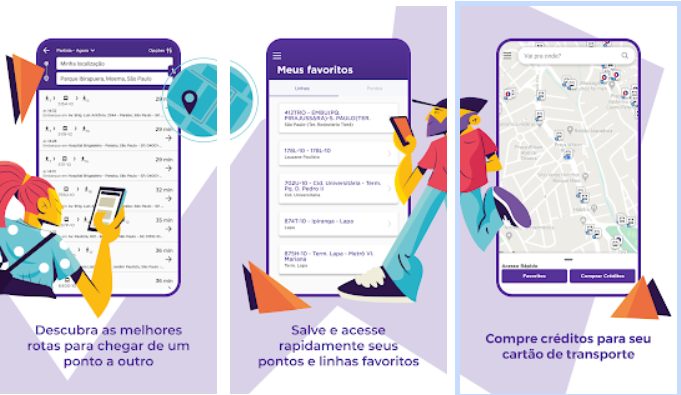
\includegraphics[width=0.4	\textwidth]{./04-figuras/cittamobi/cittamobi.png}
	\label{fig:cittamobi}
	\fonte{Loja de aplicativos do Android: PlayStore}
\end{figure}



%\subsection{Moovit}

\section{Transporte Individual Privado de Passageiros por Aplicativo}

A mobilidade vem mudando durante os anos, surgem novas maneiras e ferramentas para o uso da mobilidade, aplicativos como Uber, Cabify, BlaBlaCar, Yet Go, entraram no mercado e se tornaram ferramentas muito úteis, de grande uso, e ajudando tanto na mobilidade da população quanto no trânsito de muitas cidades, levando em consideração que pessoas que utilizam bastante deixam de ter a necessidade de possuir um carro para utilizar apenas esses serviços, baseado no conceito de consumo compartilhado que vimos anteriormente.

Esse novo conceito, essa nova abordagem de mobilidade é inserida nas cidades não apenas com as ferramentas citadas acima, mas outras iniciativas, como de universidades também tentam melhorar a mobilidade de seus determinados públicos através de aplicativos de carona solidária, pontos de parada de compartilhamento de corridas.

Inspiradas pelo crescente sucesso da Uber, surgiram startups visando de atuar de forma similar, mas voltados para o mercado de motoristas de táxi, algumas delas cresceram e se destacam por sua abrangência cada vez maior, como é o caso da Easy Taxi, empresa brasileira fundada em 2012 no Rio de Janeiro, presente em mais de 30 países e 420 cidades atualmente \cite{caronae}.
%texto não modificado

\subsection{Uber}
A história da Uber teve início quando seus fundadores, Garrett Camp e Travis Kalanick, em Paris, encontraram certa dificuldade para encontrar um táxi. Percebendo a demanda por transporte, os executivos resolveram criar uma plataforma que permitisse solicitar carros premium. A Uber foi fundada em 2009, na Califórnia, como um aplicativo para facilitar o acesso ao transporte.

A Uber chegou ao Brasil em 2014, com atuação no Rio de Janeiro. A segunda cidade a receber o aplicativo foi São Paulo, seguida por Belo Horizonte. Atualmente, mais de 100 cidades brasileiras contam com os serviços da empresa, realizados por 500 mil motoristas parceiros. 

%https://canaltech.com.br/empresa/uber/#:~:text=A%20hist%C3%B3ria%20da%20Uber%20teve,dificuldade%20para%20encontrar%20um%20t%C3%A1xi.&text=A%20Uber%20foi%20fundada%20em,facilitar%20o%20acesso%20ao%20transporte.

\begin{comment}
\subsection{99}
Fundada em 2012, a 99 é fruto da vontade de fazer diferente de três conhecidos geeks da internet brasileira: Ariel Lambrecht, Renato Freitas e Paulo Veras. Seis anos depois, fomos adquiridos pela DiDi, a maior plataforma de transporte por celular do mundo que atinge mais de 60\% da população mundial e cobre mais de mil cidades com um serviço de mobilidade cada dia melhor. Além do nosso trabalho constante pelo melhor serviço, perseguimos a missão de impactar positivamente a população, tornando o transporte mais barato, rápido e seguro para passageiros e o dia a dia mais rentável e tranquilo para motoristas através da tecnologia. E para que isso aconteça, damos poder de escolha para todos com as nossas categorias de serviço, que vão desde o 99Pop, com motoristas particulares em diversas cidades; até o 99Táxi, presente em todo o Brasil no modo tarifa cheia e desconto, que oferece a comodidade do táxi com valores até 30\% mais baixos; e o 99Top, um serviço premium com táxis de luxo. Assim, no brasil, conectamos 14 milhões de passageiros a 300 mil taxistas e motoristas e mudamos a vida de milhões de pessoas todos os dias, reinventando o seu jeito de ir e vir. 
%https://www.revelo.com.br/empresas/99taxis
    
\end{comment}

\subsection{Cabify}

Cabify é um dos grandes nomes no seguimento de aplicativos de viagem e deslocamento. A empresa é conhecida como uma multinacional de rede transporte, concorrente de outros serviços como, por exemplo, Uber e 99.

Em Cabify, a dinâmica é bem parecida com outros aplicativos de carona no mercado, seus usuários podem pedir por corridas para lugares determinados através de sua geolocalização.

No entanto, a plataforma conta com alguns diferenciais oferecendo o serviço de táxis e motoristas profissionais, além disso, é possível programar corridas de acordo com o dia e horário desejados, recurso que ainda foi pouco explorado por outros aplicativos. 

%https://canaltech.com.br/apps/cabify-o-que-e-como-funciona/%

\section{Viagens Compartilhadas por Aplicativos}
\subsection{BlaBlaCar}

 O BlaBlaCar é um aplicativo de caronas bastante utilizado para corridas intermunicipais, o valor fica a critério do caroneiro em negociação com o motorista. O aplicativo surgiu em meados de 2003 devido a necessidade de Fred (Fundador da BlaBlaCar) de ir visitar sua família no interior da França sem carro e com as passagens de trem esgotadas, ele pediu que sua irmã fosse buscá-lo, durante o caminho, ele notou que muitos carros andavam com muitos lugares desocupados, então, ele viu nessa situação um começo de um novo modal (BlaBlaCar, 2020).
        
O aplicativo é diferente dos citados acima por ser aberto para todos, basta realizar o cadastro e já pode compartilhar suas caronas. Comparado a outros aplicativos voltados à remuneração como Uber e 99, o BlaBlaCar costuma ter viagens mais longas, intermunicipais por exemplo, à um preço bem mais acessível. %texto escrito por mim

\subsection{Bynd}

A empresa foi criada no final de 2014 em decorrência de uma experiência pessoal de seus dois sócios-fundadores, Gustavo Bertazzola Graciteli e Leonardo Fernandes Libório, que fizeram uma viagem pelas Américas por 13 meses em um carro compartilhado com outras três pessoas. Após esse período sabático, ambos decidiram abandonar suas carreiras no mercado financeiro e iniciar um novo negócio. A ideia de criar a Bynd surgiu em uma palestra para empreendedores. na qual um dos diretores da Tecnisa (empresa do mercado imobiliário brasileiro) apresentou problemas que careciam de soluções mais eficazes; entre elas, a dificuldade em disponibilizar vagas de estacionamento aos funcionários da empresa. Assim, a Bynd surgiu para melhorar a taxa de ocupação dos veículos, melhorando a eficiência dos deslocamentos realizados por meio de carons corporativas.

% texto da Tesé André

O suporte da tecnologia da informação e comunicação foi imprescindivel para a que a Bynd oferecesse seus serviços, entre eles: a disponibilização do aplicativo para dispositivos móveis e do \textit{website}; a implementação de salas de bate-papo para facilitar a comunicação direta entre os usuários; a realização de atendimentos virtuais; o desenvolvimento dos mecanismos de premiação e de incentivos; as consultas às caronas disponíveis em tempo real; o envio de notificações, entre outros. Embora cientes da possibilidade de extrair dados de dispositivos da Internet das Coisas e de \textit{big data}, esses recursos ainda não foram implementados; contudo, os fundadores ressaltam que a previsibilidade e a confiabilidade são requisitos essenciais para a operação de seu modelo de negócio, e ambos são suportados pelas TIC. 

%texto da tese André

\subsection{Vemcar}

Desenvolvido na Universidade Federal do Rio Grande do Norte, o aplicativo Vemcar começou a ser desenvolvido em uma disciplina oferecida no curso de Engenharia de Software, logo após, o protótipo passou para a equipe da Superintendência de Informática da Universidade Federal do Rio Grande do Norte (SINFO), lá foi realizado toda a validação da ideia, surgimento dos requisitos e foram aplicadas as regras do um processo de software. No Vemcar somentes pessoas ligadas à universidade( professores, alunos, técnicos) podem utilizar o aplicativo.

%texto escrito por mim

\begin{figure}[!hbtp]
	\centering
	\caption{Aplicativo de Carona Solidária Vemcar}
	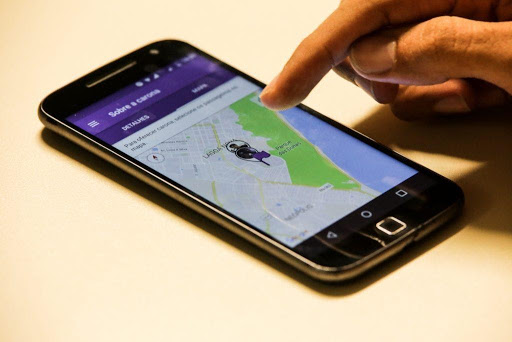
\includegraphics[width=0.5\textwidth]{./04-figuras/vemcar.jpg}
	\label{fig:tecnologia}
	\fonte{https://www.ufrn.br/imprensa/materias-especiais/2872/aplicativo-de-caronas-solidarias-da-ufrn-registra-mil-downloads-em-uma-semana}
\end{figure}


\subsection{Caronaê}

%mencionar trabalho da luísa e do artigo publicado sobre o aplcativo.

O Caronaê é um aplicativo de carona voltada para o ambiente universitário desenvolvido por alunos da Universidade Federal do Rio de Janeiro (UFRJ). O aplicativo está disponível para duas plataformas, Android e iOS. Em seu site oficial (CARONAÊ, 2020) diz que \textit{“O Caronaê é um sistema de código aberto, seguro e prático de caronas compartilhadas, criado com o objetivo de ser replicado em diferentes instituições e feito exclusivamente para a comunidade acadêmica das instituições integrantes da Rede Caronaê”}.

Dos pontos interessantes que o aplicativo oferece são, o uso exclusivo da comunidade acadêmica, a centralização das ofertas de carona, o aumento da taxa de ocupação dos veículos e pontos de carona para facilitar o encontro de caroneiro e carona. A Figura~\ref{fig:caronae} mostra a tela inicial do site do aplicativo de carona \textbf{Caronaê}.

\begin{figure}[!hbtp]
	\centering
	\caption{Aplicativo de Carona Solidária Caronaê}
	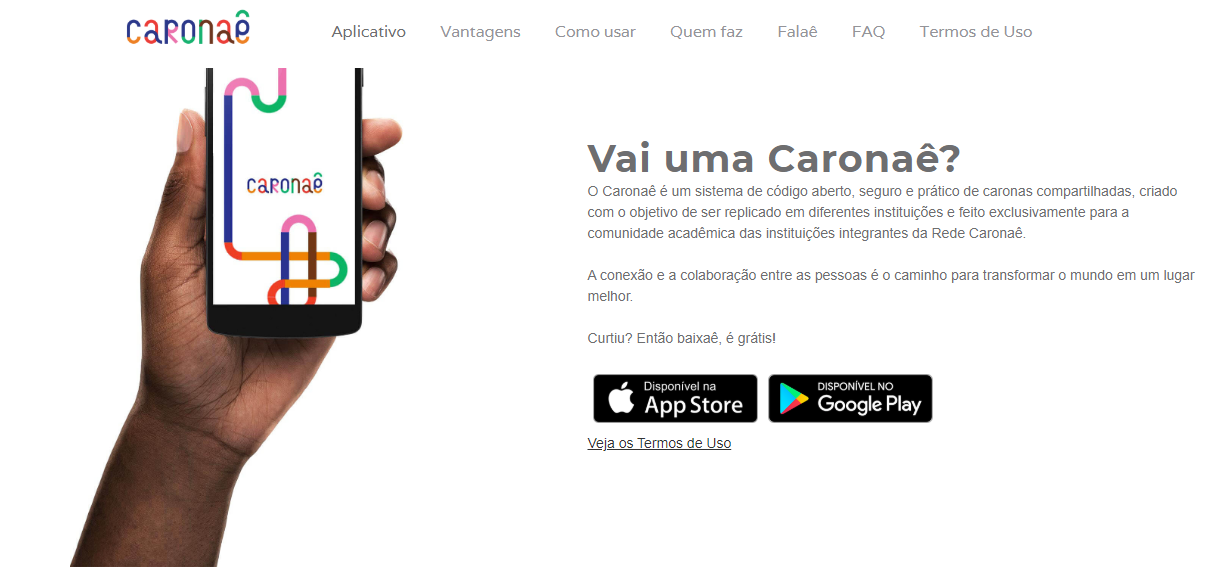
\includegraphics[width=0.8\textwidth]{./04-figuras/caronae.png}
	\label{fig:caronae}
	\fonte{https://caronae.org/index.html}
\end{figure}


%texto escrito por mim

\subsection{Waze Carpool}
Aplicativo das Empresas Waze, o \textit{Waze Carpool} é uma variante dos serviços da Waze que oferece compartilhamento de caronas entre seus usuários. O serviço oferecido pela empresa funciona através de um programa de parcerias. O aplicativo é bem dinâmico e intuitivo. A empresa aproveita os dados do aplicativo Waze para alimentar a dinâmica de navegação do Waze Carpool, como mostra a tela de grupos do aplicativo na Figura~\ref{fig:tela_grupos_wazecarpool}.

\begin{figure}[!hbtp]
	\centering
	\caption{Tela de grupos do aplicativo Waze Carpool}
	
\includegraphics[width=0.25\textwidth]{./04-figuras/waze/Tela_de_grupos.png}
	\label{fig:tela_grupos_wazecarpool}
	\fonte{Programa de Parceria Brasil - Waze Carpool}
\end{figure}

A Waze oferece o serviço do aplicativo para diversas empresas que desejam incorporar a cultura das caronas entre seus empregados porque a empresa acredita que as caronas costumam aproximar mais as pessoas e criar momentos que no local de trabalho não existiriam.

O aplicativo tem uma dinâmica interessante, funciona a partir da criação de grupos, e os usuários destes grupos oferecem caronas entre si. Alunos de universidades como a UFRJ que por um tempo teve o seu próprio aplicativo de carona, o Caronaê, utilizam a ferramenta para pegar e oferecer a carona aos integrantes dos grupos que são criados e gerenciados por uma pessoa que ficar responsável pela comunicação da instituição com a empresa, o chamado "Embaixador".
% texto do material da waze 




\section{Veículos Compartilhados}
Na categoria de veículos compartilhados, separamos dois exemplos dos mais conhecidos com diferentes características cada. Há soluções desde compartilhamentos de bicicletas e automóveis.  %texto escrito por mim

Chips e cartões inteligentes ("\textit{smart-card}") são tecnologias bastante utilizadas nesse tipo de modelo de solução de mobilidade. Os chips utilizados em muitos casos para monitorar as bicicletas compartilhadas, e em algumas cidades, como Rennes na França, em 1998, utilizava os cartões inteligentes para a liberação das bicicletas nas estações.%mestrado da luisa

Aliás, Paris foi uma das primeiras cidades a utilizar os chamados sistemas de terceira geração, no qual a tecnologia utilizada é capaz de controlar o uso dos veículos em tempo real, GPS, cartões inteligentes, chips, todos, entram na lista dos dispositivos que possibilitam esse controle.

\subsection{Yellow}

Utilizando chips em seus veículos e QR Code para desbloquear seus veículos, a Yellow é uma startup brasileira de micromibilidade -- termo dado para veículos que servem para percorrer distâncias curtas -- que aluga bicicletas e partinetes elétricos fundada em 2017. Funcionando através de um serviço \textit{dockless}, ou seja, ao invés das bicicletas terem um ponto de estacionamento especifico, elas podem ser encontradas e deixadas em qualquer lugar que esteja dentro das áreas de atuação exibidas pelo aplicativo, podendo ser monitorada e controlada. 

Após o fim do uso, basta o usuário travar o cadeado que fica na bicicleta, que está pronta para o próximo usuário. A Yellow também utiliza o GPS, tanto para mostrar o trajeto percorrido pelo usuário quanto para apresentar onde estão as bicicletas no mapa. Na figura \ref{fig:yellow-app} é mostrado as áreas de atuação e a localização das bicicletas na cidade de São Paulo.

\begin{comment}
https://tecnoblog.net/286176/como-funciona-o-aluguel-de-bicicletas-e-patinetes-da-yellow/
\end{comment}

\begin{figure}[!hbtp]
	\centering
	\caption{Mapa do aplicativo Yellow na cidade de São Paulo}
	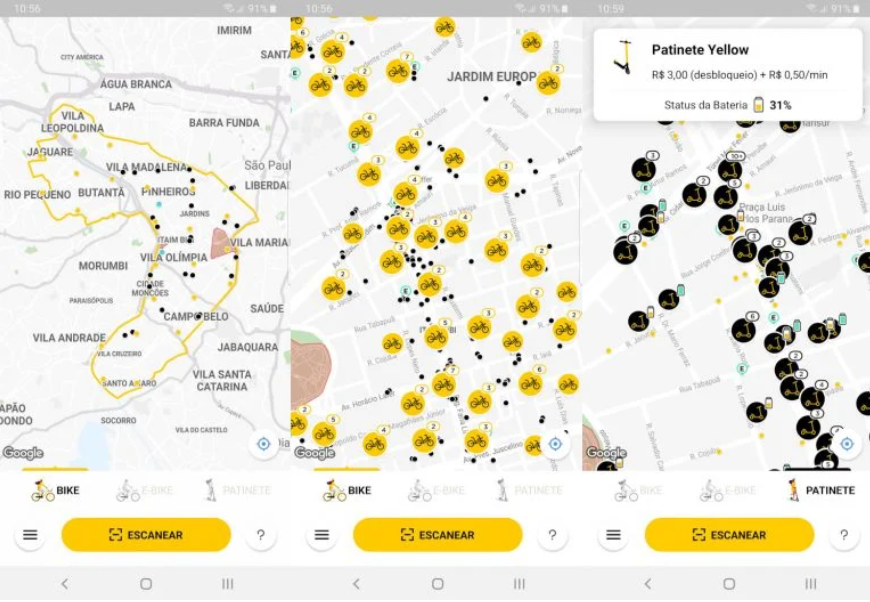
\includegraphics[width=0.6\textwidth]{./04-figuras/yellow/yellow.png}
	\label{fig:yellow-app}
	\fonte{https://tecnoblog.net/286176/como-funciona-o-aluguel-de-bicicletas-e-patinetes-da-yellow/} 
\end{figure}

\subsection{ZipCar}

Utilizando conceitos de \textit{Carsharing}, a empresa norte-americana que ainda não chegou com seus serviços no Brasil utiliza dos seus recursos tecnológicos -- aplicativo para dispositovos móveis -- para compartilhar carros entre seus usuários no estilo B2C (Business-to-Consumer). Semelhante a empresa Yellow, os usuários geralmente conseguem encontrar veículos próximos através de seus dispositivos móveis.

Segundo \cite{ballus-armet} os usuários do Zipcar precisam ao final do uso do veículo, devolvê-lo ao ponto de origem, algo que e chama de \textit{round-trip} ou ida e volta, modelo usado pela Zipcar. Outra empresa semelhante ao Zipcar é a Car2Go, divergindo no modelo de utilizaçao, na Car2Go o usuário deixa o veículo em uma localidade diferente por ser corridas chamadas \textit{one way}, ou seja, trecho único.

Ambos modelos de negócio estão relacionados a economia colaborativa e utilizam a plataforma da Internet, redes sociais, sistemas de informação e recursos tecnológico para oferecer o serviço e conectar seus usuários \cite{ballus-armet}. O aluguel são para pessoas que geralmente precisam de carros por poucas horas, % https://medium.com/@edselferri/o-case-zipcar-a7cbded4ba02#:~:text=Eles%20t%C3%AAm%20uma%20tecnologia%20sem,a%20torna%20um%20neg%C3%B3cio%20%C3%BAnico.
os clientes podem reservar um carro on-line e usar um cartão RFID chamado zipcard para entrar no carro reservado, passando o cartão no leitor perto do pára-brisa do motorista \cite{pearlson2009strategic} %\mnote{é um livro, precisa encontrar a página}.

%https://medium.com/@edselferri/o-case-zipcar-a7cbded4ba02#:~:text=Eles%20t%C3%AAm%20uma%20tecnologia%20sem,a%20torna%20um%20neg%C3%B3cio%20%C3%BAnico.
% texto copiado do site
Além de ter um serviço exclusivo, a Zipcar emprega tecnologia poderosa para dar suporte ao seu modelo de negócios \cite{pearlson2009strategic}. Eles têm uma tecnologia sem fio patenteada que é usada para monitorar a segurança do carro, o nível de feules, o uso por hora e outros recursos \cite{pearlson2009strategic}. A Zipcar desenvolveu um modelo de negócio único e apoiou-a com tecnologia apropriada, o que a torna um negócio único. Na figura \ref{fig:zipcar} mostra um usuário desbloqueando as portas do veículo da Zipcar.

\begin{figure}[!hbtp]
	\centering
	\caption{Como desbloquear seu Zipcar}
	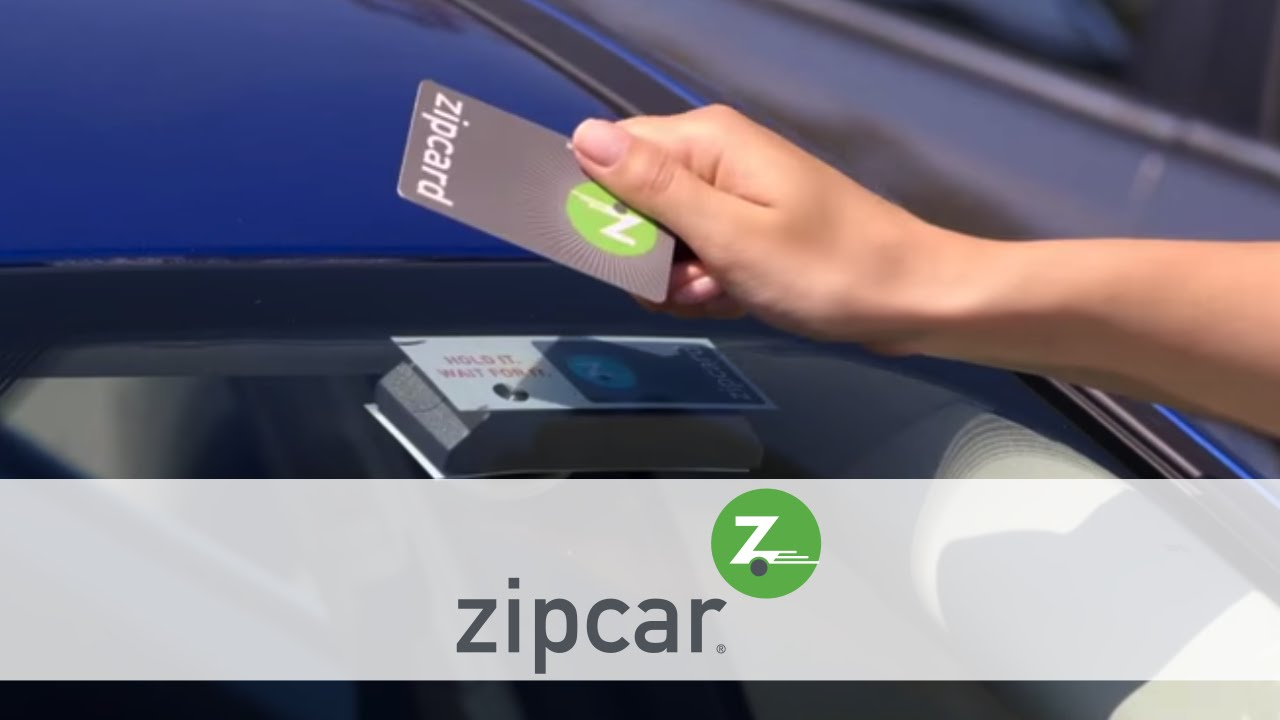
\includegraphics[width=0.8\textwidth]{./04-figuras/zipcar/zipcar.jpg}
	\label{fig:zipcar}
	\fonte{https://money.usnews.com/money/business-economy/articles/2008/06/05/5-keys-to-zipcars-success} %acesso: 13/04/2021 
\end{figure}


\begin{comment}
\section{Quadro Comparativo entre as soluções}
Depois de mostrar algumas das soluções existentes de mobilidade inteligente ao redor do mundo, vamos realizar uma comparação de qual solução será mais viável de ser implementada na Unifap levando em consideração o contexto local, as dificuldades de implementação e o questionário respondido pelo corpo docente e discente do Campus Macapá.

Levando em consideração o questionário que foi aplicado,logo de inicio, descartamos soluções de mobilidade inteligente que tem fins lucrativos e comerciais, como "Transporte Individual Privativo de Passageiros", além de não oferecerem nenhum serviço para o objetivo aqui proposto. Também, as "Orientações de Mobilidade" foram mencionadas para explanar sobre o tipo de mobilidade inteligente, porém, foge da ideia do projeto, pois não conseguiríamos oferecer o mínimo de garantia de segurança, praticidade e conforto.

As demais categorias mencionadas, "Viagens Compartilhadas" e "Veículos Compartilhados" foram analisados, e concluímos que seriam as mais viáveis. Excluímos as soluções privadas, que não garantiriam alguns requisitos mencionados no formulário, e analisamos 3 opções para oferecer, bicicletas compartilhadas, da categoria de veículos compartilhados e 2 soluções da categoria compartilhamento de corridas, Waze Carpool e Caronaê.

Os critérios foram baseados em cima das complexidade e contratempos que poderiam ter durante o processo de implementação, consideramos a infraestrutura institucional (UNIFAP) e da cidade de Macapá. Levamos em consideração também o custo tanto pro usuário, quanto pra universidade em organizar, gerenciar e manter os serviços da solução, além de necessidade futura de estar preparada para oferecer o serviço com qualidade independente do volume de dados. Soluções que já dispõem sua própria infraestrutura tecnológica parece atraente, porém, a maioria não fica dentro dos requisitos da comunidade da Unifap.

No quadro \ref{tab:quadro-solusdemobilidade} resume as características e modelos de negócios citados, apresentando algumas funcionalidades e regra de negócio de cada solução, além de expor quais soluções estão disponíveis para uso conforme as necessidades locais. O aplicativo Caronaê aparece como opção por ser de código aberto, e disponibiliza pelo GitHub a plataforma mobile, sua área administrativa e demais serviços, já o Waze Carpool nos da a possibilidade de criar grupos fechados, nos da todo o aparato tecnologico e as aplicações, nos dando apenas a responsabilidade de gerenciar os usuários e grupos. 
% Please add the following required packages to your document preamble:
% \usepackage{graphicx}
% \usepackage[table,xcdraw]{xcolor}
% If you use beamer only pass "xcolor=table" option, i.e. \documentclass[xcolor=table]{beamer}
% \usepackage{lscape}

\begin{landscape}
\begin{quadro}[]
\caption{Soluções de mobilidade}
\label{tab:quadro-solusdemobilidade}
\resizebox{1.5\textwidth}{!}{%
\begin{tabular}{|l|l|l|l|l|l|l|l|l|l|l|l|}
\hline
\multicolumn{12}{|c|}{Soluções de mobilidade} \\ \hline
\multicolumn{1}{|c|}{Nome} &
  Categoria &
  \multicolumn{1}{c|}{\begin{tabular}[c]{@{}c@{}}Oferecer/Solicitar\\ Caronas\end{tabular}} &
  \multicolumn{1}{c|}{Proprietário} &
  \multicolumn{1}{c|}{\begin{tabular}[c]{@{}c@{}}Ambiente\\ administrativo \\ disponível a terceiros\end{tabular}} &
  \multicolumn{1}{c|}{Autenticação} &
  \multicolumn{1}{c|}{GPS} &
  \multicolumn{1}{c|}{\begin{tabular}[c]{@{}c@{}}Utiliza remuneração\\ no aplicativo\end{tabular}} &
  Plataforma &
  \begin{tabular}[c]{@{}l@{}}Identificação do \\ usuário\end{tabular} &
  Código aberto &
  Infraestrutura \\ \hline
Waze &
  \begin{tabular}[c]{@{}l@{}}Orientação \\ de mobilidade\end{tabular} &
  Não &
  Waze Mobile &
  Não &
  \begin{tabular}[c]{@{}l@{}}Qualquer pessoa \\ que realizar o cadastro\end{tabular} &
  {\color[HTML]{000000} Sim} &
  Não &
  Android IOS &
  Conta cadastrada &
  Não &
  Própria \\ \hline
Cittamobi &
  \begin{tabular}[c]{@{}l@{}}Orientação \\ de mobilidade\end{tabular} &
  Não &
  Cittati &
  Não &
  \begin{tabular}[c]{@{}l@{}}Qualquer pessoa \\ que realizar o cadastro\end{tabular} &
  Sim &
  Não &
  Android IOS &
  Conta cadastrada &
  Não &
  Própria \\ \hline
Moovit &
  \begin{tabular}[c]{@{}l@{}}Orientação \\ de mobilidade\end{tabular} &
  Não &
  Moovit Inc. &
  Não &
  \begin{tabular}[c]{@{}l@{}}Qualquer pessoa \\ que realizar o cadastro\end{tabular} &
  Sim &
  Não &
  Android IOS &
  Conta cadastrada &
  Não &
  Própria \\ \hline
Google Maps &
  \begin{tabular}[c]{@{}l@{}}Orientação \\ de mobilidade\end{tabular} &
  Não &
  Google &
  Não &
  \begin{tabular}[c]{@{}l@{}}Qualquer pessoa \\ que realizar o cadastro\end{tabular} &
  Sim &
  Não &
  Android IOS &
  Conta cadastrada &
  Não &
  Própria \\ \hline
Uber &
  \begin{tabular}[c]{@{}l@{}}Transporte índividual\\ privado de passageiros\end{tabular} &
  Não &
  Uber Technologies Inc. &
  Não &
  \begin{tabular}[c]{@{}l@{}}Qualquer pessoa \\ que realizar o cadastro\end{tabular} &
  Sim &
  Sim &
  Android IOS &
  Conta cadastrada &
  Não &
  Própria \\ \hline
99 &
  \begin{tabular}[c]{@{}l@{}}Transporte índividual\\ privado de passageiros\end{tabular} &
  Não &
  Didi Chuxing &
  Não &
  \begin{tabular}[c]{@{}l@{}}Qualquer pessoa \\ que realizar o cadastro\end{tabular} &
  Sim &
  Sim &
  Android IOS &
  Conta cadastrada &
  Não &
  Própria \\ \hline
Blablacar &
  Viagens compartilhadas &
  Sim &
  Comuto SA &
  Não &
  \begin{tabular}[c]{@{}l@{}}Qualquer pessoa \\ que realizar o cadastro\end{tabular} &
  Não &
  Sim &
  Android IOS &
  Conta cadastrada &
  Não &
  Própria \\ \hline
Yellow &
  Veículos compartilhados &
  Não &
  Grow &
  Não &
  \begin{tabular}[c]{@{}l@{}}Qualquer pessoa \\ que realizar o cadastro\end{tabular} &
  Sim &
  Sim &
  Android IOS &
  Conta cadastrada &
  Não &
  Própria \\ \hline
Cabify &
  Viagens compartilhadas &
  Não &
  Juan de Antonio &
  Não &
  \begin{tabular}[c]{@{}l@{}}Qualquer pessoa \\ que realizar o cadastro\end{tabular} &
  Sim &
  Sim &
  Android IOS &
  Conta cadastrada &
  Não &
  Própria \\ \hline
Bynd &
  Viagens compartilhadas &
  Não &
   &
  Não &
  \begin{tabular}[c]{@{}l@{}}Qualquer pessoa \\ que realizar o cadastro\end{tabular} &
  Sim &
  Sim &
  Android IOS &
  Conta cadastrada &
  Não &
  Própria \\ \hline
Vemcar &
  Viagens compartilhadas &
  Sim &
  UFMG &
  Não &
  \begin{tabular}[c]{@{}l@{}}Somente alunos da \\ UFMG\end{tabular} &
  Sim &
  Recompensas &
  Android &
  \begin{tabular}[c]{@{}l@{}}Sistema de Gestão\\ da UFMG\end{tabular} &
  Não &
  UFMG \\ \hline
ZipCar &
  Veículos compartilhados &
  Não &
  Avis Budget Group &
  Não &
  \begin{tabular}[c]{@{}l@{}}Qualquer pessoa \\ que realizar o cadastro\end{tabular} &
  Sim &
  Sim &
  Android IOS &
  Conta cadastrada &
  Não &
  Própria \\ \hline
Caronaê &
  Viagens compartilhadas &
  Sim &
  UFRJ &
  Sim &
  \begin{tabular}[c]{@{}l@{}}Somente alunos da \\ UFRJ\end{tabular} &
  Não &
  Não &
  Android IOS &
  \begin{tabular}[c]{@{}l@{}}Sistema de Gestão \\ da UFRJ\end{tabular} &
  %\cellcolor[HTML]{FFFC9E}
  Sim &
  UFRJ \\ \hline
Waze Carpool &
  Viagens compartilhadas &
  Sim &
  Waze Mobile &
  %\cellcolor[HTML]{FCFF2F}
  Sim &
  \begin{tabular}[c]{@{}l@{}}Qualquer pessoa \\ que realizar o cadastro\end{tabular} &
  Sim &
  Sim &
  Android IOS &
  Conta cadastrada &
  Não &
  Própria \\ \hline
\end{tabular}%
}
\end{quadro}
\end{landscape}


%%%%%%%%%5
\begin{comment}
	\mnote{Patrícia: vais ter que expandir esse capítulo. Se nao me engano a gnt tnha conversado sobre falar de algumas soluções de mobilidade inteligente existentes, vai ser importante para o teu argumento. Vou criar uma seção somente para "veículos compartilhados", ou seja, app de carona, uber, etc, depois vc organiza e vê se é o melhor termo e cria as demais seções.}
    %
    
    %
	\mnote{Patrícia: vamos pensar se colocamos essa seção na próxima seção de proposta e resultados preliminares.}
    %
\end{comment}
%%%%%%%%
\end{comment}


   	%
% Documento: Proposta
%


%\chapter{Proposta e Resultados Preliminares}\label{chap:proposta}  
\chapter{Carona solidária para Unifap}\label{chap:Carona solidária para Unifap}  

\section{Perfil da comunidade acadêmica e os problema enfrentados}

%Na pesquisa realizada para o projeto entre os meses 05/2019 à 11/2019, os entrevistados (comunidade acadêmica) responderam a seguinte pergunta: \textit{“Qual(is) os motivos já fez(fizeram) você deixar de ir à Universidade?”} e colocamos como opção alguns motivos que podem ter sido os causados, \textit{“Por falta de dinheiro”}, \textit{“Por problemas com chuva”, "Por problemas com o transporte público”}, \textit{“Deslocamento difícil entre casa e Universidade”}, e tivemos como o maior motivo o \textit{“Problemas com o transporte público”}, é possível ver isso na Figura~\ref{fig:dadosmeiodetransporte}
Na pesquisa realizada para o projeto entre os meses de 05/2019 e 11/2019, os entrevistados responderam à seguinte pergunta: \textit{“Quais os motivos que o levaram a deixar de ir para a faculdade?"} e demos como opção alguns motivos que poderiam ser responsáveis, \textit{"Por falta de dinheiro"}, \textit{"Problemas com a chuva"}, \textit{"Problemas com transporte público"}, \textit{"Dificuldade de deslocamento entre casa e faculdade"}, e tivemos como maior motivo problemas com transporte público. Vejamos o resultado a pergunta na figura ~\ref{fig:dadosmeiodetransporte}.




\begin{figure}[!hbtp]
	\centering
	\caption{Pergunta sobre os motivos que fizeram os alunos não comparecerem a universidade.}
	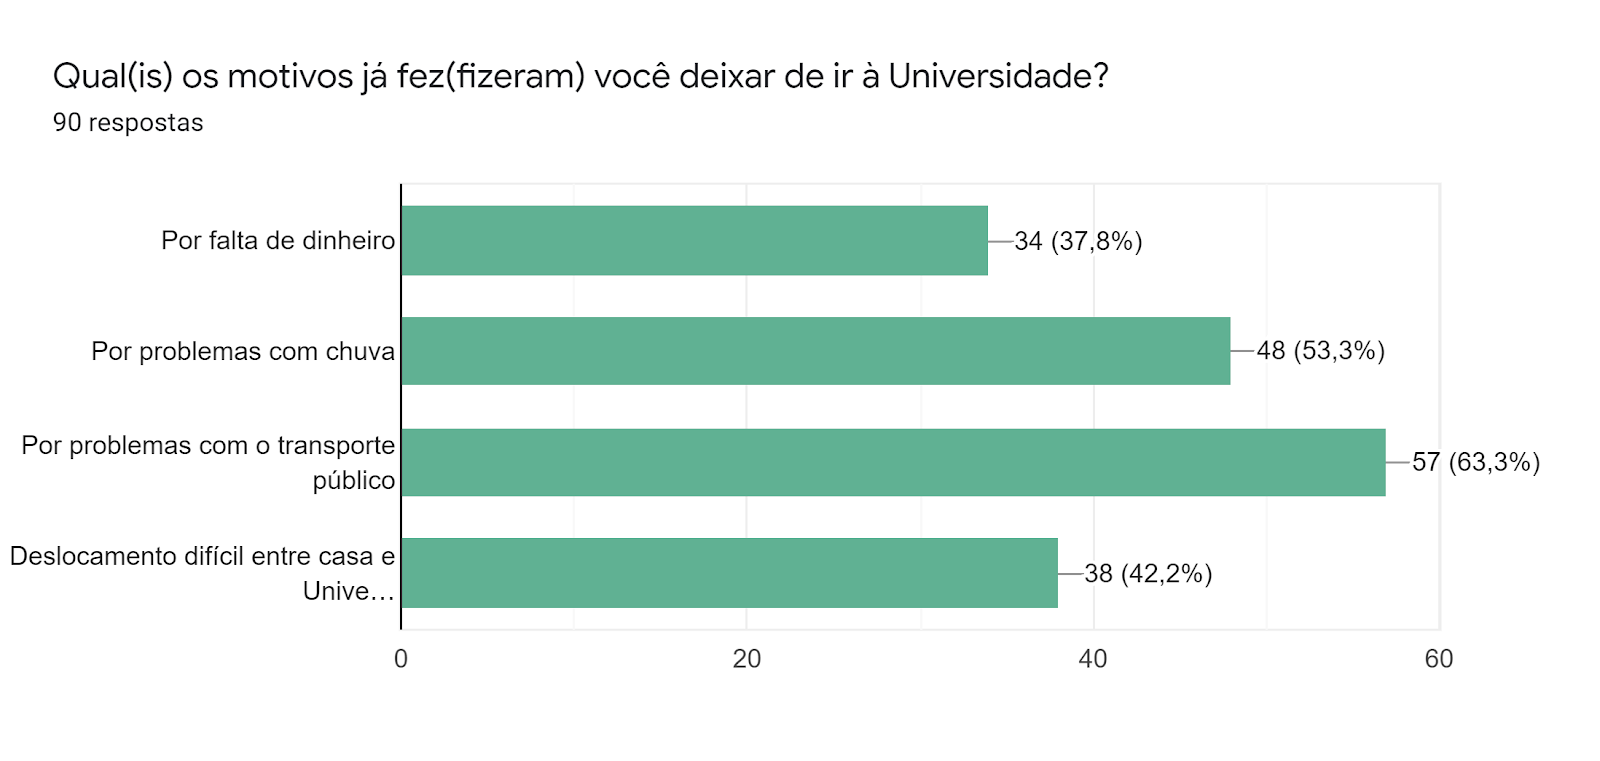
\includegraphics[width=1.0\textwidth]{./04-figuras/questionario/1.png}
	\label{fig:dadosmeiodetransporte}
	\fonte{Elaborado pelo autor.}
\end{figure}

%Proveniente disso, hoje já existem reflexos de problemas relacionados à mobilidade, meio ambiente, economia, etc., e motivado por isso, que será proposto uma solução relacionada à mobilidade inicialmente.
Como resultado, hoje já existem considerações de problemas relacionados à mobilidade, meio ambiente, economia, etc., que levam à proposta de uma solução relacionada primeiramente à mobilidade.

%\section{Resultados do questionário}

%Foi elaborado um questionário com 16 perguntas e obteve 186 respostas, com o objetivo de saber mais sobre a comunidade acadêmica, entre elas, perguntas sobre o sexo, se possui veículo, em qual período que frequenta a universidade, e quantidade de dias que frequenta, todas para entender melhor o perfil e a possibilidade do projeto se encaixar no ambiente universitário, como mostra a \ref{fig:genero}.
Para conhecer melhor a comunidade acadêmica, foi elaborado um questionário de 16 perguntas e recebidas 186 respostas. Isso incluiu perguntas sobre gênero, se possui veículo, quando frequenta a faculdade e quantos dias está lá para entender melhor o perfil e a possibilidade de o projeto se encaixar no ambiente universitário.

\begin{figure}[!hbtp]
	\centering
	\caption{Gênero dos entrevistados}
	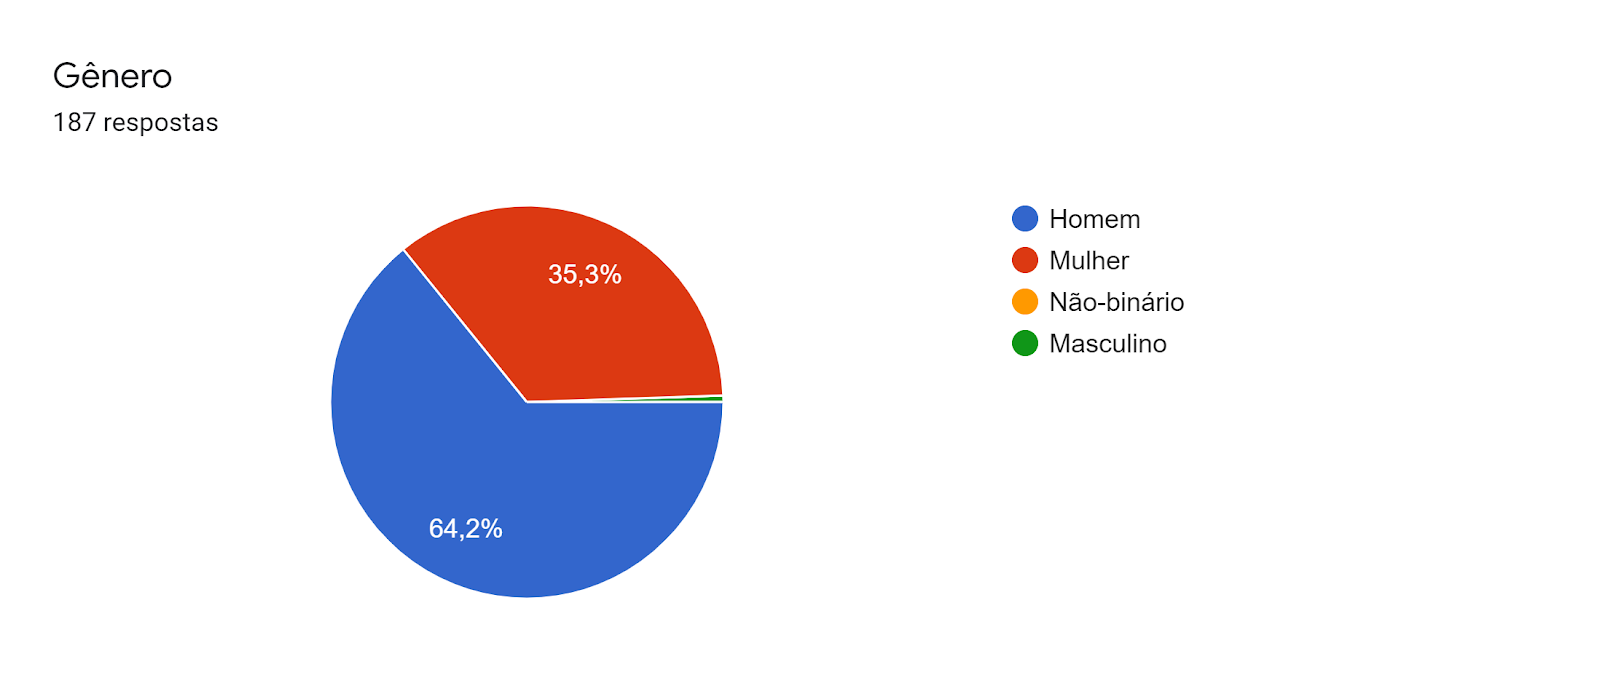
\includegraphics[width=0.8\textwidth]{./04-figuras/questionario/2.png}
	\label{fig:genero}
	\fonte{Elaborado pelo autor.}
\end{figure}

%Foi possível verificar, analisando os resultados do questionário, quais seriam os empecilhos a adesão do projeto, e há uma rejeição em relação a segurança do transporte, principalmente pelas mulheres, que fazem parte de 35,3\% dos entrevistados, possível ver isso na Figura~\ref{fig:aceitacaopelascaronas} e Figura~\ref{fig:aceitacaopelascaronas2}%.
Ao analisar os resultados do questionário, foi possível identificar os obstáculos à participação no projeto. Há uma recusa em relação à segurança viária, principalmente entre as mulheres, que representam 35,3\% dos entrevistados, como você pode ver na Figura~\ref{fig:aceitacaopelascaronas} e Figura~\ref{fig:aceitacaopelascaronas2}%.

\begin{figure}[!hbtp]
	\centering
	\caption{Motivo para aceitar as caronas - Parte 1}
	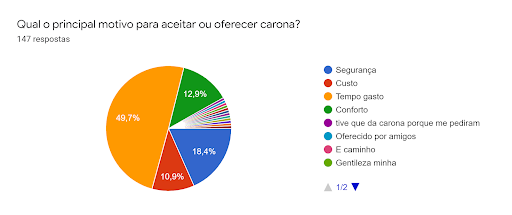
\includegraphics[width=0.7\textwidth]{./04-figuras/questionario/3.png}
	\label{fig:aceitacaopelascaronas}
	\fonte{Elaborado pelo autor.}
\end{figure}

\begin{figure}[!hbtp]
	\centering
	\caption{Motivos para aceitar as caronas - Parte 2}
	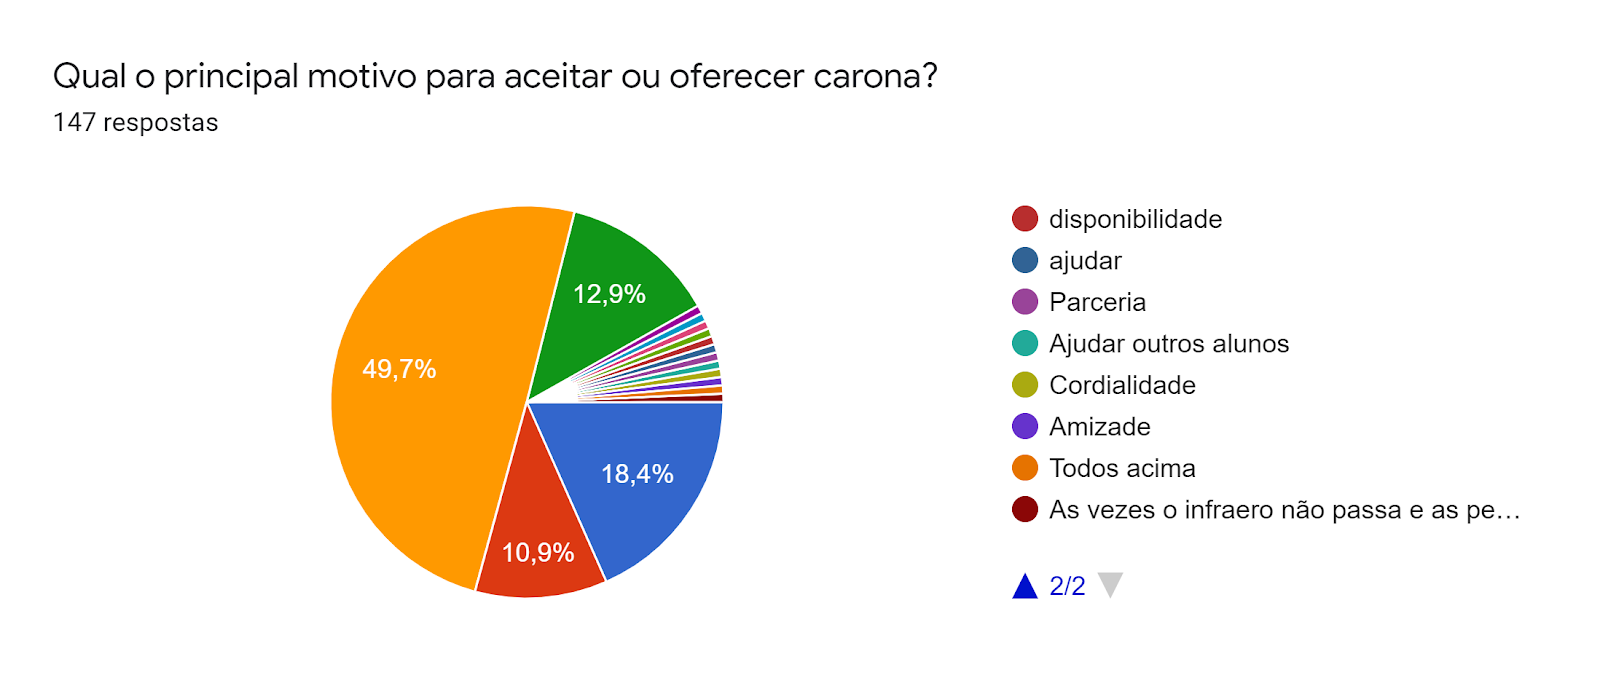
\includegraphics[width=0.7\textwidth]{./04-figuras/questionario/4.png}
	\label{fig:aceitacaopelascaronas2}
	\fonte{Elaborado pelo autor.}
\end{figure}

\mnote{revisar esse techo}
Outros motivos mencionados nesta pergunta foram, \textit{“não ter alguém para oferecer”}, \textit{“falta de oportunidade”}, \textit{“não conheço nenhum aplicativo de carona, motivos que demonstram o interesse da comunidade de receber/oferecer caronas."}

%Pensando nisso, para obter um resultado satisfatório para todos, é pensado algo que foi utilizado em outros projetos relacionados a carona solidária por outras universidades, que é ter como usuários, as pessoas que tem um vínculo ativo com a instituição, utilizando a base de acesso ao sistema da universidade, podendo haver tanto alunos, professores e técnicos como usuários.
Para alcançar um resultado satisfatório para todos, pensa-se em algo que já vem sendo utilizado em outros projetos de caronas em outras universidades, ou seja, ter como usuários pessoas que estejam ativamente conectadas à instituição utilizando a base de acesso ao sistema universitário, estudantes , professores e técnicos, bem como usuários.

Quando questionados sobre a opção do uso exclusivo pelos estudantes, o projeto teve uma grande aceitação por parte da comunidade acadêmica, Figura~\ref{fig:aceitacao}. 

\begin{figure}[!hbtp]
	\centering
	\caption{Pergunta sobre a possibilidade da proposta ser utilizada apenas por pessoas da Unifap}
	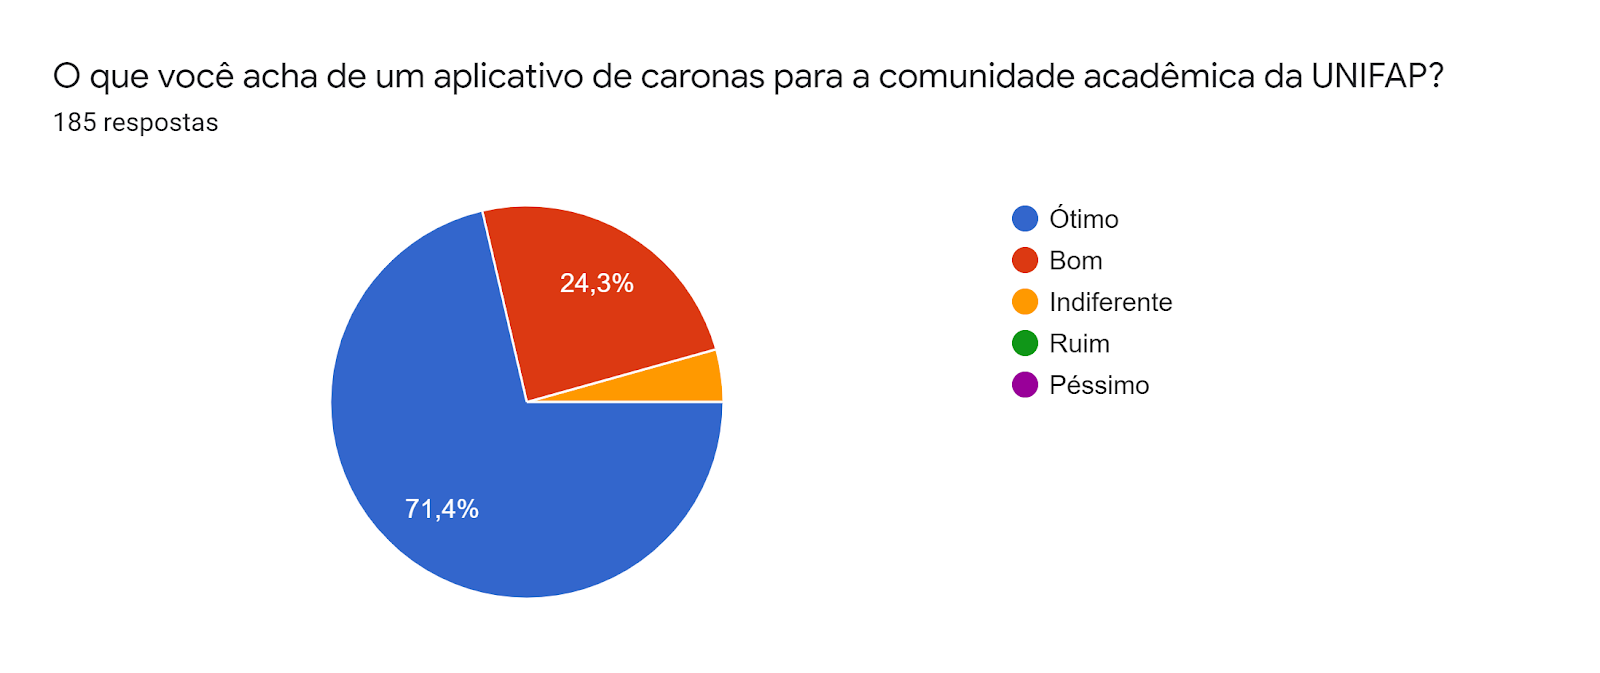
\includegraphics[width=0.7\textwidth]{./04-figuras/questionario/5.png}
	\label{fig:aceitacao}
	\fonte{Elaborado pelo autor.}
\end{figure}

%Pensando no aspecto cultural, será realizado campanhas para incentivar e popularizar o projeto por meio de cartazes espalhados pela universidade, e para melhorar o encontro entre os “caroneiros”, existe a possibilidade de criar pontos de encontros para facilitar mais a vida de quem está disposto a oferecer a carona.
Quanto ao aspecto cultural, serão realizadas campanhas de promoção e divulgação do projeto por meio de cartazes em toda a faculdade. Para melhorar o encontro entre os “caroneiros”, existe a possibilidade de montar pontos de encontro para facilitar a vida de quem se dispuser a oferecer carona.

%A pesquisa deu-se pela pesquisa bibliográfica, estudo de caso e um levantamento de dados por um questionário utilizando a plataforma Google Forms, compreendeu-se que um sistema de caronas para a universidade iria melhorar as condições de mobilidade da instituição e dar outra alternativa ao membro da comunidade acadêmica.
A pesquisa foi realizada por meio de pesquisa bibliográfica, estudo de caso e coleta de dados por meio de questionário utilizando a plataforma Google Forms. Partiu-se do pressuposto de que um sistema de caronas até a faculdade melhoraria as condições de mobilidade da instituição e proporcionaria mais uma alternativa aos membros da comunidade acadêmica.

%Para muitos, o transporte para ir e vir à universidade se torna o grande problema durante a vida acadêmica, tomando um tempo destes para chegar a Universidade e para retornar às suas casas durante os dias letivos, tendo grande espera nas paradas de ônibus, tempo que poderia ser aproveitado para estudar. Mais de 50\% dos entrevistados do formulário responderam que estão insatisfeitos com o transporte que utilizam, isso é apresentado na Figura~\ref{fig:satisfacao}.
Para muitos, o transporte de e para a faculdade torna-se um grande problema durante a vida acadêmica. Levam tempo para chegar à faculdade e voltar para casa durante os dias de aula, e têm que esperar longos períodos nas paradas de ônibus, tempo que poderiam estar usando para estudar. Mais de 50\% dos entrevistados disseram estar insatisfeitos com o transporte que utilizam, conforme mostra a Figura~\ref{fig:satisfacao}

\begin{figure}[!hbtp]
	\centering
	\caption{Pergunta sobre a satisfação dos usuários com o transporte que utiliza}
	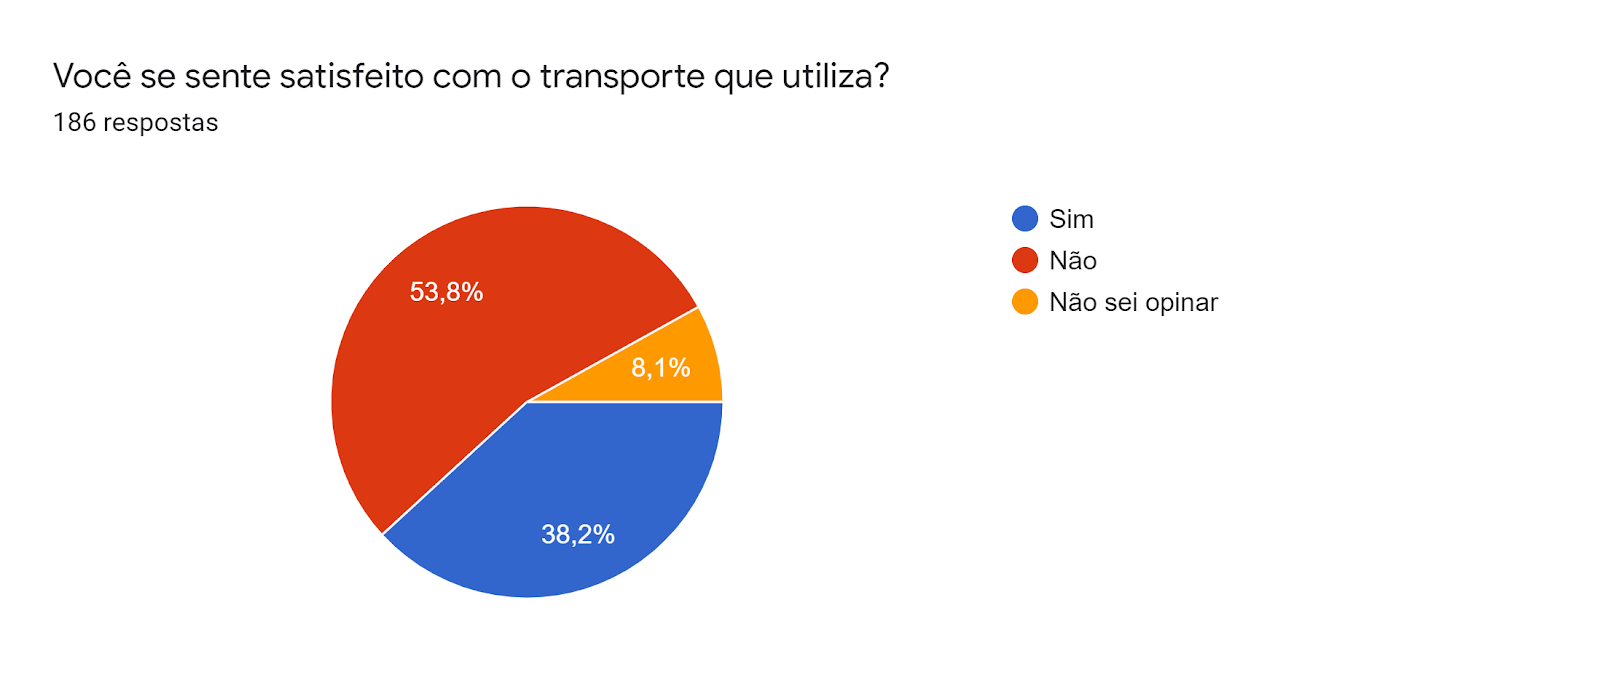
\includegraphics[width=0.7\textwidth]{./04-figuras/questionario/6.png}
	\label{fig:satisfacao}
	\fonte{Elaborado pelo autor.}
\end{figure}

%E mais de 50\% destes entrevistados utilizam o transporte público para chegar ou sair da Universidade, e nessa mesma pergunta conseguimos estimar a quantidade dos entrevistados que possuem carro próprio, 26,9\% responderam que utilizam carro para chegar a universidade e 24,7\% utilizam para sair da Universidade, como mostra a figura \ref{fig:chegadanaunifap1} e \ref{fig:saidadaunifap1}.
E mais de 50\% desses entrevistados usam transporte público para ir ou voltar da faculdade. A mesma pergunta permitiu estimar o número de respondentes que possuem carro próprio: 26,9\% responderam que usam carro para chegar à faculdade e 24,7\% para sair da faculdade, conforme mostram as \ref{fig:chegadanaunifap1} e \ref{fig:saidadaunifap1}.

\begin{figure}[!hbtp]
	\centering
	\caption{Como você geralmente chega na Unifap? -  Parte 1}
	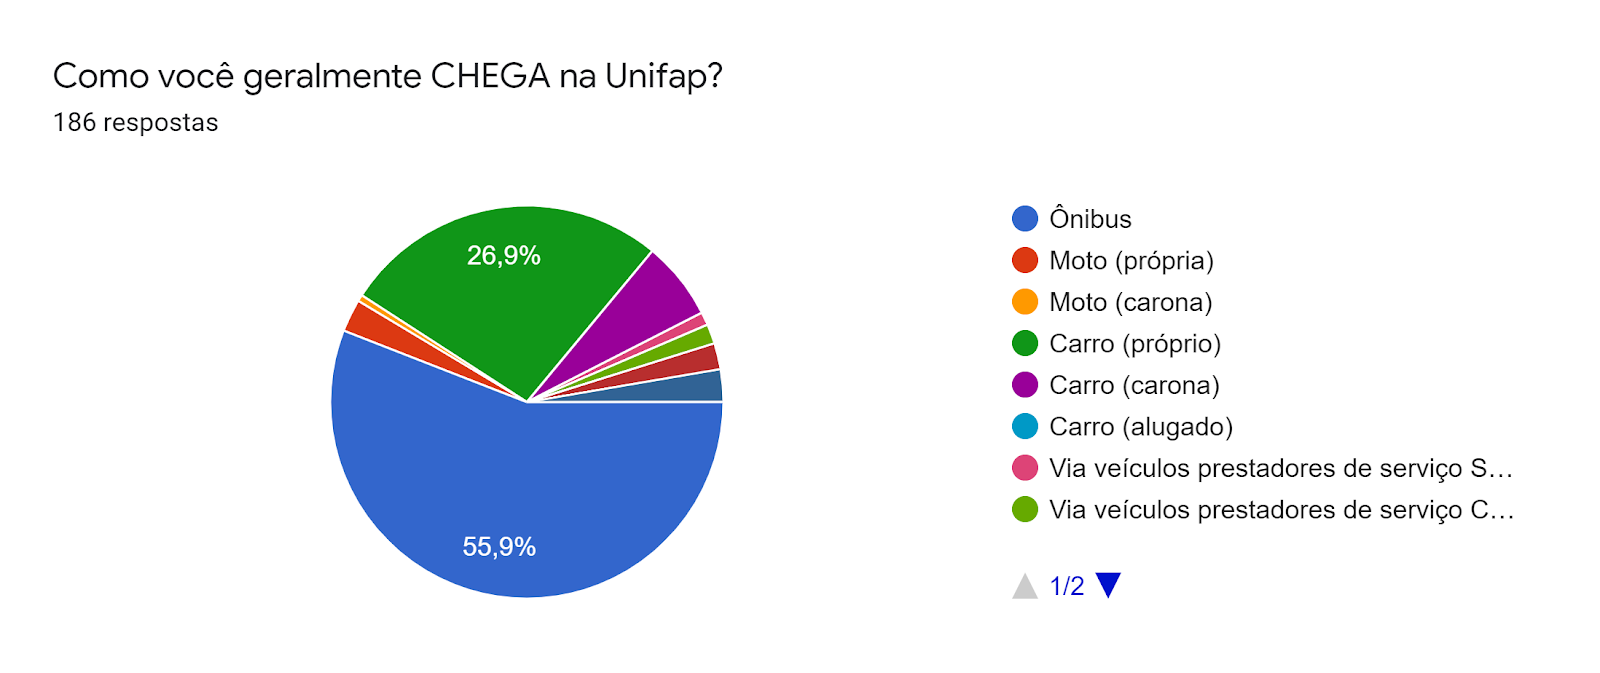
\includegraphics[width=0.6\textwidth]{./04-figuras/questionario/7.png}
	\label{fig:chegadanaunifap1}
	\fonte{Elaborado pelo autor.}
\end{figure}

\begin{comment}
\begin{figure}[!hbtp]
\centering
\caption{Como você geralmente chega na Unifap? - Parte 2}
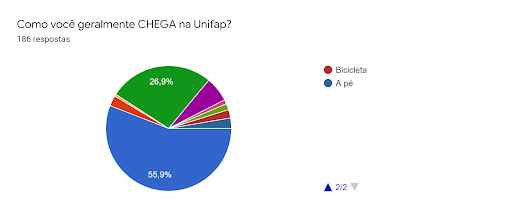
\includegraphics[width=0.6\textwidth]{./04-figuras/questionario/8.png}
\label{fig:chegadanaunifap2}
\fonte{Elaborado pelo autor.}
\end{figure}
\end{comment}


\begin{figure}[!hbtp]
	\centering
	\caption{Como você geralmente sai da Unifap? - Parte 1}
	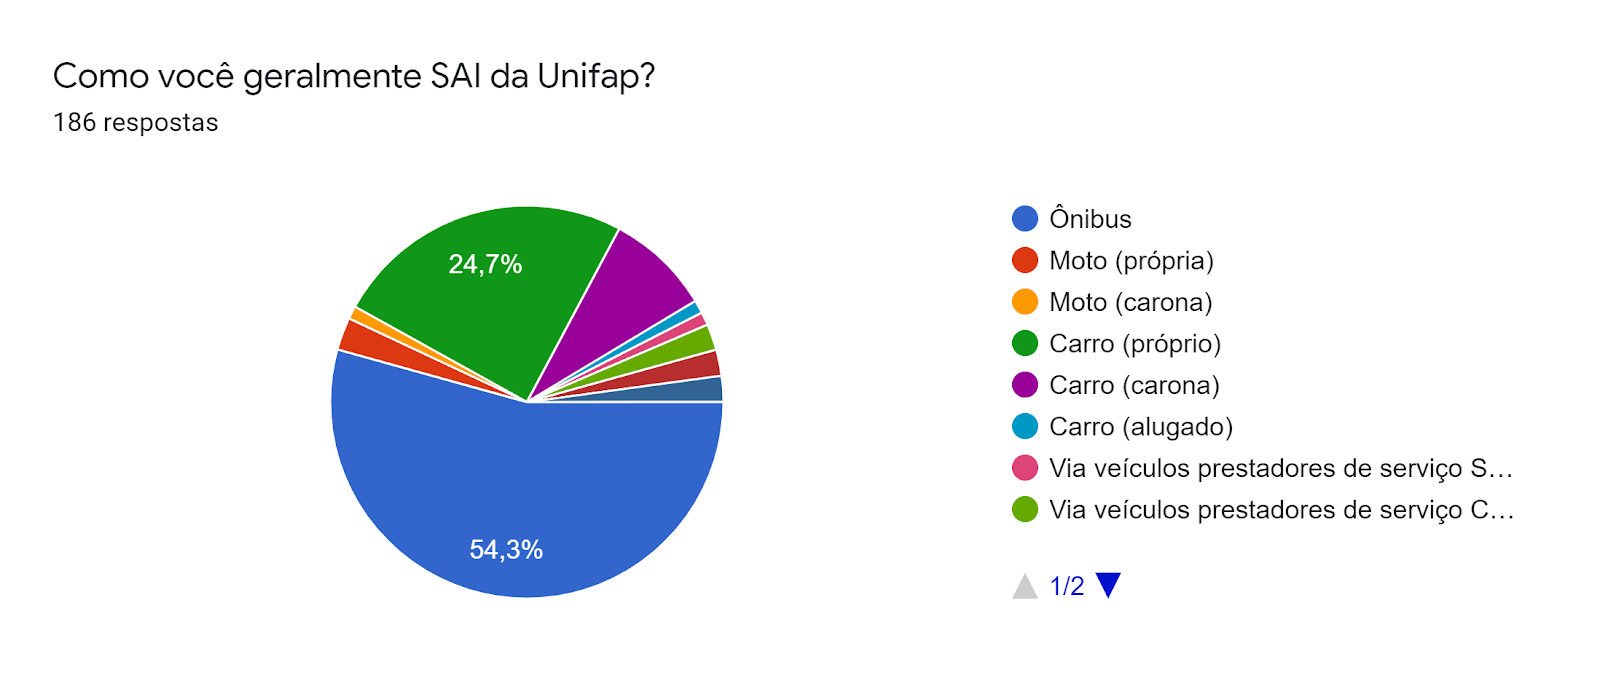
\includegraphics[width=0.6\textwidth]{./04-figuras/questionario/9.png}
	\label{fig:saidadaunifap1}
	\fonte{Elaborado pelo autor.}
\end{figure}

\begin{comment}
	conteúdo...\begin{figure}[!hbtp]
	\centering
	\caption{Como você geralmente sai da Unifap - Parte 2}
	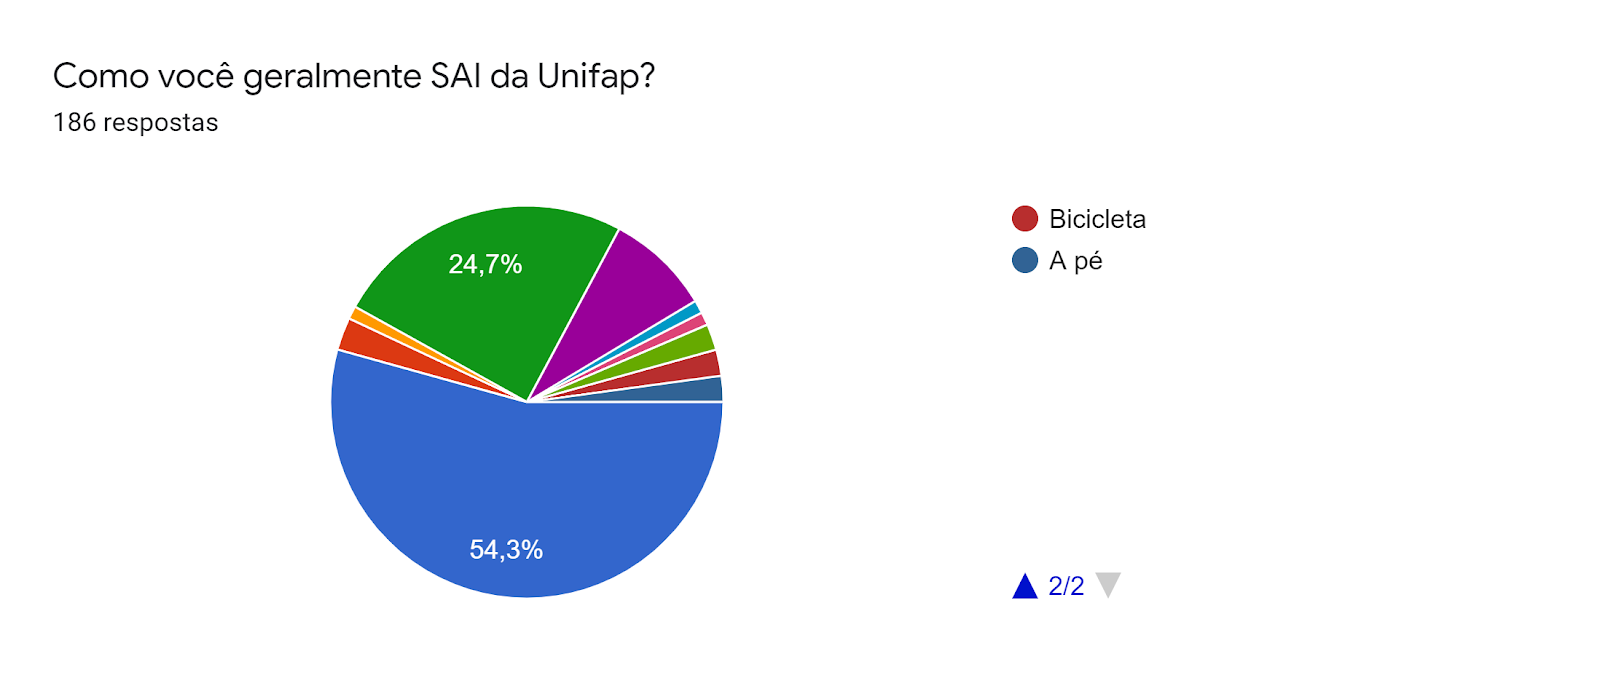
\includegraphics[width=0.6\textwidth]{./04-figuras/questionario/10.png}
	\label{saidadaunifap2}
	\fonte{Elaborado pelo autor.}
	\end{figure}
\end{comment}



%As condições insatisfatórias do sistema de transporte local, além das demoras, superlotação e conforto, os acadêmicos ainda ficam expostos à criminalidade, muitas vezes esperando em paradas escuras durante o período noturno.
As condições insatisfatórias do sistema de transporte coletivo, além de atrasos, superlotação e conforto, os acadêmicos ainda estão expostos à criminalidade e muitas vezes esperam em paradas escuras à noite.

%A maior parte dos acadêmicos apontam como principais problemas, a segurança, o tempo gasto e o conforto que na pesquisa é de suma importância durante o trajeto de ida e volta da universidade. Dos 100 entrevistados que responderam a esta pergunta, 75\% apontam o conforto como um dos problemas, como mostra na figura \ref{fig:problemasenfrentadosparair}.
A maioria dos acadêmicos cita segurança, tempo e conveniência como os principais problemas que são primordiais em pesquisas de ida e volta da faculdade. Dos 100 entrevistados que responderam a essa pergunta, 75\% citam a conveniência como um dos problemas, conforme mostra a \ref{fig:problemasenfrentadosparair}.

\begin{figure}[!hbtp]
	\centering
	\caption{Principais problemas enfrentados com o transporte público local}
	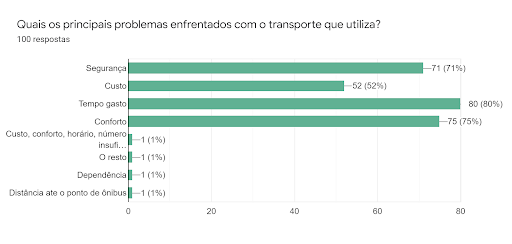
\includegraphics[width=0.6\textwidth]{./04-figuras/questionario/11.png}
	\label{fig:problemasenfrentadosparair}
	\fonte{Elaborado pelo autor.}
\end{figure}


%Na figura \ref{fig:motivos-nao-ir-a-unifao}, das 187 respostas ao questionário, 90 respostas, um pouco menos que 50\% dos entrevistados, responderam quais são os motivos que impedem de ir à universidade, e problemas com o transporte público é o de mais da metade dos que responderam o questionário.
Na Figura \ref{fig:motivos-nao-ir-a-unifao}, das 187 respostas ao questionário, 90 respostas, ou um pouco menos de 50\% dos respondentes, responderam à pergunta sobre quais são os motivos que os impedem de ir à faculdade, e os problemas com transporte público estão em mais metade dos que responderam ao questionário.

\begin{figure}[!hbtp]
	\centering
	\caption{Motivos que já fizeram alunos deixarem de ir a Universidade}
	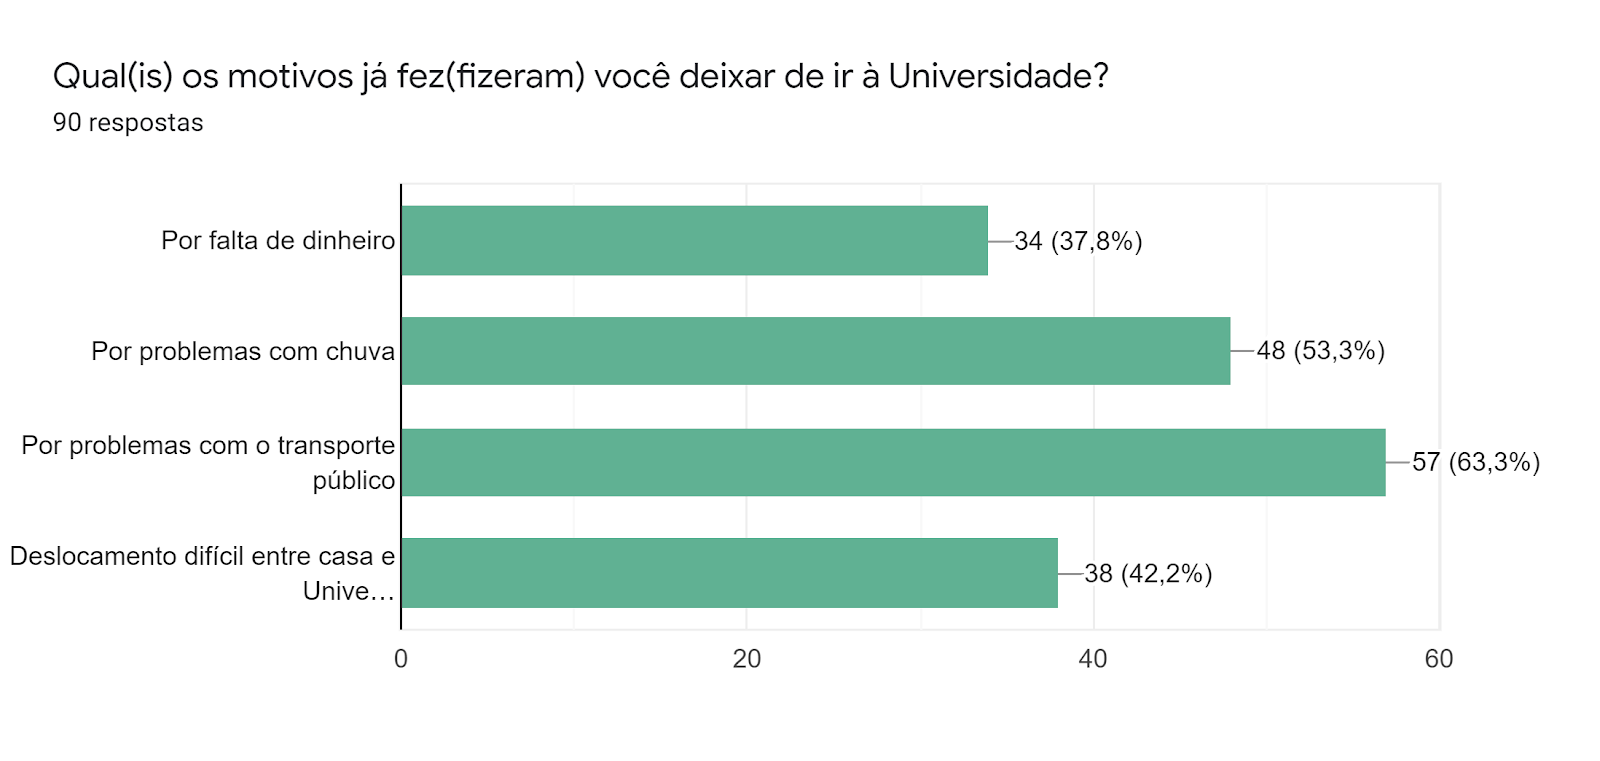
\includegraphics[width=0.6\textwidth]{./04-figuras/questionario/12.png}
	\label{fig:motivos-nao-ir-a-unifao}
	\fonte{Elaborado pelo autor.}
\end{figure}

%Sobre as relações com o tempo gasto, não pararam de ser mencionadas, quando perguntados quais os motivos de aderirem um sistema de caronas, a maioria dos entrevistados apontaram também o tempo gasto como motivo para aceitar caronas, dados apresentados nas figuras \ref{fig:motivosparacarona1} e \ref{fig:motivosparacarona2}.
Quanto à conexão com o gasto de tempo, isso foi mencionado repetidamente. Quando questionados sobre os motivos para participar de uma carona, a maioria dos entrevistados também citou o tempo como motivo para aceitar carona, conforme mostram os dados das figuras \ref{fig:motivosparacarona1} e \ref{fig:motivosparacarona2}.

\begin{figure}[!hbtp]
	\centering
	\caption{Motivos para aceitar carona - Parte 1}
	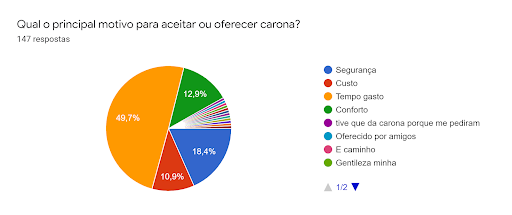
\includegraphics[width=0.7\textwidth]{./04-figuras/questionario/13.png}
	\label{fig:motivosparacarona1}
	\fonte{Elaborado pelo autor.}
\end{figure}

\begin{figure}[!hbtp]
	\centering
	\caption{Motivos para aceitar carona - Parte 2}
	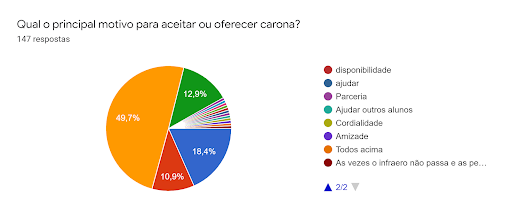
\includegraphics[width=0.7\textwidth]{./04-figuras/questionario/14.png}
	\label{fig:motivosparacarona2}
	\fonte{Elaborado pelo autor.}
\end{figure}

%Quando foi perguntado aos entrevistados se participavam de grupos de caronas, 96,6\% responderam à pesquisa que \textit{“Não participavam”}. Então, um aplicativo de caronas para a universidade poderá criar uma cultura que ainda é inexistente.
Quando perguntados se participam de caronas, 96,6\% dos entrevistados responderam \textit{“Não participavam”}. Assim, um aplicativo de carona na faculdade poderia criar uma cultura que ainda não está presente.

%Das 185 pessoas que responderam o questionário, 97.7\% dos entrevistados acharam \textit{“ótima”} ou \textit{“boa”} a iniciativa de um aplicativo que os usuários possam consultar viagens de ida para a universidade ou de volta da universidade, como mostra na figura \ref{fig:percepcao}.
Das 185 pessoas que responderam ao questionário, 97,7\% dos entrevistados acharam “ótima” ou “boa” a iniciativa de um aplicativo que os usuários podem consultar na ida e volta da faculdade, como mostra a Figura \ref{fig:percepcao}.
\begin{figure}[!hbtp]
	\centering
	\caption{Percepção sobre a proposta de um aplicativo de carona para a Unifap}
	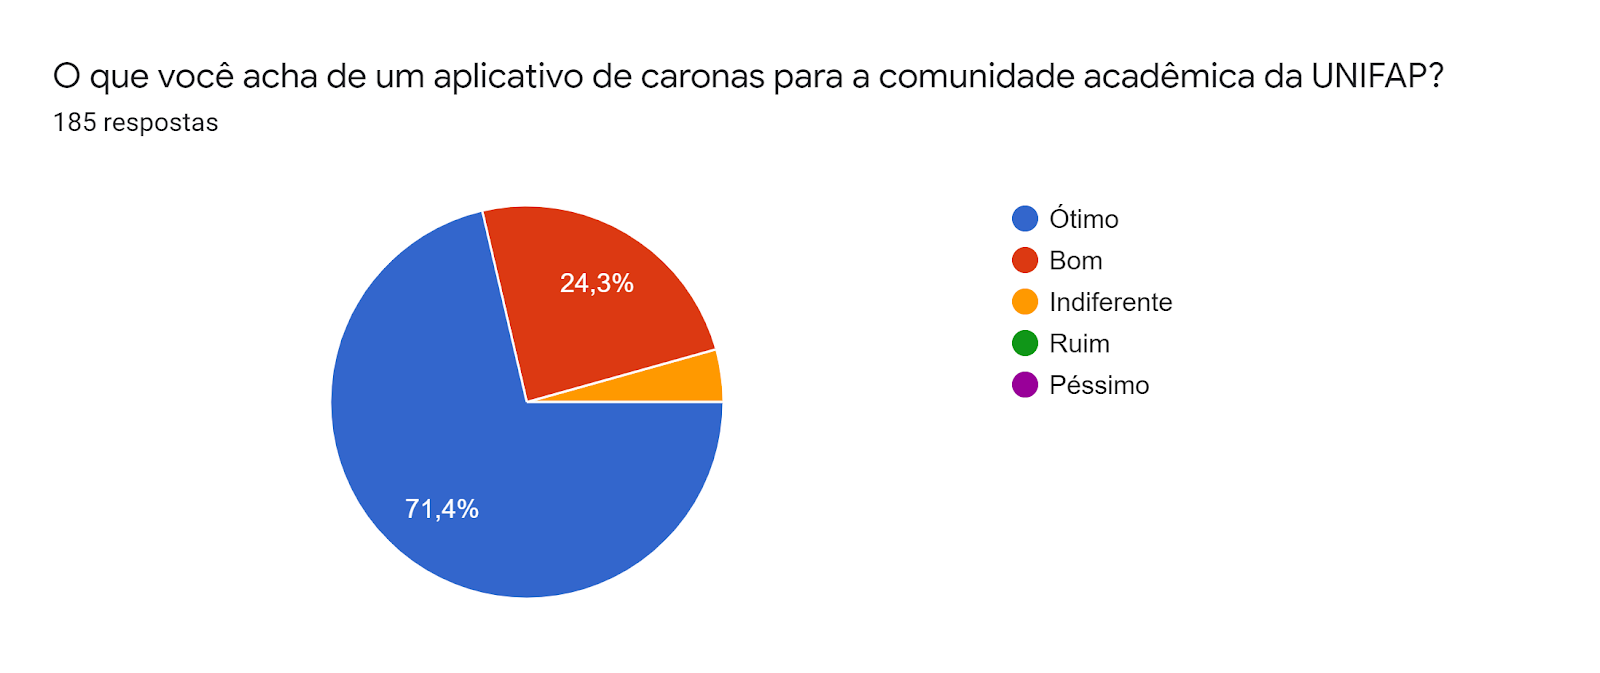
\includegraphics[width=0.7\textwidth]{./04-figuras/questionario/15.png}
	\label{fig:percepcao}
	\fonte{Élaborado pelo autor.}
\end{figure}

%Em relação a esse uso de tecnologia, a comunidade acadêmica já está bem familiarizada com aplicativos relacionados à mobilidade, na figura \ref{fig:conhecimento-sobre-apps}, das 186 respostas ao questionário, apenas 15,1\% responderam não utilizar nenhum dos aplicativos listados.
Em termos de uso de tecnologia, a comunidade acadêmica já está bem versada em aplicações relacionadas à mobilidade. Na Figura \ref{fig:conhecimento-sobre-apps}, das 186 respostas ao questionário, apenas 15,1\% indicaram não utilizar nenhum dos aplicativos listados.

\begin{figure}[!hbtp]
	\centering
	\caption{Percepção sore o conhecimento e uso de tecnologias similares a proposta}
	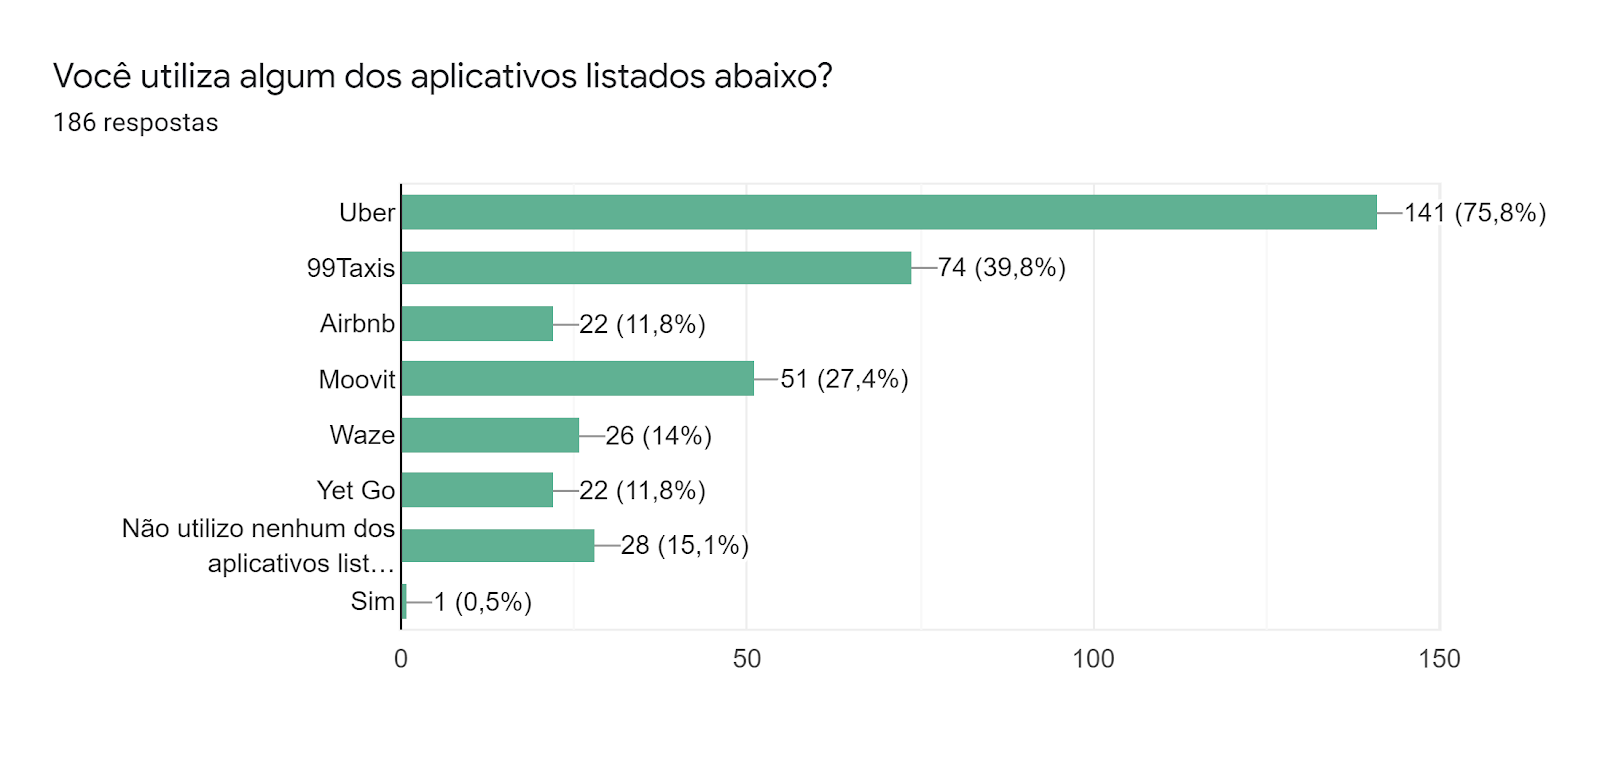
\includegraphics[width=0.7\textwidth]{./04-figuras/questionario/16.png}
	\label{fig:conhecimento-sobre-apps}
	\fonte{Elaborado pelo autor.}
\end{figure}

%No questionário, foi verificado o tempo gasto pela comunidade utilizando smartphones, dispositivo necessáriao para o uso do aplicativo, e apenas 1,6\% dos entrevistados informaram que não possuem smartphones, e 37\% passam mais de 6h utilizando os dispositivos diariamente, como mostra na figura \ref{fig:usodosmartphone}.
O questionário revisou o tempo que a comunidade gasta usando smartphones, um dispositivo necessário para o uso do aplicativo. Apenas 1,6\% dos entrevistados informaram que não possuem smartphones e 37\% passam mais de 6 horas por dia usando os dispositivos, conforme mostra a Figura \ref{fig:usodosmartphone}.

\begin{figure}[!hbtp]
	\centering
	\caption{Tempo de uso do \textit{Smartphone} pelos entrevistados}
	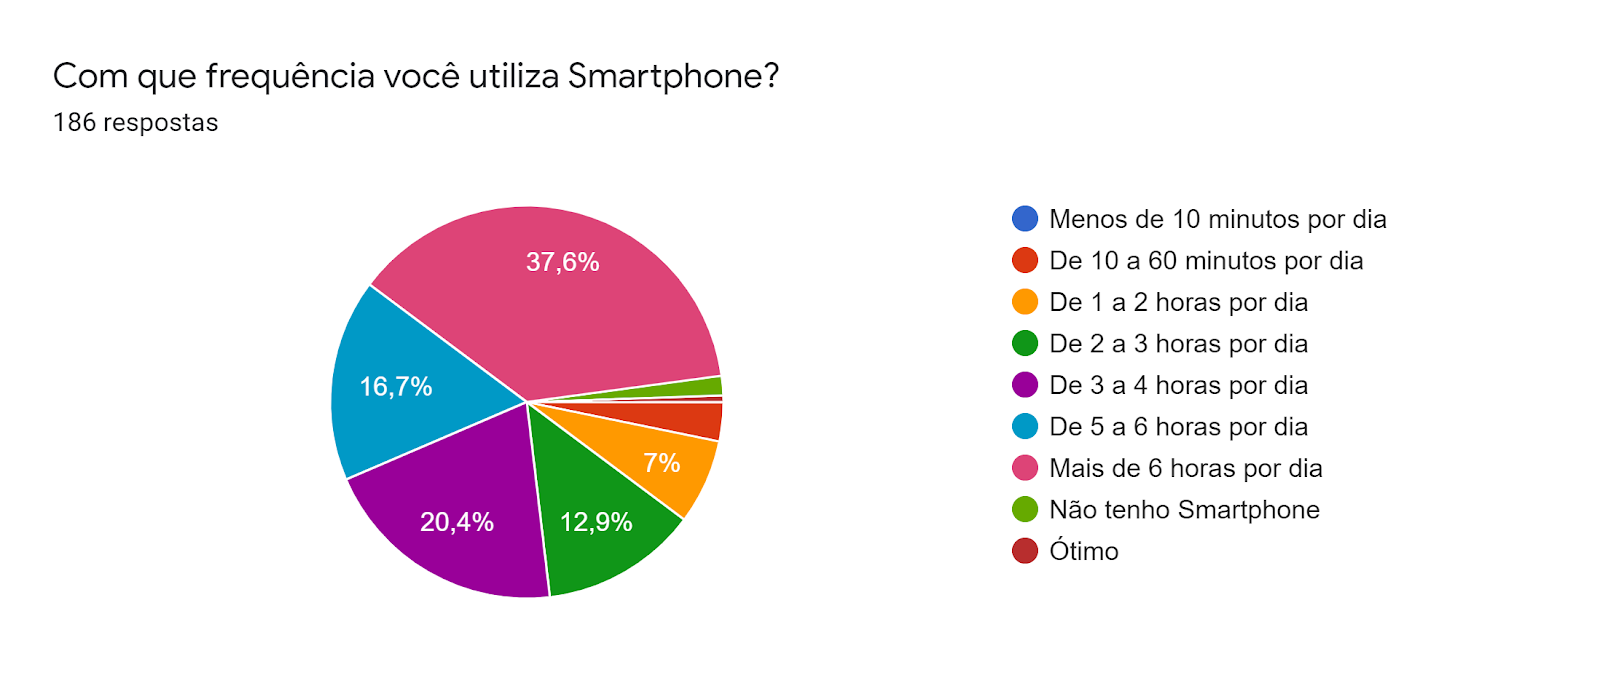
\includegraphics[width=0.7\textwidth]{./04-figuras/questionario/17.png}
	\label{fig:usodosmartphone}
	\fonte{Elaborado pelo autor}
\end{figure}

%O resultado foi satisfatório, percebe-se que a comunidade está disposta a aderir a proposta do aplicativo de carona solidária, onde muitos se interessam em oferecer ou receber carona. 
%porém, falta algo que auxilie-os.
O resultado foi satisfatório. Fica claro que a comunidade está disposta a aderir à proposta de carona, pois muitos estão interessados em oferecer ou receber carona.

\section{Definições dos Requisitos}

Para definirmos os requisitos funcionais e não funcionais da solução, levamos em consideração o questionário realizado, as soluções já existentes e consolidadas e soluções open-source.

Levando em consideração o questionário realizado, o requisito mais importante e de suma importância para o projeto será a funcionalidade da solução ser acessada apenas por pessoas vinculadas a Unifap.

%- Acesso somente a usuários da comunidade acadêmica

%- Viagens de ida e volta da Universidade

%- Aplicativo restrito à comunidade acadêmica

%- Opção de oferecer caronas

%- Opção de aceitar caronas

%- Histórico de carona

\subsection{Requisitos Funcionais}
% COLOCAR TELAS DA APLICAÇÃO
\textbf{[RF001] Login no Sistema}

\textbf{Prioridade}:      [x] Essencial        [] Importante     [] Desejável 

\textbf{Atores}: Motoristas e passageiros


O sistema deve permitir ao discente o acesso solicitando seu CPF e senha dos usuários cadastrados.
%%%%%%%%%%

\textbf{[RF002] Registro de Corrida}

\textbf{Prioridade}:      [x] Essencial        [] Importante     [] Desejável 

\textbf{Atores}: Motoristas e passageiros

O sistema deve permitir ao discente a criação de uma carona informando ponto de saída ou ponto de chegada com a Universidade em um desses 2 pontos.
%%%%%%%%%%%

\textbf{[RF003] Consultar Corridas}

\textbf{Prioridade}:      [] Essencial        [x] Importante     [] Desejável 

\textbf{Atores}: Motoristas e passageiros

O sistema deve permitir ao discente a consulta das corridas catalogadas no sistema, com informações sobre trajeto, motorista, e informações do veículo.

\textbf{[RF004] Detalhe da Corrida}

\textbf{Prioridade}:      [] Essencial        [x] Importante     [] Desejável 

\textbf{Atores}: Motoristas e passageiros

O sistema deve permitir ao discente consulte o detalhe da corrida, cor do veículo, placa, porto de encontro e rota da corrida.

\textbf{[RF005] Criar rotina de corridas}

\textbf{Prioridade}:      [] Essencial        [] Importante     [x] Desejável 

\textbf{Atores}: Motoristas

O sistema deve permitir o usuário que deseja ofertar caronas possa criar a sua rotina de viagens sem que precise diariamente criar suas viagens de ida e de volta.


\textbf{[RF006] Consulta de caronas ofertadas}

\textbf{Prioridade}:      [] Essencial        [] Importante     [x] Desejável 

\textbf{Atores}: Motoristas

O sistema deve permitir o usuário consiga ver as suas caronas ofertadas.


\textbf{[RF007] Consulta de caronas pendentes}

\textbf{Prioridade}:      [] Essencial        [] Importante     [x] Desejável 

\textbf{Atores}: Motoristas e passageiros

O sistema deve permitir os usuários consultarem suas caronas que ainda serão realizadas.


\textbf{[RF008] Consultar perfil}

\textbf{Prioridade}:      [] Essencial        [X] Importante     [] Desejável 

\textbf{Atores}: Motoristas e passageiros

O sistema deve permitir que os usuários de uma carona possam consultar seus perfis, com as informações de nome, c


\textbf{[RF009] Falaê}

\textbf{Prioridade}:      [] Essencial        [X] Importante     [] Desejável 

\textbf{Atores}: Motoristas e passageiros

O sistema deve permitir que os usuários tenham uma forma de se comunicar com os gestores da ferramenta, com críticas, sugestões, elogios

\textbf{[RF010]  Tela de perguntas frequentes}

\textbf{Prioridade}:      [] Essencial        [X] Importante     [] Desejável 

\textbf{Atores}: Motoristas e passageiros

O sistema disponibiliza informações rápidas as dúvidas mais comuns em relação a aplicação.

\textbf{[RF011] Área do Administrador}

\textbf{Prioridade}:      [] Essencial        [X] Importante     [] Desejável 

\textbf{Atores}: Motoristas e passageiros

O sistema deverá permitir que o administrador visualize
estatísticas por meio de uma interface web.

\textbf{[RF012] Concordar com os termos de uso} 

\textbf{Prioridade}:      [] Essencial        [X] Importante     [] Desejável 

\textbf{Atores}: Motoristas e passageiros

Os usuários devem concordar com o termo de uso do aplicativo antes de utilizá-los.


\subsection{Requisitos Não Funcionais}

\textbf{[NF001] O sistema mobile foi desenvolvido na plataforma Android sendo compatível a versão 4.0 ou superior. %Compatibilidade%
}

\textbf{Prioridade}:      [x] Essencial        [] Importante     [] Desejável 

%O sistema mobile foi desenvolvido na plataforma Android sendo compatível a versão 4.0 ou superior.


\textbf{[NF002] O sistema deve estar sempre disponível  aos seus usuários, independente de horário ou dia da semana. %Disponibilidade%
}

\textbf{Prioridade}:      [x] Essencial        [] Importante     [] Desejável 

\textbf{[NF003] O aplicativo deve ser implementado na linguagem Java}


\textbf{Prioridade}:      [x] Essencial        [] Importante     [] Desejável 


%O sistema deve estar sempre disponível online aos seus usuários, independente de horário ou dia da semana.



\textbf{[NF004] O sistema deverá se comunicar com o banco SQL Server}

\textbf{Prioridade}:      [x] Essencial        [] Importante     [] Desejável 












\begin{comment}
\begin{table}[]
\centering
\caption{RF001 Registro de Carona}
\label{tab:rf-001}
\begin{tabular}{l|l|l|l|l|}
\hline
\multicolumn{5}{|l|}{RF001 REGISTRO DE CARONA} \\ \hline
Referência & \multicolumn{4}{l|}{} \\ \cline{2-5} 
Sumário & \multicolumn{4}{l|}{} \\ \cline{2-5} 
Pré-condições & \multicolumn{4}{l|}{} \\ \cline{2-5} 
Atores & \multicolumn{4}{l|}{} \\ \cline{2-5} 
Descrição & \multicolumn{4}{l|}{} \\ \cline{2-5} 
\end{tabular}
\end{table}
\end{comment}


\begin{comment}
\begin{itemize}
    \item O usuário
\end{itemize}
\begin{itemize}
    \item Requisitos do Usuário
    \item Requisitos do Sistema
    \item Requisitos de Negócio
\end{itemize}
\end{comment}

\section{Desenvolvimento do Sistema}
\subsection{Tecnologias Utilizadas}

\begin{itemize}
	\item Java
	\item Android Studio
	\item Laravel
	\item MVC
	\item REST
	\item Heroku
	\item Firebase
	\item PostGreSQL
\end{itemize}

\subsection{Etapas do Desenvolvimento}

\section{Estudo sobre Soluções de Mobilidade Inteligente}

%PESQUISA DE ACEITAÇÃO DO CARONAE
%TELAS

\begin{comment} %%%%%%%%%%%%%%%%%%%%%%%%%%%%%%%%%%%%%%%%%%%%%%%%%%%%%%%%%%%%%%%%%%%%%%%%%%%%%%%%%
    
	\mnote{Patrícia: aqui vais colocar tuas considerações (sem afirmarnada sem dados e provas) sobre as pesquisas que fizeste feitas em relação a cidades inteligentes e, em especial, mobilidade inteligente. Cita algumas soluções que são utilizadas e vai fazendo considerações do porque elas nao tem como ser consideradas (ainda) para Macapá e para a comunidade acadêmica da Unifap. No final, depois de discutir sobre diferentes soluções fala das soluções de carona e o porquê ela foi considera como a "melhor" opção no momento para Unifap.}
    
\end{comment} %%%%%%%%%%%%%%%%%%%%%%%%%%%%%%%%%%%%%%%%%%%%%%%%%%%%%%%%%%%%%%%%%%%%%%%%%%%%%%%%%%

Após realizar o estudo de algumas das possíveis soluções de mobilidade que podem ser implementadas na Unifap, e analisa-las, chegamos na conclusão que no cenário atual, duas soluções apresentadas seriam possíveis para o cenário atual da Unifap, Uma delas seria o aplicativo Waze Carpool, e a outra o aplicativo de carona solidária Caronaê, solução de código aberto da Universidade Federal do Rio de Janeiro.

As demais soluções foram descartadas por alguma inviabilidade, como exemplo, a solução de compartilharmos bicicletas, semelhante a da startup \textit{Yellow}, termos a \textit{Yellow} não seria possível, a empresa não tem nenhum serviço voltados para o uso restrito, ou a um determinado grupo, caso quiséssemos criar uma solução semelhante, teríamos problemas com a aquisição das bicicletas e locais para guardá-las, além de termos em mãos um transporte que proporcionaria insegurança aos usuários por falta de ciclovia em muitos pontos da cidade.

Pensar em uma ideia de orientação de mobilidade também seria inviável, por termos um serviço de transporte público insuficiente \cite{sau2018}, que não apresenta conformo e já tem muitas reclamações a seu respeito. Seria difícil seguirmos com nossos objetivos e mais os resultados que colhemos com o formulário com essas soluções.

Então, analisamos as opções de solução mais aptas a serem implementadas com o auxílio da tecnologia, foi que encontramos a opção de um aplicativo de carona solidária onde o objetivo é melhorar e dar mais uma opção de meio de transporte a comunidade universitária, mas precisamente o aplicativo de código aberto regido pela GLP-3.0 License, disponível no GitHub.

\subsection{Waze Carpool x Caronaê}
    Durante todo o levantamento das soluções de mobilidade que poderiam ser escolhidas para a proposta do projeto, duas se fizeram mais próximas daquilo que nós gostariamos, são elas, Waze Carpool e o aplicativo Caronaê, ambos são aplicativos de carona.
    
    O Waze Carpool, da empresa Waze tem uma proposta de compartilhar corridas com grupos de amigos, grupos de trabalho, grupos de uma universidade, entre outros grupos que queiram partir da mesma ideia. Da forma que o Waze Carpool organiza as caronas, o motorista que irá oferece a carona utiliza o aplicativo Waze que já é utilizado bastante como uma solução de orientação de mobilidade, e o usuário que quer pegar as caronas precisa baixar o aplicativo Waze Carpool.
    
    As coisas podem ser ofertadas sem restrição, para todos os usuários da sua localidade, ela estará visível para todos, e pode também ser criado grupos. Para entrar nos grupos, que são criados ou pela Waze ou por uma pessoa que fica responsável pelo gerenciamento do grupo, a Waze chama de "embaixador", está pessoa fica encarregada de compartilhar o link ou QR Code de acesso. 
    
    Já o aplicativo Caronaê, surgiu na UFRJ também com a proposta de oferecer caronas aos alunos da Universidade do Rio de Janeiro, mas precisamente, dos Campus do Fundão e da Praia Vermelha. O aplicativo inicialmente era de uso apenas do corpo docente da UFRJ, com características de um catalogo de caronas, o aplicativo oferece características também de um PGV. 
    
    Por ser pensado para um universidade, pensando no conforto, praticidade, e como oferecer segurança ao utilizar o aplicativo, restringindo o uso apenas para alunos, professores e técnicos, o Caronaê, que disponibilizou seu código para outras universidades implementarem a ideia, espalharem o proposito do projeto, da cultura de caronas, da importância de reduzirmos o número de veículos nas ruas, se apresenta junto com o Waze Carpool, boas soluções, porém, o diferencial do Caronaê está justamente na possiblidade de restringirmos o acesso apenas a comunidade, no Waze, os links e QR Codes permite que outras pessoas não ligadas aos grupos entrem. O caronaê é personalizavel, por ser de código aberto, dá para adaptar e alterar algumas informações relacionadas ao local que será utilizado. 
%A carona tem relação direta com mobilidade inteligente, e é uma das soluções já utilizadas em outros locais, como em outras universidades também como soluções de mobilidadeinteligente, a exemplo disso, o aplicativo Caronaê-UFRJ citado acima, além do outra motivação que é a obtenção do grau de bacharel em Ciência da Computação.%

\section{Proposta de Solução de Mobilidade para Unifap}
\begin{comment}
%
	\mnote{Patrícia: aqui vais colocar as conclusões que chegaste até então, considerando: 1. o perfil da comunidade acadêmica e os problemas enfrentados, as características e intrafestrutura de Macapá e as soluções de mobilidade existentes}
    % 
\end{comment}

O projeto caronaê, utilizado por mais de 10 mil alunos na UFRJ é um aplicativo de carona solidária que oferecia aos alunos do Campus Fundão, caronas em trajetos que tinham o campus da universidade como pontos de chegada ou saída, e tinha a participação de professores e técnicos.

O aplicativo tinha versões em Android e iOS e uma equipe responsável pela sua manutenção. %integrantes da universidade de cursos diferentes. 
Além do aplicativo, eles usavam PHP no back-end da aplicacação, Servidor NGINX, banco de dados PostGresql e outras tecnologias para dar suporte a ferramenta como Fastlane, CircleCI, Amazon AWS e para auxiliar no desenvolvimento, a ferramenta Docker.

O projeto foi publicado com todos os seus serviços na página do projeto no GitHub, e aos poucos seus integrantes foram saindo do projeto logo que foram se formando, até então, o projeto está estagnado e sem atualizações.

%\mnote{brainstorm/Ajustar}
O Caronaê nos oferece entre suas funcionalidades, a privacidade de podermos disponibilizar o uso para apenas pessoas vínculadas a instituição, o aplicativo era utilizado apenas entre professores, alunos e trabalhodores em geral da UFRJ, numa dinâmica de caronas com objetivos de chegar na UFRJ ou sair da UFRJ, evitando que seus usuários tornassem o caronaê um aplicativo comercial como Uber e 99, por exemplo.

O projeto disponibiliza em sua conta no GitHub seus serviços de backend, sua área administrativa, seus servidores Web e de banco de dados, Nginx e Postgres, respectiviamente, além de outras, como as imagens dos containers utilizadas na ferramenta de virtualização Docker.

O projeto é cheio de tecnologias, tendo seu backend todo construído em PHP e JavaScript, além de oferecer o aplicativo nas versões Android (JAVA) e IOS (Object-C/Swift).

\subsection{Características do Caronaê-UFRJ}

O projeto foi dividido em três aspectos, o virtual, o físico e o cultura, vou me ater apenas no virtual nesse primeiro momento:

\textbf{Ambiente Virtual}: O ambiente virtual se trata a construção de um aplicativo de celular para as plataformas Android e iOS, e o banco de dados relacionado as informações do sistema de gestão da UFRJ no servidor. O aplicativo funciona basicamente como um classificado, onde os usuários que desejam oferecer caronas, anunciam no aplicativo e os outros usuários podem buscá-las através de uma lista. Os que desejam oferecer carona podem publicá-las informando as seguintes informações: 1) Ida ou volta da UFRJ; 2) Origem da viagem; 3) Ponto de referência; 4) Rota; 5) Destino da Viagem; 6) Rotina; 7) Data e horários da Viagem; 8) Vagas disponíveis; 9) Notas adicionais, como mostra a figura ~\ref{fig:publicar_carona}.

\begin{figure}[!hbtp]
	\centering
	\caption{Tela de Criação das Caronas}
	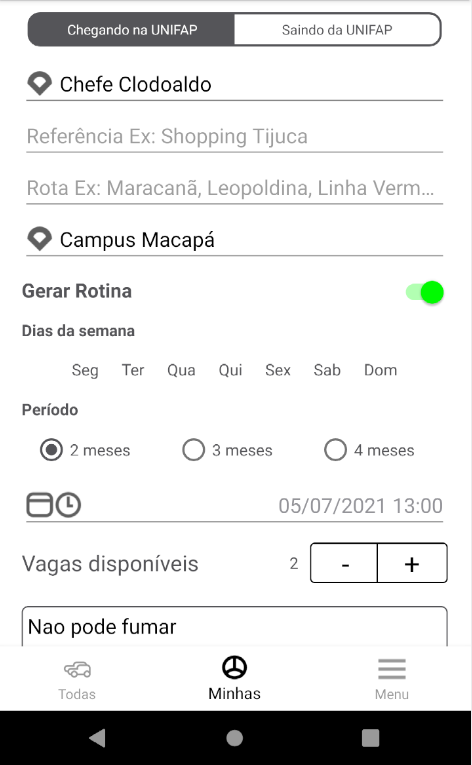
\includegraphics[width=0.29\textwidth]{./04-figuras/caronae/criacao_da_carona_carona_ufrj.png}
	\label{fig:publicar_carona}
	\fonte{Elaborada pelo autor} %acesso: 13/04/2021 
\end{figure}

O aplicativo exige que o usuário nas viagens de ida até a UFRJ tenha como ponto inicial algum bairro de uma das zonas cadastradas no sistema e como destino algum dos pontos/hubs da UFRJ. Nas viagens de volta é o contrário. Com capacidade de oferecer várias viagens durante o ano letivo, os criadores desenvolveram uma funcionalidade que permitisse os motoristas de agendar caronas futuras sem a necessidade de anunciar diariamente as caronas, característica automática que diferencia o Caronaê de outros pontos geradores de viagens (PGV) semelhantes.

Na lista disponibilizada no aplicativo, o usuário pode escolher entre as caronas ofertadas, ver detalhes sobre o trajeto e motorista, e caso lhe agrade, solicitar a carona. Já o motorista que ofereceu a carona pode aceitar ou não e acessar informações do caronista, caso aceite a corrida, um alerta é enviado para o caronista. O aplicativo também fornece aos envolvidos na corrida, um chat, informações adicionais como placa, cor do carro e modelo. A figura \ref{fig:solicitacao_de_carona} mostra a tela de solicitação de carona com a origem de um bairro da cidade e o destino o Campus Macapá.

\begin{figure}[!hbtp]
	\centering
	\caption{Notificação: Solicitação de Carona}
	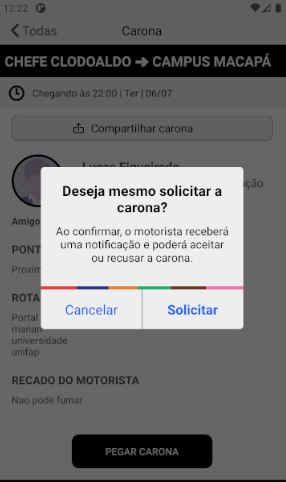
\includegraphics[width=0.29\textwidth]{./04-figuras/caronae/tela_solicitacao_de_carona_2.png}
	\label{fig:solicitacao_de_carona}
	\fonte{Elaborada pelo autor} %acesso: 13/04/2021 
\end{figure}

O "Meu Perfil" é possível ver as informações do usuário, se for o motorista, aparece as informações do veículo, número de caronas ofertadas e recebidas, no "Histórico", o usuário motorista consegue acompanhar quantas caronas foram concluídas ou quantas estão pendentes, e o caronista consegue ver quantas caronas pegou. Além disso, o sistema tem o "Falaê", onde os usuários pode manifestar suas sugestões ou críticas, e antes de tudo, o usuário precisa aceitar os termos de uso que também consta no aplicativo. Podemos ver isso na figura \ref{fig:telas_caronae}. 

\begin{figure}[!hbtp]
	\centering
	\caption{Telas do aplicativo Caronaê: login, busca e detalhe da carona}
	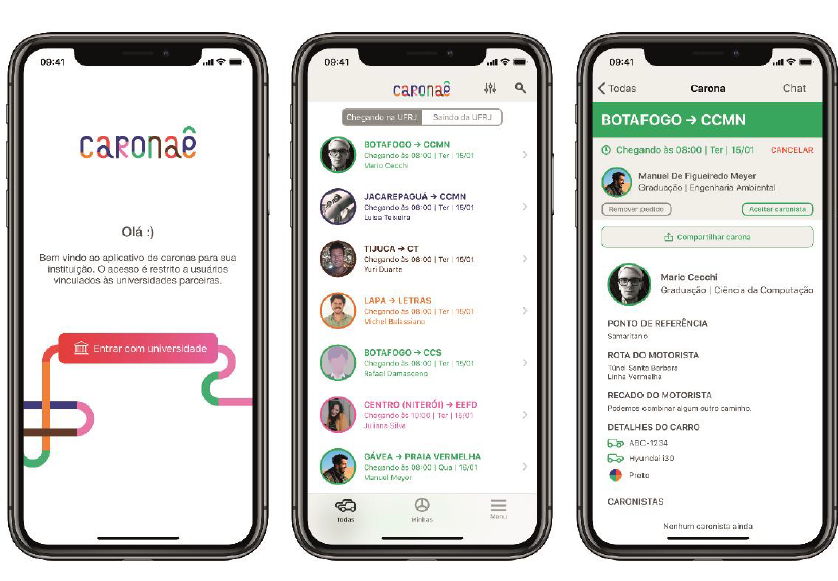
\includegraphics[width=0.5\textwidth]{./04-figuras/caronae-img-artigo.png}
	\label{fig:telas_caronae}
	\fonte{\cite{caronae}}
\end{figure}


Como plataforma digital, o caronaê possui um banco de dados onde registra todas as informações e interações dos serviços. O banco de dados do Caronaê é PostgreSQL, banco de dados objeto-relacionado acessado pela ferramenta administradora PGAdmin4 \footnote{https://www.pgadmin.org/}. O projeto também possuí uma área administrativa contruída com o framework laravel, onde os administradores tem acesso aos dados gerados na aplicação sem precisar realizar a consulta diretamente ao banco, o que exigiria conhecimento da linguagem SQL. \footnote{\textit{StructureStructure Query Language}: é a linguagem de pesquisa declarativa padrão para banco de dados relacional.} 

O sistema inicialmente era hospedado nos servidores da UFRJ, estando exposto a qualquer tipo de instabilidade. Após expandir e ter vários acessos simultâneos, a hospedagem da universidade já não supria a demanda, e os responsáveis pelo projeto começaram a ter problemas de disponibilidade por conta da infraestrutura. Para manter o sistema em funcionamento, a solução foi migrar todo o serviço próprio do Caronaê (backend, sistema administrativo, sistema intermediário de autenticação) para a "nuvem", utilizando a IaaS da empresa Amazon por 3 anos, entre os anos de 2016 e 2019. Após esse período o projeto foi descontinuado \cite{caronae}. 

Para finalizar o resumo das características da solução, o Caronaê, pensando na segurança do usuário, garante o acesso somente à comunidade acadêmica, para garantir isso, o aplicativo se conecta à base de dados da UFRJ através do sistema de gestão, onde busca os dados do aluno no SIGA(nome, curso, foto, se é Servidor, se está na Graduação, Mestrado). O acesso se dá pelo CPF e senha do usuário ativo na UFRJ. Segundo \cite{caronae}, durante o desenvolvimento da pesquisa, essa premissa resultou na criação de um portal específico na Intranet da UFRJ, especifico para os registros do serviço, nele constava todas informações dos usuários, como por exemplo, faixa etária e gênero, essas informações, segundo ela era relevante, a ausência dificultava nas consultas.

Os serviços utilizados para a autenticação dos usuários são \footnote{Disponível em: https://github.com/caronae/caronae-ufrj-authentication. Acesso: 06 Jun. 2021}:

\begin{itemize}
   

 \item \textbf{phpCas:} biblioteca que faz a integração com o CAS (Central Authentication Service) da Intranet UFRJ, que valida que o usuário é vinculado à UFRJ

 \item \textbf{SigaService:} comunica com o SIGA UFRJ, de onde são buscados os dados dos usuários 

 \item \textbf{CaronaeService:} parte do caronae-sdk-php \footnote{Disponivel em: https://github.com/caronae/caronae-sdk-php. Acesso em: 06 Jun. 2021}, é a classe que faz a comunicação com a API do Caronaê e é usada para enviar os dados do usuário para o Caronaê

 \item \textbf{CaronaeSigaAdaptor:} faz a conversão dos dados no formato que vem do SIGA para o formato da API do Caronaê

 \item \textbf{CaronaeUFRJAgent:} faz o fluxo de autenticação e autorização integrando todos os serviços acima
\end{itemize}


\begin{figure}[!hbtp]
	\centering
	\caption{Fluxograma da autenticação do Caronaê}
	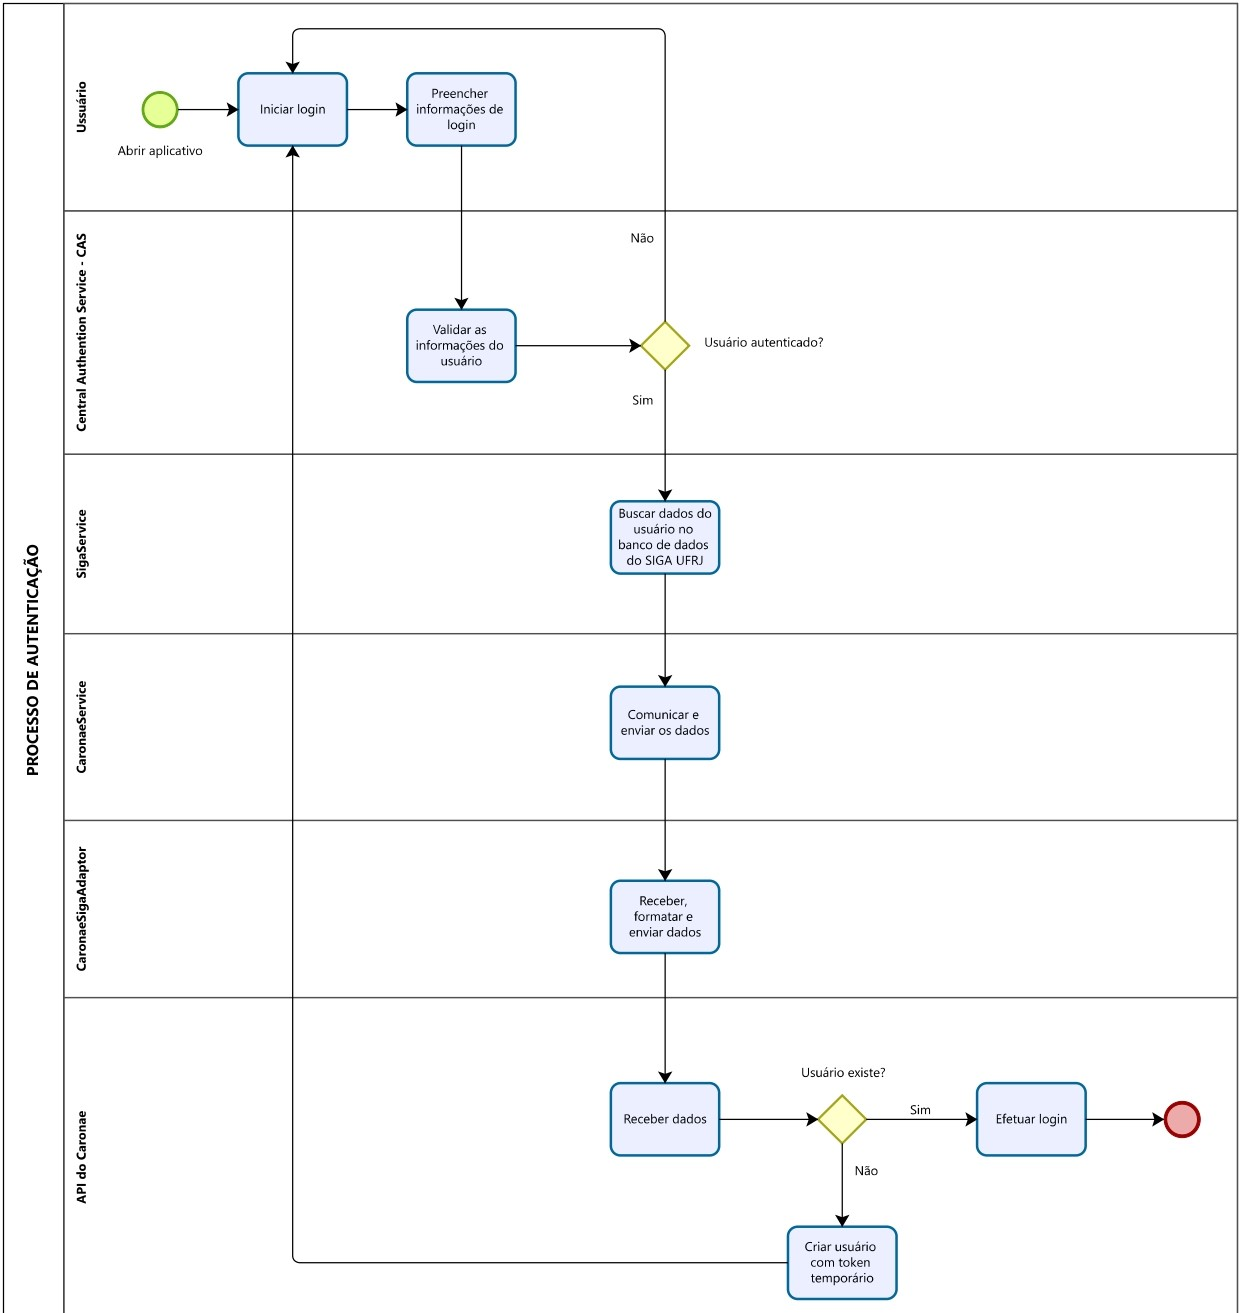
\includegraphics[width=0.6\textwidth]{./04-figuras/caronae/diagrama_bizagi.jpg}
	\label{fig:fluxograma}
	\fonte{Elaborada pelo autor.}
\end{figure}



\begin{comment}
%
	\mnote{Patrícia: falar sobre as características do Caronaê para a UFRJ, as que foram levantadas na análise de requisitos deles e que foram implementadas.}
    % Comentado só para sumir o texto do lado do documento
\end{comment}

\subsection{Características do Caronaê para UNIFAP}

Inicialmente, as mudanças realizadas para o aplicativo se adequar com a realidade dos usuários da UNIFAP foi alterar as zonas e bairros que se encontram no site da prefeitura de Macapá \footnote{https://macapa.ap.gov.br/portal/wp-content/uploads/2020/11/DIVISAO-POR-TERRITORIOS.pdf}, informando a zona e quais bairros pertencem aquela zona. Outras mudanças realizadas foram as alterações de campos que aparecem UFRJ para UNIFAP, na figura \ref{fig:carona_ate_a_unifap} mostra o bairro selecionado na tela do aplicativo.

\begin{figure}[!hbtp]
	\centering
	\caption{Tela de criação de carona: Chegando na Unifap}
	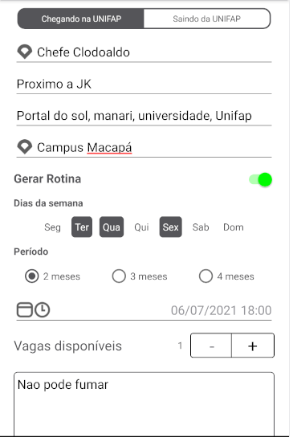
\includegraphics[width=0.17\textwidth]{./04-figuras/caronae/tela_criacao_da_carona_de_chegada_na_unifap.png}
	\label{fig:carona_ate_a_unifap}
	\fonte{Elaborada pelo autor.}
\end{figure}

Pontos de encontro ou Hubs, no qual ajuda os motoristas e caroneiros a se encontrarem também foram adicionados no sistema, levamos em consideração os departamentos da UNIFAP, DCET, DED, DEAD, DFCH, DEMAD, DEPLA, DCBS, Reitoria. Na figura \ref{fig:carona_saindo_da_unifap} podemos ver o cadastro da carona saindo da unifap, onde semelhante a carona chegando a Unifap selecionamos o bairro de saída e chega, uma referência da localização os bairros por onde vai passar com uma diferença, na saída da Unifap, o usuário precisa selecionar o ponto de encontro.

\begin{figure}[!hbtp]
	\centering
	\caption{Tela da criação de carona: Saindo da Unifap}
	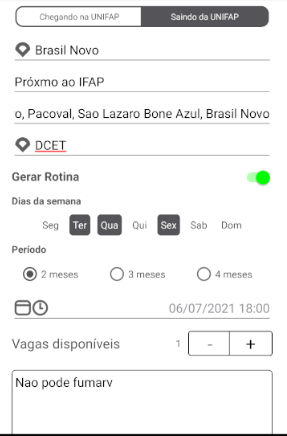
\includegraphics[width=0.25\textwidth]{./04-figuras/caronae/tela_criacao_da_carona_de_saida_da_unifapp.png}
	\label{fig:carona_saindo_da_unifap}
	\fonte{Elaborada pelo autor.}
\end{figure}

Além destes pontos mencionados, o Caronaê para a Universidade também tem como característica o acesso apenas por pessoas ligadas a Unifap, porém, diferente da UFRJ, não temos uma solução que disponibilize os dados dos alunos, professores e técnicos para a solução consumir. Na figura \ref{fig:tela_usuarios_painel_administrativo} mostra o painel administrativo do Caronaê, onde é gerenciado usuários, caronas, zonas e bairros, administradores instituições, onde é possível bloquear usuários caso seja necessário, entre outras funções, na figura podemos ver alguns nomes de usuários e informações que foram geradas em um banco de dados fictício, mas que em produção utiliza de serviços para consumir da base de dados real da universidade.

\begin{figure}[!hbtp]
	\centering
	\caption{Tela da criação de carona: Saindo da Unifap}
	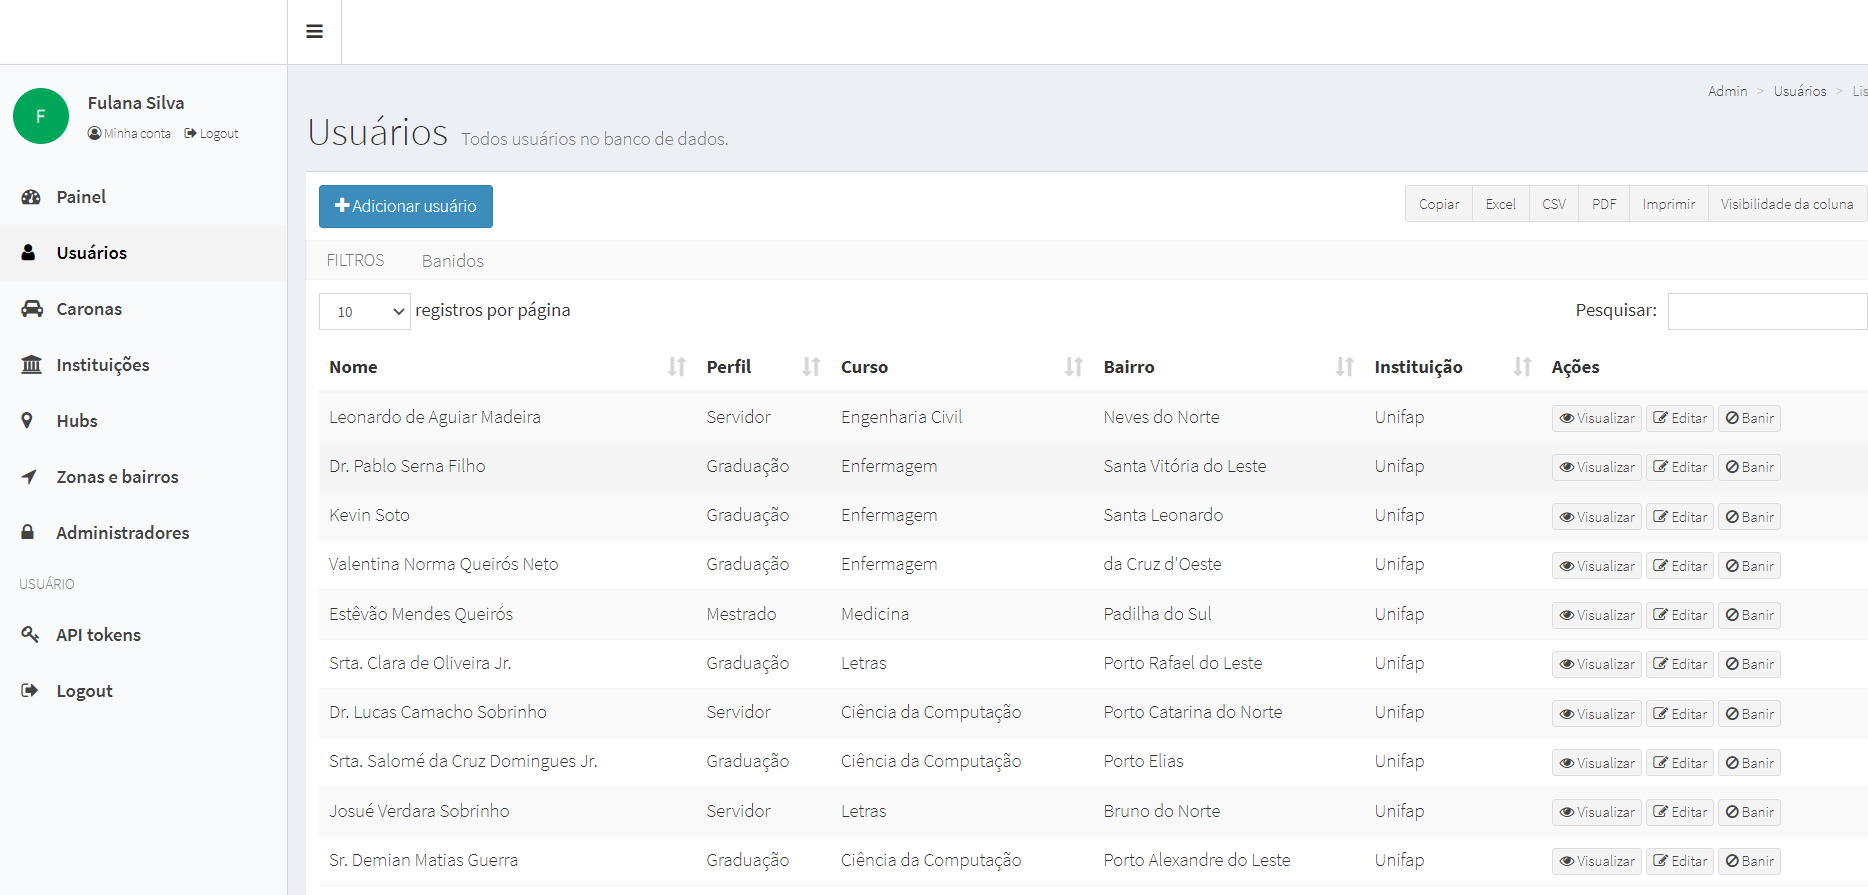
\includegraphics[width=0.9\textwidth]{./04-figuras/caronae/tela_usuarios_do_painel_administrativo.png}
	\label{fig:tela_usuarios_painel_administrativo}
	\fonte{Elaborada pelo autor.}
\end{figure}

No momento, para utilizar o aplicativo estão rodando em um banco de dados PostgreSQL \footnote{https://www.postgresql.org/docs/} local, o serviço de backend e do sistema administrativo pelo servidor local do laravel \footnote{https://laravel.com/} e o emulador do Android Studio\footnote{https://developer.android.com/studio} também localmente.

\begin{comment}
	\mnote{Patrícia: falar sobre que características o Caronaê deveria ter para ser implementado na UNIFAP, que características já existentes permaneceriam, que características já existentes devem ser adaptadas ou modificadas, que características já existentes devem ser retiradas e que características devem ser incluídas considerando o contexto da Unifap e Macapá. Isso seria o seu levantamento de requisitos.}
\end{comment}


\begin{comment}

\subsection{Dificuldades Enfrentadas}

As dificuldades iniciais foi a de tentar executar todos os serviços presentes na aplicação, todos os microserviços de aunteticação e notificação do aplicativo, porém, isso não se deu porque a API que auxiliava o projeto, API está, fornecidade pela universidade não está mais online.

Outros microserviços dependem do funcionamento e do acesso as APIs que UFRJ disponibilizava, entretanto, foi deixado de lado essas tentativas e focado apenas na execução local, com banco de dados local, API apenas do Caronaê com dados de alguns usuários que estão cadastrados nas querys do projeto e o no funcionamento do API e integração dos serviços. O fato de não termos uma API na universidade onde eu possa testar a aplicação também dificulta a proposta, claro que antes algumas coisas precisariam ser avaliadas, como o tratamento dos dados do SIGAA UNIFAP para o formato que a API do Caronaê recebe, caso fosse necessário.

\end{comment}

\begin{comment}
\section{Próximos passos}
Será funcionar o aplicativo junto ao back-end da aplicação seja ele utilizando as imagens do docker ou utilizando outros serviços similares aos utilizados, como o XAMPP que oferecem os serviços Apache como servidor Web, Mysql como banco de dados e PHP.

Ainda incluindo também uma forma ou opção de como consumir as informações do sistema de gestão da Unifap, algo que pode ser visto mais a frente quando os primeiros passos forem realizados, objetivo contudo é apresentar e mostrar que o código fonte pode ser reaproveitado e dado continuidade numa ideia interessante realizada pela equipe Caronaê.
\end{comment}


   	%
% Documento: Cronograma
%

\chapter{Cronograma}\label{chap:Cronograma} 

O desenvolvimento deste trabalho se dará da seguinte forma:

\begin{enumerate}
 	\item \label{um} Elaboração da proposta de TC. %1
	\item \label{dois} Análise do questionário. %2
	\item \label{tres} Estudo sobre cidades inteligentes, campus inteligentes. %3
	\item \label{quatro} Estudo sobre as tecnologias de mobilidade %4 
	\item \label{cinco} Levantamento das tecnologias de mobilidade inteligente existentes. %5
	\item \label{seis}  Análise das Tecnologias de mobilidade inteligente %6
	\item \label{sete} Levantamento de requisitos da solução escolhida %7
	
	\item \label{oito} Estudo das tecnologias necessárias para utilizar o  Caronaê (Laravel, Postgresql, Nginx, Java, Android Studio) 
	\item \label{nove} Teste do Caronaê e dos Serviços do Caronaê. %10
	\item \label{dez} Alterações no código para funcionar em localhost. %11
	\item \label{onze} Alterando dados e informações para adequar o Caronaê à UNIFAP.
	\item \label{doze}  Escrita do Pré-projeto.
	\item \label{treze} Apresentação do Pré-projeto
	\item \label{catorze} Adicionar todos os requisitos do Caronaê.
	\item \label{quinze} Escrita do Trabalho Final.
\end{enumerate}

\begin{landscape}
\definecolor{midgray}{gray}{.5}
\begin{table}[!htbp]
    \centering
		\begin{tabular}{|c|c|c|c|c|c|c|c|c|c|c|c|c|c|c|c|c|c|}
		\hline
		&\multicolumn{5}{c|}{2020}&\multicolumn{12}{c|}{2021}\\
		\hline
		&AGO&SET&OUT&NOV&DEZ&JAN&FEV&MAR&ABR&MAI&JUN&JUL&AGO&SET&OUT&NOV&DEZ\\
		\hline
		\ref{um}&\cellcolor{midgray}&\cellcolor{midgray}&&&&&&&&&&&&&&&\\
		\hline
		\ref{dois}&&\cellcolor{midgray}&&&&&&&&&&&&&&&\\
		\hline	
		\ref{tres}&&\cellcolor{midgray}&&&&&&&&&&&&&&&\\
		\hline			
		\ref{quatro}&&\cellcolor{midgray}&\cellcolor{midgray}&&&&&&&&&&&&&&\\
		\hline	
		\ref{cinco}&&&\cellcolor{midgray}&\cellcolor{midgray}&&&&&&&&&&&&&\\
		\hline
		\ref{seis}&&&&\cellcolor{midgray}&\cellcolor{midgray}&&&&&&&&&&&&\\
		\hline	
		\ref{sete}&&&&&\cellcolor{midgray}&\cellcolor{midgray}&&&&&&&&&&&\\
		\hline	
		\ref{oito}&&&&&\cellcolor{midgray}&\cellcolor{midgray}&\cellcolor{midgray}&&&&&&&&&&\\
		\hline	
		\ref{nove}&&&&&&&\cellcolor{midgray}&\cellcolor{midgray}&&&&&&&&&\\
		\hline	
		\ref{dez}&&&&&&&&&\cellcolor{midgray}&&&&&&&&\\
		\hline	
		\ref{onze}&&&&&&&&&\cellcolor{midgray}&\cellcolor{midgray}&&&&&&&\\
		\hline	
		\ref{doze}&&&&&&&&&&\cellcolor{midgray}&\cellcolor{midgray}&\cellcolor{midgray}&&&&&\\
		\hline	
		\ref{treze}&&&&&&&&&&&&\cellcolor{midgray}&&&&&\\
		\hline
		
		\ref{catorze}&&&&&&&&&&&&\cellcolor{midgray}&\cellcolor{midgray}&\cellcolor{midgray}&\cellcolor{midgray}&\cellcolor{midgray}&\cellcolor{midgray}\\
		\hline	
		\ref{quinze}&&&&&&&&&&&&\cellcolor{midgray}&\cellcolor{midgray}&\cellcolor{midgray}&\cellcolor{midgray}&\cellcolor{midgray}&\cellcolor{midgray}\\
		\hline	
		\end{tabular}
\end{table}
\end{landscape}
   	%%
% Documento: Suprimentos
%

\chapter{Suprimentos e Equipamentos}\label{chap:suprimentos} 

Para realização desta pesquisa, foi elaborado um questionário utilizando a  ferramenta gratuita do Google Formulário e disponibilizado para os alunos da comunidade acadêmica interessados durante o período de Abril de 2019 a Dezembro de 2019, com a intenção de entender o perfil dos acadêmicos e profissionais  da universidade, buscando entender se seria  viável e interessante para estes o uso de um aplicativo com a intenção de facilitar a acessibilidade até o campus Macapá da Universidade Federal do Amapá.

Foi também utilizado meios digitais para o compartilhamento do formulário, mensagens em grupos de cursos com o link de direcionamento ao formulário, impressão de informativos explicando o motivo da pesquisa com o endereço do formulário em QR Code , estas impressões foram espalhadas pela universidade. 

   	%%
% Documento: Custos
%

\chapter{Custos}\label{chap:custos}
   	%%
% Documento: Anexos
%

\chapter{Anexos}\label{chap:anexos}
   	%%
% Documento: Apêndices
%

\chapter{Apêndices}\label{chap:apendices}
   	 %
% Documento: Referências Bibliográficas
%
\bibliography{./refbase}    % Geração automática das referências por meio do arquivo 'refbase.bib'

    

\end{document}
